% ============================================================
% Savoury - Hostel Mess Management System
% UCS503 Software Engineering Project Report (End-Semester Evaluation)
%
% Compile with pdfLaTeX (Overleaf default) or XeLaTeX/Tectonic.
%
% Screenshots: every image in this report is a placeholder box that
% describes what the screenshot must show. Create a folder named
% "screenshots" next to this file and save each image under the file
% name printed in its placeholder (e.g. screenshots/web-checkin.png).
% The box is replaced by the image automatically on the next compile.
% ============================================================
\documentclass[11pt,a4paper]{article}

\usepackage{iftex}
\ifPDFTeX
  \usepackage[T1]{fontenc}
  \usepackage[utf8]{inputenc}
  \usepackage{mathptmx}
\else
  \usepackage{mathptmx}
  \usepackage{fontspec}
  \setmainfont{texgyretermes}[Extension=.otf,UprightFont=*-regular,BoldFont=*-bold,ItalicFont=*-italic,BoldItalicFont=*-bolditalic]
\fi
\usepackage[margin=2.5cm,headheight=14pt]{geometry}
\usepackage{amsmath,amssymb}
\usepackage{graphicx}
\usepackage[table]{xcolor}
\usepackage{array,booktabs,tabularx,longtable,multirow}
\usepackage{ragged2e}
\usepackage{enumitem}
\usepackage{fancyhdr}
\usepackage{float}
\usepackage[labelfont=bf,font=small,labelsep=colon]{caption}
\usepackage{tikz}
\usetikzlibrary{positioning,arrows.meta,shapes.geometric,shapes.multipart,shapes.misc,fit,calc,backgrounds,shadows}
\usepackage[hidelinks]{hyperref}

\setlength{\parindent}{0pt}
\setlength{\emergencystretch}{3em}
\setlength{\parskip}{0.55em}
\renewcommand{\arraystretch}{1.25}
\setlist{itemsep=0.2em,topsep=0.3em}
\newcolumntype{L}[1]{>{\RaggedRight\arraybackslash}p{#1}}
\newcolumntype{Y}{>{\RaggedRight\arraybackslash}X}

% ---------- header / footer ----------
\pagestyle{fancy}
\fancyhf{}
\lhead{\small UCS503 -- Software Engineering Lab}
\rhead{\small Savoury}
\cfoot{\thepage}
\renewcommand{\headrulewidth}{0.4pt}

% ---------- screenshot placeholder ----------
% \shot{file}{box height}{description}
\definecolor{phborder}{RGB}{150,150,150}
\definecolor{phfill}{RGB}{246,246,246}
\definecolor{phtitle}{RGB}{176,58,46}
\newcommand{\shot}[3]{%
  \IfFileExists{#1}{%
    \includegraphics[width=\linewidth,height=#2,keepaspectratio]{#1}%
  }{%
    \fcolorbox{phborder}{phfill}{%
      \parbox[c][#2][c]{0.94\linewidth}{\centering
        {\small\bfseries\color{phtitle}[ SCREENSHOT PLACEHOLDER ]}\\[0.35em]
        {\footnotesize\ttfamily #1}\\[0.7em]
        \parbox{0.88\linewidth}{\RaggedRight\small #3}}}%
  }}

% ---------- TikZ styles ----------
\tikzset{
  >={Stealth[length=2.4mm]},
  every picture/.style={line width=0.6pt},
  every node/.append style={execute at begin node={\hyphenpenalty=10000\exhyphenpenalty=10000}},
  uc/.style={ellipse, draw, fill=blue!7, minimum width=3.7cm, minimum height=0.95cm,
             align=center, font=\small, inner sep=1pt},
  act/.style={rectangle, rounded corners=5pt, draw, fill=blue!8, align=center,
              font=\small, text width=4.0cm, minimum height=0.8cm},
  actr/.style={act, fill=red!10},
  actg/.style={act, fill=green!12},
  dec/.style={diamond, draw, fill=yellow!25, aspect=2.3, align=center,
              font=\footnotesize, inner sep=0pt, text width=1.9cm},
  startnode/.style={circle, fill=black, minimum size=0.42cm, inner sep=0pt},
  endnode/.style={circle, draw, double, double distance=1.3pt, fill=black,
                  minimum size=0.36cm, inner sep=0pt},
  proc/.style={rectangle, rounded corners=7pt, draw, fill=green!10, align=center,
               font=\small, text width=3.3cm, minimum height=1.1cm},
  procd/.style={proc, dashed, fill=gray!8},
  ent/.style={rectangle, draw, fill=gray!12, align=center, font=\small,
              minimum height=0.9cm, minimum width=2.4cm},
  store/.style={rectangle, font=\small, minimum height=0.7cm, inner xsep=5pt,
                minimum width=3.4cm, align=left,
                append after command={
                  (\tikzlastnode.north east) edge[-] (\tikzlastnode.north west)
                  (\tikzlastnode.north west) edge[-] (\tikzlastnode.south west)
                  (\tikzlastnode.south west) edge[-] (\tikzlastnode.south east)}},
  flow/.style={->, font=\scriptsize},
  lbl/.style={font=\scriptsize, fill=white, inner sep=1.5pt, align=center},
  cls/.style={rectangle split, rectangle split parts=3, draw, fill=white,
              font=\scriptsize, align=left, text width=#1,
              rectangle split part fill={blue!10,white,white}},
  cls/.default=4.1cm,
  st/.style={rectangle, rounded corners=8pt, draw, fill=yellow!20, align=center,
             font=\small, minimum width=3cm, minimum height=0.9cm},
  str/.style={st, fill=red!10},
  stg/.style={st, fill=green!12},
  comp/.style={rectangle, draw, fill=blue!8, align=center, font=\small,
               text width=2.9cm, minimum height=1cm},
  lifeline/.style={rectangle, draw, fill=blue!8, font=\footnotesize,
                   minimum height=0.65cm, inner xsep=4pt},
  card/.style={rectangle, rounded corners=4pt, draw, fill=yellow!12,
               text width=7.1cm, inner sep=6pt, align=left, font=\small},
  note/.style={rectangle, draw, fill=gray!8, font=\footnotesize, align=left, inner sep=4pt},
}

% stick-figure actor: \actor{coordinate name}{(x,y)}{label}
\newcommand{\actor}[3]{%
  \begin{scope}[shift={#2}]
    \draw (0,0.62) circle (0.19);
    \draw (0,0.43) -- (0,-0.08);
    \draw (-0.32,0.22) -- (0.32,0.22);
    \draw (0,-0.08) -- (-0.24,-0.5);
    \draw (0,-0.08) -- (0.24,-0.5);
    \node[below, font=\small\bfseries, align=center] at (0,-0.5) {#3};
    \coordinate (#1) at (0,0.15);
  \end{scope}}

\hypersetup{pdftitle={Savoury - UCS503 Final Project Report},pdfauthor={Siddharth Singla, Vineet Tripathi, Shivansh Sahu}}

\begin{document}

% ============================================================
% TITLE PAGE
% ============================================================
\begin{titlepage}
\thispagestyle{empty}
\centering
{\large UCS503 -- Software Engineering Lab\par}
\vspace{3.2cm}
{\fontsize{30}{36}\selectfont\bfseries Savoury\par}
\vspace{0.8cm}
{\Large Hostel Mess Management System with\\[0.3em]
Cutoff-Driven Booking and Wallet-Based Billing\par}
\vspace{1.8cm}
{\large UCS 503 Software Engineering Project Report\par}
\vspace{0.6cm}
{\large\bfseries END-Semester Evaluation\par}
\vspace{2.6cm}

\begin{minipage}[t]{0.55\textwidth}
\raggedright
\textbf{Submitted by:}\\[0.5em]
(1024170252) Siddharth Singla\\
(1024170253) Vineet Tripathi\\
(1024170249) Shivansh Sahu\\[1em]
BE Third Year, COE
\end{minipage}\hfill
\begin{minipage}[t]{0.38\textwidth}
\raggedleft
\textbf{Submitted to:}\\[0.5em]
% TODO: replace with the name of your lab instructor
[Instructor Name]
\end{minipage}

\vfill
{\large Computer Science and Engineering Department\par}
\vspace{0.4em}
{\large TIET, Patiala\par}
\vspace{0.4em}
{\large November 2026\par}
\end{titlepage}

% ============================================================
% FRONT MATTER
% ============================================================
\pagenumbering{roman}
\renewcommand{\contentsname}{\centering TABLE OF CONTENTS}
\tableofcontents
\clearpage
\listoffigures
\listoftables
\clearpage
\pagenumbering{arabic}

% ============================================================
\section{Project Selection Phase}
% ============================================================
\subsection{Software Bid}

\textbf{Project title.} Savoury: a hostel mess management system with
cutoff-driven meal booking, counter check-in and wallet-based billing.

\textbf{Problem statement.} Hostel messes at TIET charge every resident a flat
fee and plan food from guesswork. A student who goes home for the weekend, eats
out or skips breakfast still pays for every meal, and the kitchen still cooks
for them. Headcounts are estimated from habit, so food is either wasted or runs
out. Attendance, refunds and balances live in paper registers, WhatsApp groups
and spreadsheets, which makes reconciliation slow and disputes common. Wardens
have no live picture of how many students will eat a given meal, and students
have no transparent record of what they were charged and why.

\textbf{Proposed solution.} Our team bids to build Savoury, a client--server
platform made of one shared REST backend, a mobile app for students and a web
console for hostel staff. Every student is assumed to eat every meal
(\emph{implicit opt-in}) and opts out of the meals they will miss before a
configurable cutoff, set separately for breakfast, lunch and dinner in Indian
Standard Time. At the cutoff the booking is locked, so the kitchen gets a final
expected headcount. At the counter, mess staff search the student by roll number
and tap \emph{Serve}; the server records the attendance and deducts the
per-meal rate (Rs.\ 75.00 in the pilot configuration) from the student's prepaid
wallet in a single database transaction. Wardens top up wallets, approve
end-of-semester cashouts, publish menus and notices and watch expected-versus-served
counts on a live dashboard.

\textbf{Scope of the bid.} The delivered system covers a one-time Super Admin
setup, student self-registration with a college e-mail and e-mail verification,
staff login, hostel and fee-plan management, role management for seven roles,
per-meal opt-in and opt-out, date-range absences, the hourly booking-lock job,
counter check-in with duplicate and opt-out protection, walk-in overrides,
the live headcount dashboard, the wallet ledger with top-ups, deductions and
cashouts, hostel-scoped menus and notices. Guest meals, meal feedback and the
audit log are modelled in the database but are deferred to a later release.
Online payment collection is outside the scope; top-ups are recorded by the
warden after payment is received through the institute's existing channel.

\textbf{Team and responsibilities.} The work was divided by subsystem so that
each member owned a complete vertical slice. Table~\ref{tab:team} lists the
allocation.

% TODO: confirm the module ownership below with the team before submission.
\begin{table}[H]
\centering
\caption{Team members and module ownership}
\label{tab:team}
\begin{tabular}{@{}L{2.2cm}L{3.2cm}L{9.4cm}@{}}
\toprule
\textbf{Roll No.} & \textbf{Name} & \textbf{Primary responsibility}\\
\midrule
1024170252 & Siddharth Singla & Backend API (Express, TypeScript, Prisma schema and
migrations), IST cutoff computation and booking-lock job, attendance and wallet
transactions, security hardening, deployment on Render and Supabase, CI pipeline.\\
1024170253 & Vineet Tripathi & Web console (React and Vite): login and setup,
counter check-in page with its offline sync queue, headcount dashboard, users,
wallet, menu, hostels, fee-plan and notices pages.\\
1024170249 & Shivansh Sahu & Mobile app (Expo and React Native): registration
and login, home screen meal cards, opt-out calendar, wallet and cashout,
notices and profile; design of the manual test cases.\\
\bottomrule
\end{tabular}
\end{table}

\textbf{Technical feasibility.} Every building block is mature and free to use.
Express with TypeScript gives a typed REST service, Prisma provides schema
migrations, typed queries and interactive transactions over PostgreSQL, and Zod
validates every request body. React with Vite and TanStack Query is a fast
basis for the staff console, and Expo lets one TypeScript code base produce the
Android and iOS student app. The only hard problems are business rules
(cutoffs in IST, implicit opt-in, transactional billing, hostel scoping), not
algorithms, so the risk sits in correctness rather than in research.

\textbf{Economic feasibility.} All libraries are open source. The backend runs
on the free plan of Render, the web console on Vercel, the database on the free
tier of Supabase and verification e-mail on the free tier of Brevo. Verification
is optional: with no Brevo key configured, accounts are usable immediately. The
project can therefore be developed, demonstrated and piloted at zero recurring
cost; the investment is the development time of three students across the
semester.

\textbf{Operational feasibility.} Students already carry Android or iOS phones
and the mess counter already has a computer or tablet with a browser. The
student flow has one decision per meal (eat or skip), and the counter flow has
one action per student (search and serve). Times are always shown in IST, so
nobody needs to convert time zones.

\textbf{Development plan.} Table~\ref{tab:phases} summarises the phases the
team followed during the semester.

\begin{table}[H]
\centering
\caption{Planned phases and deliverables}
\label{tab:phases}
\begin{tabular}{@{}L{3.6cm}L{11.2cm}@{}}
\toprule
\textbf{Phase} & \textbf{Deliverable}\\
\midrule
Selection and analysis & Product requirements document, project proposal,
SRS with numbered functional requirements, user stories.\\
Design & Data model (Prisma schema), role matrix, REST API areas, UML and DFD
diagrams.\\
Implementation 1 & Authentication, hostels and users, meal types, menus,
bookings and the IST cutoff rule.\\
Implementation 2 & Counter check-in, attendance with wallet deduction, headcount
dashboard, wallet top-ups and cashouts.\\
Implementation 3 & Co-Warden and Caretaker roles, date-range opt-outs, notices,
e-mail verification, security hardening, insufficient-balance guard.\\
Testing and review & Automated Jest suites, CI on every pull request,
manual test cases in the Doc:T\_01 template, peer review and final report.\\
\bottomrule
\end{tabular}
\end{table}

\textbf{Risks and mitigation.} The first risk is \emph{time-zone errors}: the
server runs in UTC while every meal time is an IST wall-clock time, and an early
version fired every cutoff 5.5 hours late. We mitigate it by converting each
configured IST time to its exact UTC instant in one function and testing that
function against fixed UTC instants. The second risk is \emph{double charging}
when two counters serve the same student at once. A unique constraint on the
booking of an attendance record and a conditional balance decrement inside one
transaction make the second attempt fail without side effects. The third risk is
\emph{cross-hostel access}: every staff action is checked against the hostel of
the acting user, which is loaded from the database on each request instead of
being trusted from the token. The fourth risk is an \emph{unreliable network at
the counter}; the check-in page queues serves locally and replays them when the
connection returns, and the server's duplicate check makes replays safe.

\subsection{Project Overview}

Savoury is organised as three clients that share one backend. The
\textbf{backend API} is a layered Express application:
routes $\rightarrow$ middleware (\texttt{authenticate}, \texttt{authorizeRoles})
$\rightarrow$ controllers (Zod validation and HTTP) $\rightarrow$ services
(business rules) $\rightarrow$ Prisma $\rightarrow$ PostgreSQL. It applies
\texttt{helmet}, a CORS allow-list, a 1 MB body limit, a global rate limiter and
a stricter limiter on \texttt{/auth}, and mounts ten routers:
\texttt{/auth}, \texttt{/menu}, \texttt{/bookings}, \texttt{/attendance},
\texttt{/hostels}, \texttt{/users}, \texttt{/wallet}, \texttt{/opt-outs},
\texttt{/config} and \texttt{/notices}, plus \texttt{/health}. A cron job runs
at the start of every hour and locks open bookings whose cutoff has passed.

The \textbf{student mobile app} opens on a home screen that shows today's menu
as one card per meal. Each card states whether the student is opted in and
whether the meal is still open; one tap opts out or back in. An opt-out
calendar schedules whole-day absences over a date range, the wallet screen
shows the balance, the transaction history and the cashout button, and the
notices screen lists announcements for the student's hostel.

The \textbf{staff web console} adapts its sidebar to the signed-in role. Mess
Staff see only Check-In, where they pick the meal, search by name or roll number
and tap \emph{Serve}. Hostel admins (Warden, Co-Warden and Caretaker) also see
the Headcount dashboard, Menu, Users, Wallet and Notices; the Super Admin
additionally manages hostels and fee plans. The dashboard shows, for each meal of
the selected day, the expected count (students minus opt-outs), the served count,
the served percentage and a status badge: Upcoming, Final (cutoff passed),
Active (serving now) or Over (serving window ended).

Money moves in exactly one place. When a student is served, the attendance
service creates the attendance row, checks that the wallet balance covers the
meal rate, decrements the balance and writes a \texttt{MEAL\_DEDUCTION} ledger
entry, all inside one Prisma transaction. If any step fails, none of them is
kept. Throughout the design the system follows two principles: a student who is
not served is never charged, and no user can see or change another hostel's
data.

% ============================================================
\clearpage
\section{Analysis Phase}
% ============================================================
\subsection{Use Cases}
\subsubsection{Use-Case Diagrams}

Figure~\ref{fig:usecase} shows the functional scope of Savoury from the point
of view of its users. The \emph{Student} is the primary actor of the mobile app.
The \emph{Mess Staff}, \emph{Hostel Admin} (Warden, Co-Warden or Caretaker) and
\emph{Super Admin} are the primary actors of the web console. The
\emph{Brevo e-mail service} is a secondary actor that delivers verification
links. A \emph{Mess Committee} member is a student with extra privileges, so it
inherits every student use case and additionally serves at the counter, views
the headcount and manages menus and notices. Three behaviours are always part of
a larger use case and are therefore modelled as \guillemotleft include\guillemotright{}
relationships: registering always sends a verification e-mail (when e-mail is
configured), opting out always enforces the meal cutoff, and serving a student
always deducts the meal rate from the wallet. A walk-in override is an optional
variant of serving and is modelled as an \guillemotleft extend\guillemotright{}
relationship.

\begin{figure}[H]
\centering
\resizebox{\textwidth}{!}{%
\begin{tikzpicture}
  % system boundary
  \draw[rounded corners=4pt, fill=gray!4] (-2.35,1.35) rectangle (11.75,-10.55);
  \node[font=\bfseries, anchor=north west] at (-2.25,1.3) {Savoury};
  % left column: student use cases
  \node[uc] (L1) at (0,0)    {Register Account};
  \node[uc] (L2) at (0,-1.6) {Log In};
  \node[uc] (L3) at (0,-3.2) {Opt In / Out\\of a Meal};
  \node[uc] (L4) at (0,-4.8) {Schedule Absence\\over a Date Range};
  \node[uc] (L5) at (0,-6.4) {View Menu\\and Notices};
  \node[uc] (L6) at (0,-8.0) {View Wallet and\\Request Cashout};
  % middle column: included use cases
  \node[uc, fill=green!8] (M1) at (4.7,0.15)  {Send Verification\\E-mail};
  \node[uc, fill=green!8] (M3) at (4.7,-2.25) {Deduct Meal Rate\\from Wallet};
  \node[uc, fill=green!8] (M2) at (4.7,-4.0)  {Enforce Meal\\Cutoff};
  % right column: staff use cases
  \node[uc] (R1) at (9.4,0)    {Serve Student\\at Counter};
  \node[uc] (R2) at (9.4,-1.6) {Record Walk-in\\Override};
  \node[uc] (R3) at (9.4,-3.2) {View Live\\Headcount};
  \node[uc] (R4) at (9.4,-4.8) {Manage Menu\\and Notices};
  \node[uc] (R5) at (9.4,-6.4) {Top Up Wallet /\\Approve Cashout};
  \node[uc] (R6) at (9.4,-8.0) {Manage Users\\and Roles};
  \node[uc] (R7) at (9.4,-9.6) {Manage Hostels\\and Fee Plans};
  % include / extend
  \draw[dashed,->] (L1) -- node[lbl, above, sloped]{\guillemotleft include\guillemotright} (M1);
  \draw[dashed,->] (L3) -- node[lbl, above, sloped]{\guillemotleft include\guillemotright} (M2);
  \draw[dashed,->] (L4) -- node[lbl, below, sloped]{\guillemotleft include\guillemotright} (M2);
  \draw[dashed,->] (R1) -- node[lbl, above, sloped]{\guillemotleft include\guillemotright} (M3);
  \draw[dashed,->] (R2) -- node[lbl, below, sloped]{\guillemotleft include\guillemotright} (M3);
  \draw[dashed,->] (R2) -- node[lbl, right]{\guillemotleft extend\guillemotright} (R1);
  % actors
  \actor{stu}{(-4.4,-4.0)}{Student}
  \actor{com}{(-4.4,-8.9)}{Mess\\Committee}
  \actor{brv}{(4.7,2.7)}{}
  \node[font=\small\bfseries, right] at (5.0,2.85) {Brevo E-mail Service};
  \actor{msf}{(13.7,0.0)}{Mess Staff}
  \actor{adm}{(13.7,-4.0)}{Hostel Admin}
  \actor{sad}{(13.7,-8.8)}{Super Admin}
  % generalisation: committee -> student
  \draw[-{Triangle[open,length=3mm,width=3mm]}] (-4.4,-8.1) -- (-4.4,-5.35);
  % associations
  \foreach \u in {L1,L2,L3,L4,L5,L6} \draw (stu) -- (\u.west);
  \draw (brv) -- (M1.north);
  \draw (msf) -- (R1.east);
  \foreach \u in {R1,R2,R3,R4,R5,R6} \draw (adm) -- (\u.east);
  \foreach \u in {R6,R7} \draw (sad) -- (\u.east);
\end{tikzpicture}}
\caption{Use-case diagram of Savoury. A Mess Committee member inherits the Student
use cases and is also associated with Serve Student at Counter, View Live
Headcount and Manage Menu and Notices (lines omitted for readability). Every staff
actor also authenticates through Log In on the web console.}
\label{fig:usecase}
\end{figure}

\subsubsection{Use Case Templates}

The following templates describe the most significant use cases in the
structured format used in the course. Each template lists the actors, the
conditions that must hold before and after the use case, the normal sequence of
events and the alternative paths.

\begin{table}[H]
\centering
\caption{Use case template: Register Student Account}
\label{tab:uc1}
\begin{tabular}{@{}L{3.1cm}L{11.7cm}@{}}
\toprule
\textbf{Use case ID} & UC-01\\
\textbf{Use case name} & Register Student Account\\
\textbf{Actors} & Student (primary), Brevo e-mail service (secondary)\\
\textbf{Description} & A student creates an account on the mobile app with a
college e-mail address and is attached to a hostel.\\
\textbf{Pre-conditions} & The app is open on the Sign In screen and at least one
hostel exists.\\
\textbf{Main flow} & (1) The student opens the registration screen. (2) The
student enters name, \texttt{@thapar.edu} e-mail, password, roll number, room
number and 10-digit phone, and selects a hostel. (3) The app sends the form to
\texttt{POST /auth/register}. (4) The backend validates the fields with Zod,
hashes the password with bcrypt and creates a user whose role is always
\texttt{STUDENT}. (5) If e-mail is configured, the backend stores the SHA-256
hash of a random token and asks Brevo to e-mail the verification link.
(6) The student is signed in and sees the home screen.\\
\textbf{Alternate flows} & A non-college e-mail, a password shorter than 6
characters or a phone number that is not 10 digits is refused with a
``Registration Failed'' message. An e-mail already in use returns HTTP 409. If
Brevo rejects the request, the account is kept and the student is told that the
e-mail could not be sent; logging in again re-sends it, or a hostel admin can
verify the account manually.\\
\textbf{Post-conditions} & A Student account exists in the chosen hostel.\\
\textbf{Frequency} & Once per student.\\
\bottomrule
\end{tabular}
\end{table}

\begin{table}[H]
\centering
\caption{Use case template: Opt Out of a Meal}
\label{tab:uc2}
\begin{tabular}{@{}L{3.1cm}L{11.7cm}@{}}
\toprule
\textbf{Use case ID} & UC-02\\
\textbf{Use case name} & Opt Out of a Meal\\
\textbf{Actors} & Student\\
\textbf{Description} & The student tells the mess that they will not eat one
meal on a given day, before that meal's cutoff.\\
\textbf{Pre-conditions} & The student is signed in and the meal's cutoff has not
passed.\\
\textbf{Main flow} & (1) The home screen shows the meal card with ``You're opted
in''. (2) The student taps the toggle. (3) The app calls
\texttt{PUT /bookings/toggle} with status \texttt{OPTED\_OUT}. (4) The backend
computes the cutoff instant from the meal's IST cutoff time and compares it with
the current time. (5) The backend upserts the single booking for
(student, meal, date). (6) The card shows ``Opted out''.\\
\textbf{Alternate flows} & After the cutoff, or if the booking is already
locked, the backend answers HTTP 400 ``Cutoff time has passed for this meal'' and
the card shows ``Closed''. Tapping again before the cutoff opts the student back
in.\\
\textbf{Post-conditions} & Exactly one booking exists for the student, meal and
date, and the headcount for that meal drops by one.\\
\textbf{Frequency} & Several times a week per student.\\
\bottomrule
\end{tabular}
\end{table}

\begin{table}[H]
\centering
\caption{Use case template: Schedule an Absence over a Date Range}
\label{tab:uc3}
\begin{tabular}{@{}L{3.1cm}L{11.7cm}@{}}
\toprule
\textbf{Use case ID} & UC-03\\
\textbf{Use case name} & Schedule an Absence over a Date Range\\
\textbf{Actors} & Student\\
\textbf{Description} & The student opts out of every meal on a range of days,
for example when going home.\\
\textbf{Pre-conditions} & The student is signed in.\\
\textbf{Main flow} & (1) The student opens the Opt-Out Calendar. (2) The student
selects a start day and an end day. (3) The student taps ``Opt Out ($n$d)'' and
confirms. (4) The backend creates one day-level absence per date and sets every
meal that is still before its cutoff to \texttt{OPTED\_OUT}. (5) The app shows
``Opt-Out Confirmed'' with the number of meals and days.\\
\textbf{Alternate flows} & Meals already past their cutoff are skipped and the
response reports how many were kept as they were. If every selected meal is
closed, the request is refused. ``Re-Opt In'' on a scheduled day removes that
absence and reopens only the meals still before their cutoff.\\
\textbf{Post-conditions} & The absences are listed under ``Your Scheduled
Absences'' and the headcount of the affected meals is reduced.\\
\textbf{Frequency} & A few times per semester.\\
\bottomrule
\end{tabular}
\end{table}

\begin{table}[H]
\centering
\caption{Use case template: Serve Student at Counter}
\label{tab:uc4}
\begin{tabular}{@{}L{3.1cm}L{11.7cm}@{}}
\toprule
\textbf{Use case ID} & UC-04\\
\textbf{Use case name} & Serve Student at Counter\\
\textbf{Actors} & Mess Staff (primary); Mess Committee and Hostel Admin may
also serve\\
\textbf{Description} & Staff record that a student took a meal, and the meal is
billed to the student's wallet.\\
\textbf{Pre-conditions} & The staff member is signed in to the web console, the
meal's check-in window is open (60 minutes before serving start to 60 minutes
after serving end, today only) and the student belongs to the staff member's
hostel.\\
\textbf{Main flow} & (1) Staff open Check-In and select the meal. (2) The page
loads the roster: every student of the hostel with booking status and served
flag. (3) Staff type a name or roll number and tap ``Tap to Serve''. (4) The
backend checks the role, the hostel and the time window. (5) In one transaction
it creates a \texttt{SERVED} attendance, decrements the wallet by the per-meal
rate only if the balance covers it, and writes a \texttt{MEAL\_DEDUCTION}
entry. (6) The student moves to the recent check-ins list.\\
\textbf{Alternate flows} & An opted-out student is refused (HTTP 400). A student
of another hostel is refused (HTTP 403). A student without a wallet is refused
(HTTP 422) and an insufficient balance is refused (HTTP 402); in both cases the
attendance row is rolled back. A second serve of the same booking charges
nothing and returns the result \texttt{DUPLICATE}. Without a network the page
queues the serve and replays it later.\\
\textbf{Post-conditions} & One attendance record and one deduction exist for the
booking.\\
\textbf{Frequency} & Hundreds of times per meal.\\
\bottomrule
\end{tabular}
\end{table}

\begin{table}[H]
\centering
\caption{Use case template: Top Up Wallet}
\label{tab:uc5}
\begin{tabular}{@{}L{3.1cm}L{11.7cm}@{}}
\toprule
\textbf{Use case ID} & UC-05\\
\textbf{Use case name} & Top Up Wallet\\
\textbf{Actors} & Hostel Admin\\
\textbf{Description} & A hostel admin credits money received from a student to
the student's wallet for the semester.\\
\textbf{Pre-conditions} & The admin is signed in and the student is in the
admin's hostel.\\
\textbf{Main flow} & (1) The admin opens the Wallet page. (2) The admin searches
the student, enters a positive amount and an optional note. (3) The admin
clicks ``Process Top-Up''. (4) The backend checks the role and hostel, creates
the wallet for the semester if it does not exist, increments the balance and
writes a \texttt{TOPUP} transaction. (5) The page confirms and clears the form.\\
\textbf{Alternate flows} & Students of other hostels do not appear in the search.
The button stays disabled for an amount of zero. A target that is not a student
is refused with HTTP 400.\\
\textbf{Post-conditions} & The student sees the new balance and a ``Top Up''
entry on the mobile app.\\
\textbf{Frequency} & At the start of the semester and whenever a balance runs
low.\\
\bottomrule
\end{tabular}
\end{table}

\begin{table}[H]
\centering
\caption{Use case template: Request and Approve Cashout}
\label{tab:uc6}
\begin{tabular}{@{}L{3.1cm}L{11.7cm}@{}}
\toprule
\textbf{Use case ID} & UC-06\\
\textbf{Use case name} & Request and Approve Cashout\\
\textbf{Actors} & Student (primary), Hostel Admin (primary)\\
\textbf{Description} & At the end of the semester the student asks for the
remaining balance back and a hostel admin approves it.\\
\textbf{Pre-conditions} & The student has a wallet with a positive balance.\\
\textbf{Main flow} & (1) The student opens Wallet and taps ``Request Cashout of
Rs.~$x$''. (2) The backend resolves the semester end date from the hostel's fee
plan, else the global setting, else 31 May or 31 December. (3) If the semester
has ended and the amount does not exceed the balance, a \texttt{PENDING} request
is stored. (4) The admin opens the pending requests and clicks ``Approve''.
(5) The backend re-checks the balance, deducts the amount, writes a
\texttt{CASHOUT} transaction and marks the request \texttt{APPROVED}.\\
\textbf{Alternate flows} & Before the day after the semester end the request is
refused with HTTP 403 and the app shows ``Cashout Locked Until Semester End''.
An amount above the balance is refused with HTTP 400. The admin may reject the
request instead. Resolving an already resolved request returns HTTP 400.\\
\textbf{Post-conditions} & The balance is zero (or reduced) and the ledger
records the cashout with the resolving admin.\\
\textbf{Frequency} & Once per student per semester.\\
\bottomrule
\end{tabular}
\end{table}

\subsection{Activity Diagram and Swimlane Diagrams}

The activity diagram in Figure~\ref{fig:activity} follows one meal from the
student's decision to the counter. The first decision is whether the student
will skip the meal. A student who skips it before the cutoff is opted out and is
neither cooked for nor billed. A student who does nothing, or who tries to skip
after the cutoff, stays opted in, and the hourly job locks the booking. At the
counter the server takes two more decisions: a booking that has already been
served is answered with \texttt{DUPLICATE} and charges nothing, and a wallet that
cannot cover the meal rate blocks the check-in. Only the remaining path writes
an attendance record and a deduction.

\begin{figure}[H]
\centering
\resizebox{0.92\textwidth}{!}{%
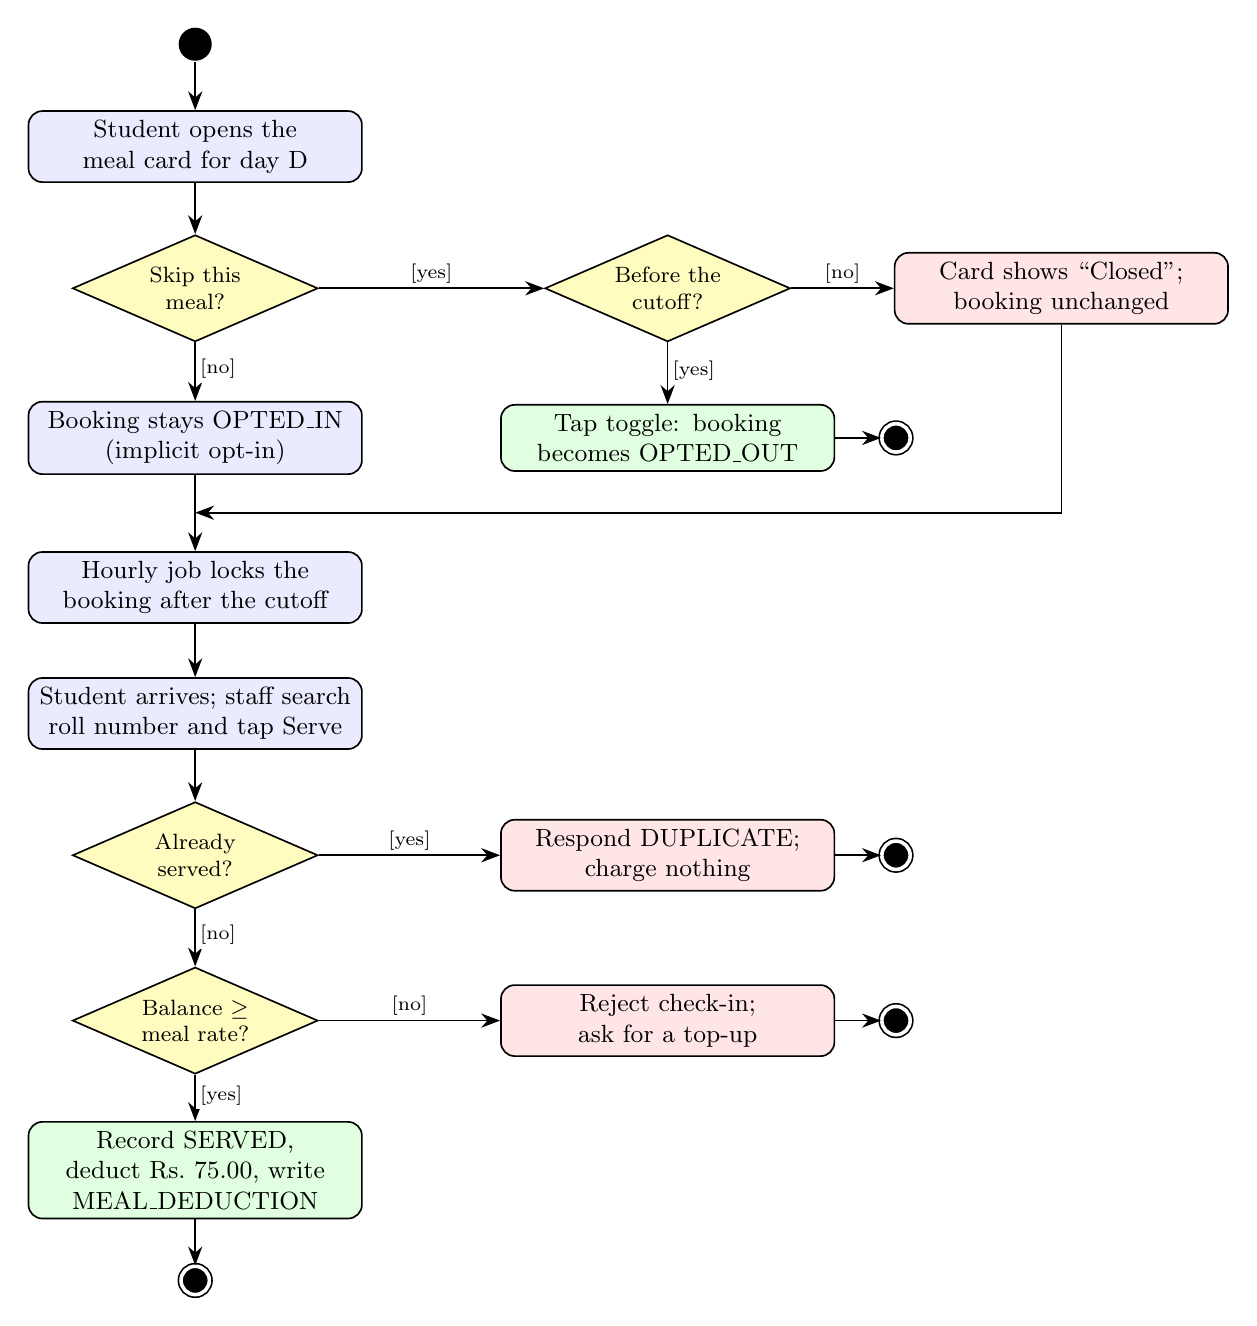
\begin{tikzpicture}[node distance=0.6cm]
  \node[startnode] (s) at (0,0) {};
  \node[act]  (a1) at (0,-1.3)  {Student opens the meal card for day D};
  \node[dec]  (d1) at (0,-3.1) {Skip this meal?};
  \node[dec]  (d2) at (6.0,-3.1) {Before the cutoff?};
  \node[actg] (a2) at (6.0,-5.0) {Tap toggle: booking becomes OPTED\_OUT};
  \node[endnode] (e1) at (8.9,-5.0) {};
  \node[actr] (a3) at (11.0,-3.1) {Card shows ``Closed''; booking unchanged};
  \node[act]  (a4) at (0,-5.0)  {Booking stays OPTED\_IN (implicit opt-in)};
  \node[act]  (a5) at (0,-6.9)  {Hourly job locks the booking after the cutoff};
  \node[act]  (a6) at (0,-8.5)  {Student arrives; staff search roll number and tap Serve};
  \node[dec]  (d3) at (0,-10.3)  {Already served?};
  \node[actr] (a7) at (6.0,-10.3) {Respond DUPLICATE; charge nothing};
  \node[endnode] (e2) at (8.9,-10.3) {};
  \node[dec]  (d4) at (0,-12.4) {Balance $\geq$ meal rate?};
  \node[actr] (a8) at (6.0,-12.4) {Reject check-in; ask for a top-up};
  \node[endnode] (e3) at (8.9,-12.4) {};
  \node[actg] (a9) at (0,-14.3) {Record SERVED, deduct Rs.~75.00, write MEAL\_DEDUCTION};
  \node[endnode] (e4) at (0,-15.7) {};
  \draw[->] (s) -- (a1);
  \draw[->] (a1) -- (d1);
  \draw[->] (d1) -- node[lbl, above]{[yes]} (d2);
  \draw[->] (d1) -- node[lbl, right, pos=0.45]{[no]} (a4);
  \draw[->] (d2) -- node[lbl, right, pos=0.45]{[yes]} (a2);
  \draw[->] (d2) -- node[lbl, above]{[no]} (a3);
  \draw[->] (a2) -- (e1);
  \draw[->] (a3.south) |- (0,-5.95);
  \draw[->] (a4) -- (a5);
  \draw[->] (a5) -- (a6);
  \draw[->] (a6) -- (d3);
  \draw[->] (d3) -- node[lbl, above]{[yes]} (a7);
  \draw[->] (a7) -- (e2);
  \draw[->] (d3) -- node[lbl, right, pos=0.45]{[no]} (d4);
  \draw[->] (d4) -- node[lbl, above]{[no]} (a8);
  \draw[->] (a8) -- (e3);
  \draw[->] (d4) -- node[lbl, right, pos=0.45]{[yes]} (a9);
  \draw[->] (a9) -- (e4);
\end{tikzpicture}}
\caption{Activity diagram for one meal, from opt-out to counter service}
\label{fig:activity}
\end{figure}

The swimlane diagram in Figure~\ref{fig:swimlane} distributes the semester-end
cashout over the four parties that take part in it. The mobile app only collects
the request and shows the outcome. The backend owns every rule: it resolves the
semester end date, checks the balance, and on approval re-checks the balance
inside the transaction that deducts it. The warden acts only on requests that
the backend has already accepted, and the database is written twice, once when
the request is created and once when it is approved.

\begin{figure}[H]
\centering
\resizebox{\textwidth}{!}{%
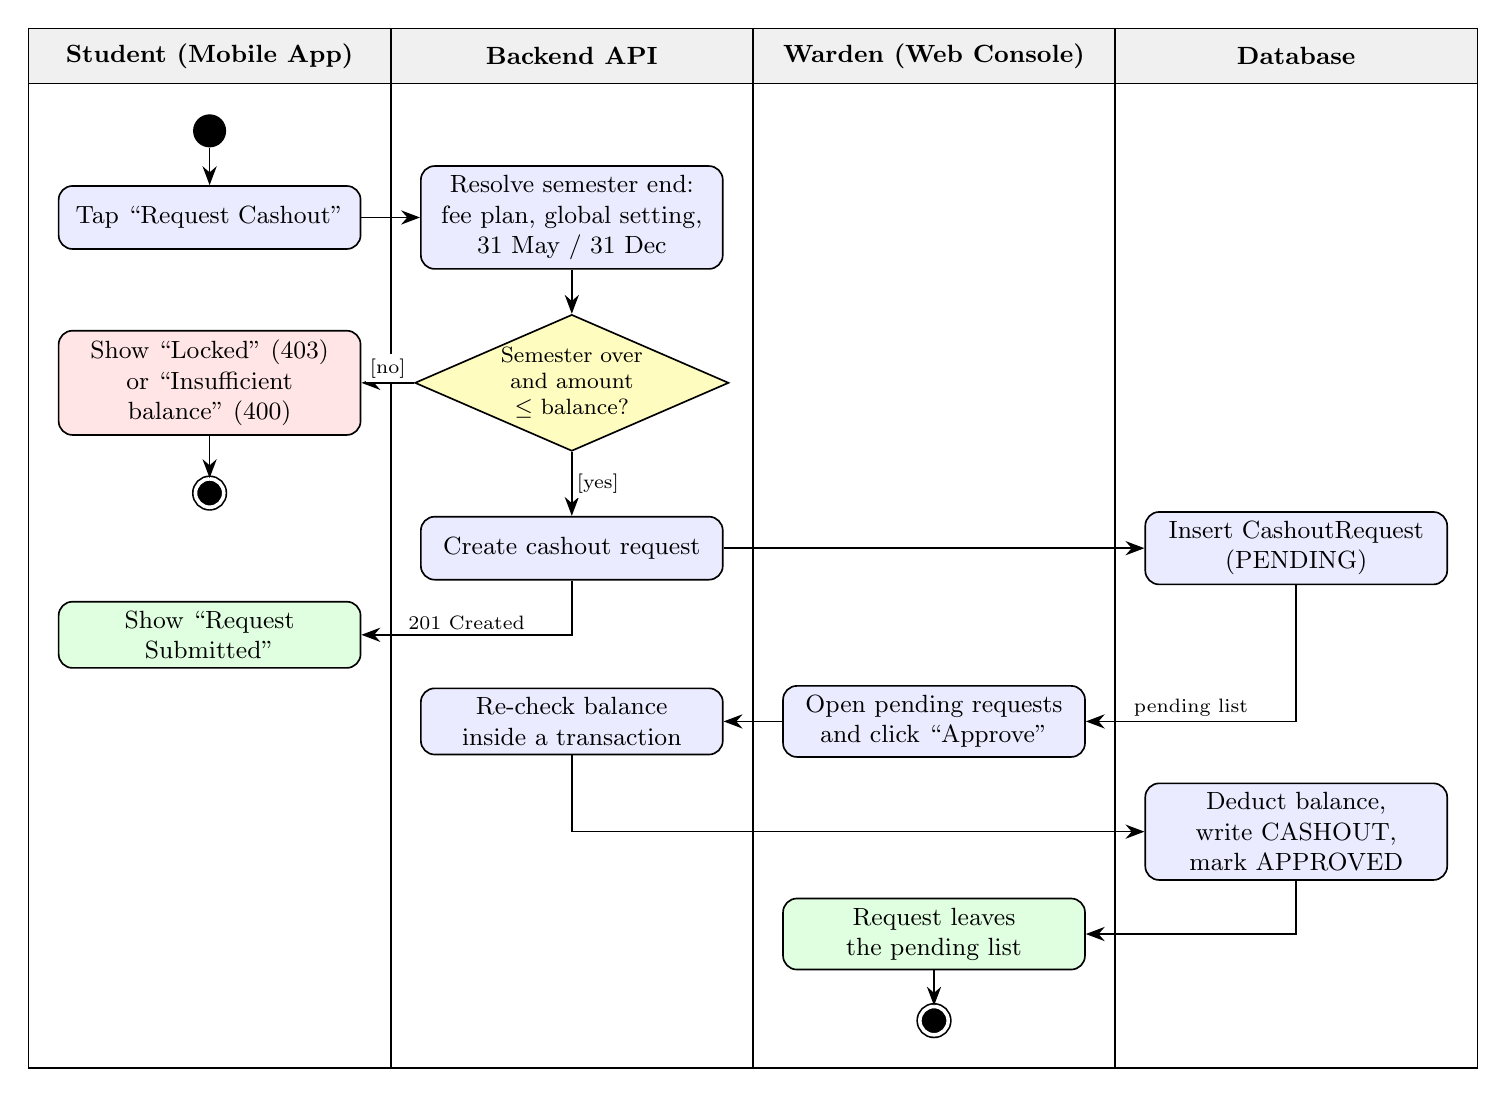
\begin{tikzpicture}
  % lanes
  \foreach \x/\t in {0/{Student (Mobile App)},4.6/{Backend API},9.2/{Warden (Web Console)},13.8/{Database}} {
    \draw (\x,0) rectangle ++(4.6,-13.2);
    \draw[fill=gray!12] (\x,0) rectangle ++(4.6,-0.7);
    \node[font=\bfseries\small] at ($(\x,0)+(2.3,-0.35)$) {\t};
  }
  \node[startnode] (s) at (2.3,-1.3) {};
  \node[act, text width=3.6cm] (s1) at (2.3,-2.4) {Tap ``Request Cashout''};
  \node[act, text width=3.6cm] (b1) at (6.9,-2.4) {Resolve semester end: fee plan, global setting, 31 May / 31 Dec};
  \node[dec] (bd) at (6.9,-4.5) {Semester over and amount $\leq$ balance?};
  \node[actr, text width=3.6cm] (se) at (2.3,-4.5) {Show ``Locked'' (403) or ``Insufficient balance'' (400)};
  \node[endnode] (e1) at (2.3,-5.9) {};
  \node[act, text width=3.6cm] (b2) at (6.9,-6.6) {Create cashout request};
  \node[act, text width=3.6cm] (db1) at (16.1,-6.6) {Insert CashoutRequest (PENDING)};
  \node[actg, text width=3.6cm] (s2) at (2.3,-7.7) {Show ``Request Submitted''};
  \node[act, text width=3.6cm] (w1) at (11.5,-8.8) {Open pending requests and click ``Approve''};
  \node[act, text width=3.6cm] (b3) at (6.9,-8.8) {Re-check balance inside a transaction};
  \node[act, text width=3.6cm] (db2) at (16.1,-10.2) {Deduct balance, write CASHOUT, mark APPROVED};
  \node[actg, text width=3.6cm] (w2) at (11.5,-11.5) {Request leaves the pending list};
  \node[endnode] (e2) at (11.5,-12.6) {};
  \draw[->] (s) -- (s1);
  \draw[->] (s1) -- (b1);
  \draw[->] (b1) -- (bd);
  \draw[->] (bd) -- node[lbl, above]{[no]} (se);
  \draw[->] (se) -- (e1);
  \draw[->] (bd) -- node[lbl, right]{[yes]} (b2);
  \draw[->] (b2) -- (db1);
  \draw[->] (b2.south) |- node[lbl, pos=0.75, above]{201 Created} (s2.east);
  \draw[->] (db1.south) |- node[lbl, pos=0.75, above]{pending list} (w1.east);
  \draw[->] (w1) -- (b3);
  \draw[->] (b3.south) |- (db2.west);
  \draw[->] (db2.south) |- (w2.east);
  \draw[->] (w2) -- (e2);
\end{tikzpicture}}
\caption{Swimlane diagram for requesting and approving a semester-end cashout}
\label{fig:swimlane}
\end{figure}

\subsection{Data Flow Diagrams (DFDs)}
\subsubsection{DFD Level 0}

The context diagram in Figure~\ref{fig:dfd0} treats Savoury as a single process.
Students supply registration details, opt-outs and cashout requests and receive
the menu, their meal status, balances and notices. Mess Staff send serve
requests and receive the roster and the result of each serve. Hostel Admins
supply menus, notices, top-ups and approvals and receive headcounts and pending
cashouts. The Super Admin supplies hostels, fee plans and staff accounts. The
Brevo service receives verification e-mail requests and returns a message id.

\begin{figure}[H]
\centering
\resizebox{\textwidth}{!}{%
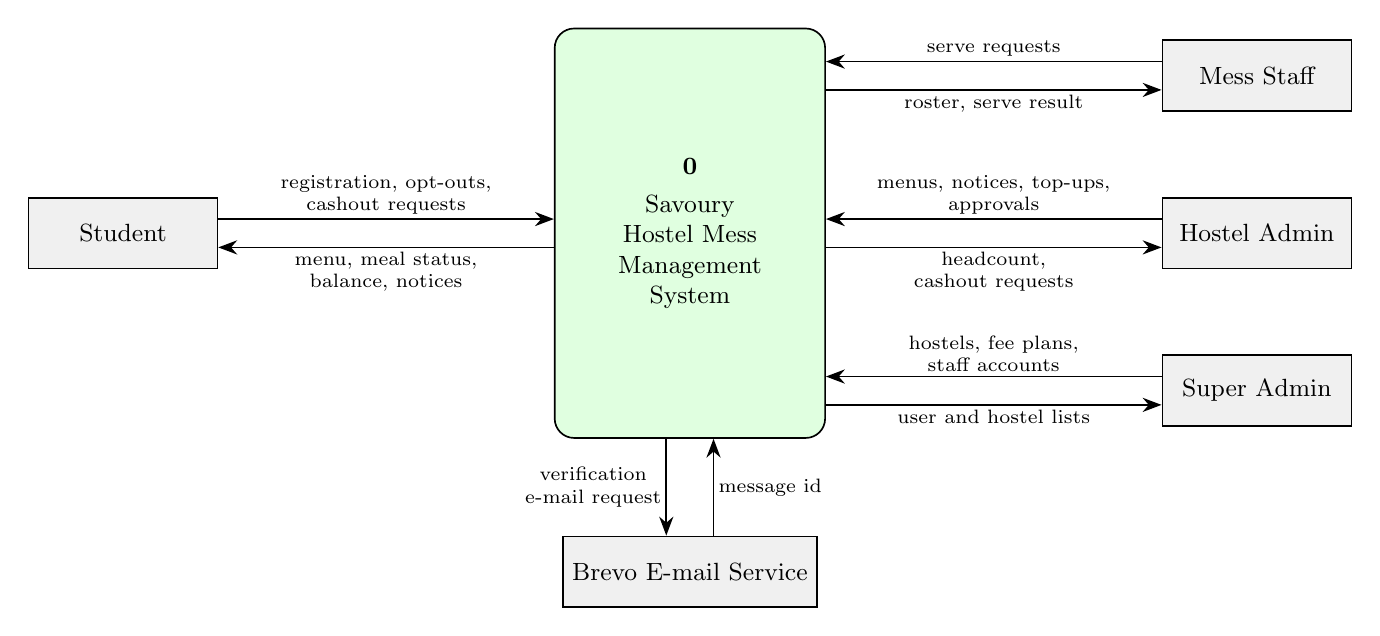
\begin{tikzpicture}
  \node[proc, fill=green!12, text width=3.2cm, minimum height=5.2cm] (sys) at (0,0)
       {\textbf{0}\\[0.3em]Savoury\\Hostel Mess\\Management\\System};
  \node[ent] (stu) at (-7.2,0) {Student};
  \node[ent] (msf) at (7.2,2.0) {Mess Staff};
  \node[ent] (adm) at (7.2,0) {Hostel Admin};
  \node[ent] (sad) at (7.2,-2.0) {Super Admin};
  \node[ent] (brv) at (0,-4.3) {Brevo E-mail Service};
  % student
  \draw[flow] ($(stu.east)+(0,0.18)$) -- node[lbl, above]{registration, opt-outs,\\cashout requests} ($(stu.east -| sys.west)+(0,0.18)$);
  \draw[flow] ($(stu.east -| sys.west)+(0,-0.18)$) -- node[lbl, below]{menu, meal status,\\balance, notices} ($(stu.east)+(0,-0.18)$);
  % staff
  \foreach \e/\i/\o in {msf/{serve requests}/{roster, serve result},
                        adm/{menus, notices, top-ups,\\approvals}/{headcount,\\cashout requests},
                        sad/{hostels, fee plans,\\staff accounts}/{user and hostel lists}} {
    \draw[flow] ($(\e.west)+(0,0.18)$) -- node[lbl, above]{\i} ($(\e.west -| sys.east)+(0,0.18)$);
    \draw[flow] ($(\e.west -| sys.east)+(0,-0.18)$) -- node[lbl, below]{\o} ($(\e.west)+(0,-0.18)$);
  }
  % brevo
  \draw[flow] ($(sys.south)+(-0.3,0)$) -- node[lbl, left]{verification\\e-mail request} ($(brv.north)+(-0.3,0)$);
  \draw[flow] ($(brv.north)+(0.3,0)$) -- node[lbl, right]{message id} ($(sys.south)+(0.3,0)$);
\end{tikzpicture}}
\caption{DFD Level 0 (context diagram)}
\label{fig:dfd0}
\end{figure}

\subsubsection{DFD Level 1}

Level 1 (Figure~\ref{fig:dfd1}) decomposes the system into seven processes and
six data stores. Authenticate User (1.0) reads and writes the Users \& Hostels
store and calls Brevo. Administer Hostels \& Users (2.0) maintains the same
store. Plan Meals (3.0) reads the meal configuration and menus and writes
bookings and opt-outs. Serve Meals (4.0) reads the booking, writes the
attendance and posts the deduction to the wallet ledger. Report Headcount (5.0)
reads bookings and attendance. Manage Wallets (6.0) handles top-ups and
cashouts against the ledger, and Publish Notices (7.0) writes notices that are
then delivered to the students of the same hostel.

\begin{figure}[H]
\centering
\resizebox{\textwidth}{!}{%
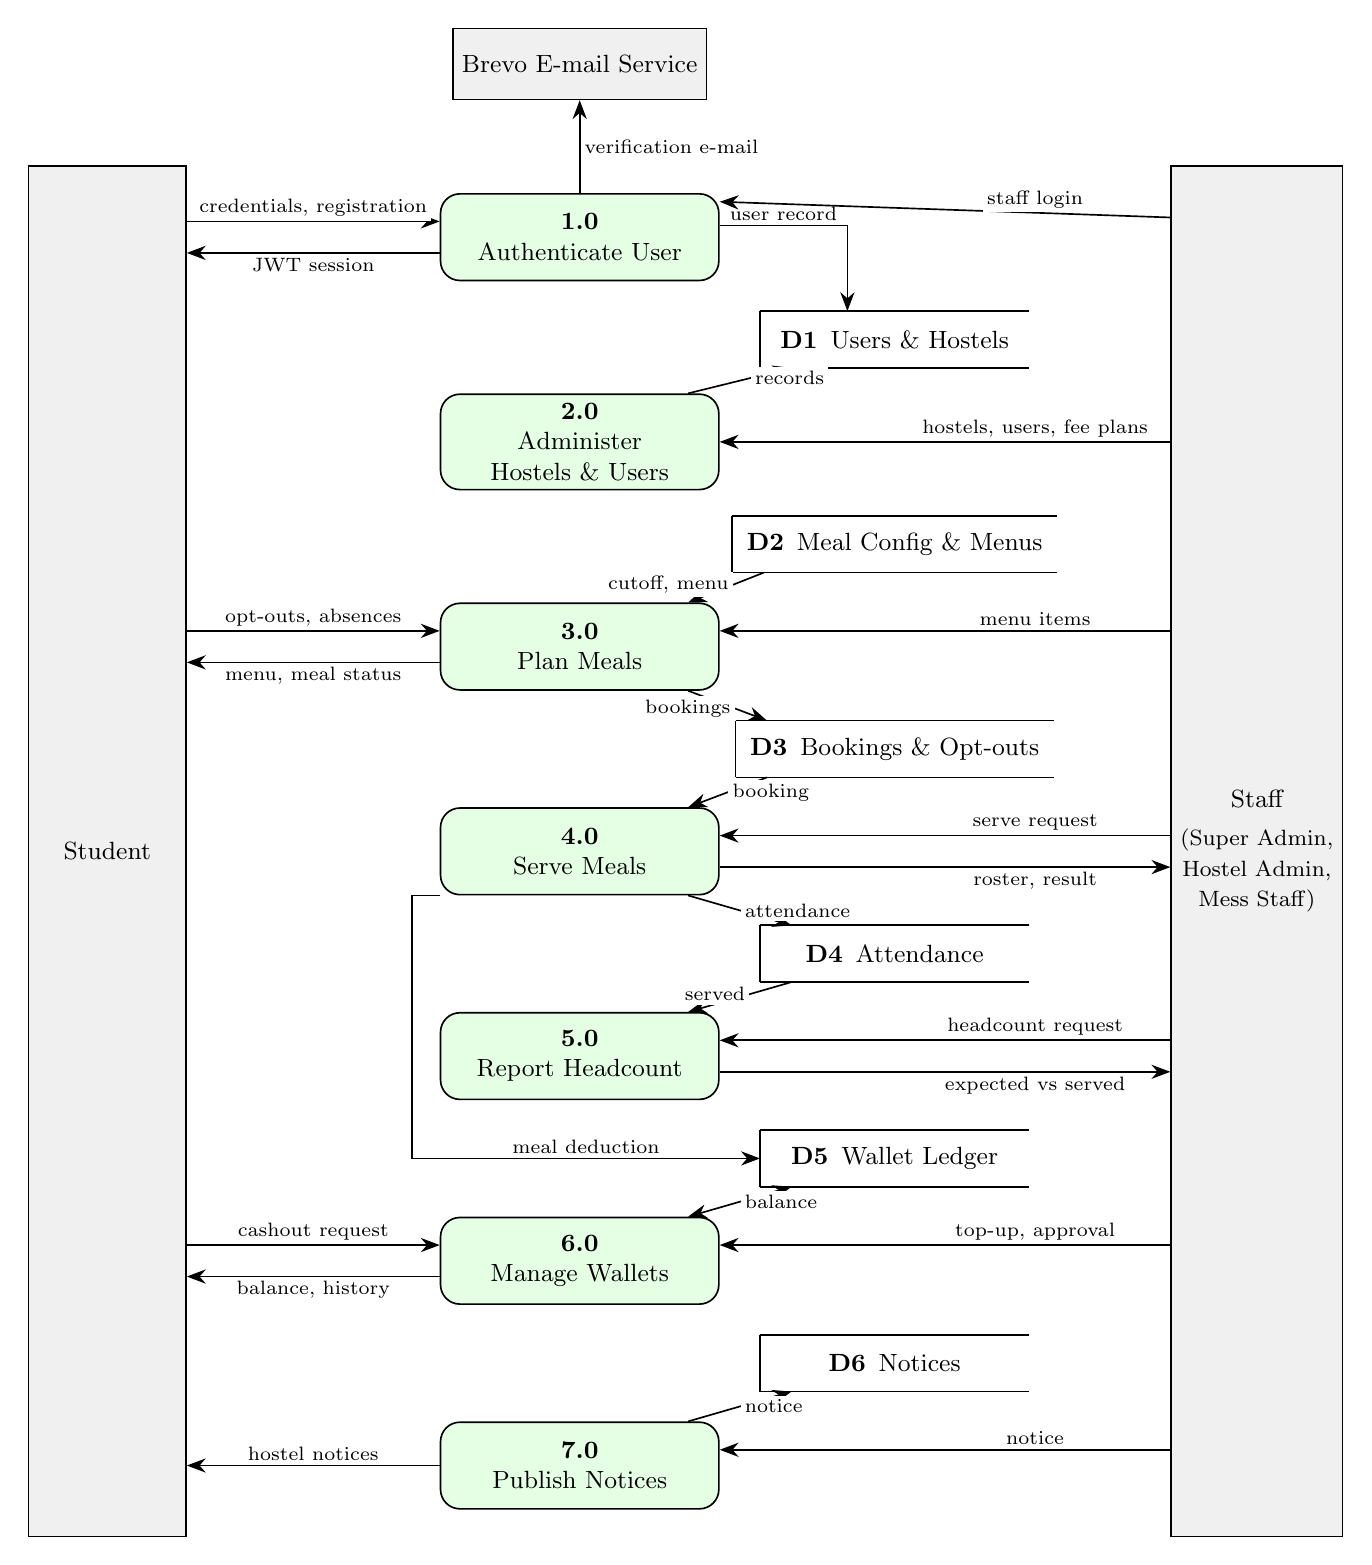
\begin{tikzpicture}
  % external entities (tall boxes)
  \node[ent, minimum width=2.0cm, minimum height=17.4cm] (stu) at (-0.4,-7.8) {Student};
  \node[ent, minimum width=2.0cm, minimum height=17.4cm, align=center] (stf) at (14.2,-7.8)
       {Staff\\[0.3em]\footnotesize (Super Admin,\\\footnotesize Hostel Admin,\\\footnotesize Mess Staff)};
  \node[ent] (brv) at (5.6,2.2) {Brevo E-mail Service};
  % processes
  \node[proc] (p1) at (5.6,0)     {\textbf{1.0}\\Authenticate User};
  \node[proc] (p2) at (5.6,-2.6)  {\textbf{2.0}\\Administer Hostels \& Users};
  \node[proc] (p3) at (5.6,-5.2)  {\textbf{3.0}\\Plan Meals};
  \node[proc] (p4) at (5.6,-7.8)  {\textbf{4.0}\\Serve Meals};
  \node[proc] (p5) at (5.6,-10.4) {\textbf{5.0}\\Report Headcount};
  \node[proc] (p6) at (5.6,-13.0) {\textbf{6.0}\\Manage Wallets};
  \node[proc] (p7) at (5.6,-15.6) {\textbf{7.0}\\Publish Notices};
  % data stores
  \node[store] (d1) at (9.6,-1.3)  {\textbf{D1}\enspace Users \& Hostels};
  \node[store] (d2) at (9.6,-3.9)  {\textbf{D2}\enspace Meal Config \& Menus};
  \node[store] (d3) at (9.6,-6.5)  {\textbf{D3}\enspace Bookings \& Opt-outs};
  \node[store] (d4) at (9.6,-9.1)  {\textbf{D4}\enspace Attendance};
  \node[store] (d5) at (9.6,-11.7) {\textbf{D5}\enspace Wallet Ledger};
  \node[store] (d6) at (9.6,-14.3) {\textbf{D6}\enspace Notices};
  % 1.0
  \draw[flow] ($(stu.east |- p1.west)+(0,0.2)$) -- node[lbl, above]{credentials, registration} ($(p1.west)+(0,0.2)$);
  \draw[flow] ($(p1.west)+(0,-0.2)$) -- node[lbl, below]{JWT session} ($(stu.east |- p1.west)+(0,-0.2)$);
  \draw[flow] (p1.north) -- node[lbl, right]{verification e-mail} (brv.south);
  \draw[flow] ($(p1.east)+(0,0.15)$) -| node[lbl, pos=0.25, above]{user record} ($(d1.north)+(-0.6,0)$);
  \draw[flow] ($(stf.west |- p1.east)+(0,0.25)$) -- node[lbl, above, pos=0.3]{staff login} ($(p1.east)+(0,0.45)$);
  % 2.0
  \draw[flow] ($(stf.west |- p2.east)$) -- node[lbl, above, pos=0.3]{hostels, users, fee plans} (p2.east);
  \draw[flow] ($(p2.north east)+(-0.4,0)$) -- node[lbl, right, pos=0.6]{records} ($(d1.south west)+(0.4,0)$);
  % 3.0
  \draw[flow] ($(stu.east |- p3.west)+(0,0.2)$) -- node[lbl, above]{opt-outs, absences} ($(p3.west)+(0,0.2)$);
  \draw[flow] ($(p3.west)+(0,-0.2)$) -- node[lbl, below]{menu, meal status} ($(stu.east |- p3.west)+(0,-0.2)$);
  \draw[flow] ($(stf.west |- p3.east)+(0,0.2)$) -- node[lbl, above, pos=0.3]{menu items} ($(p3.east)+(0,0.2)$);
  \draw[flow] ($(d2.south west)+(0.4,0)$) -- node[lbl, left, pos=0.4]{cutoff, menu} ($(p3.north east)+(-0.4,0)$);
  \draw[flow] ($(p3.south east)+(-0.4,0)$) -- node[lbl, left, pos=0.6]{bookings} ($(d3.north west)+(0.4,0)$);
  % 4.0
  \draw[flow] ($(stf.west |- p4.east)+(0,0.2)$) -- node[lbl, above, pos=0.3]{serve request} ($(p4.east)+(0,0.2)$);
  \draw[flow] ($(p4.east)+(0,-0.2)$) -- node[lbl, below, pos=0.7]{roster, result} ($(stf.west |- p4.east)+(0,-0.2)$);
  \draw[flow] ($(d3.south west)+(0.4,0)$) -- node[lbl, right, pos=0.5]{booking} ($(p4.north east)+(-0.4,0)$);
  \draw[flow] ($(p4.south east)+(-0.4,0)$) -- node[lbl, right, pos=0.5]{attendance} ($(d4.north west)+(0.4,0)$);
  \draw[flow] (p4.south west) -- ++(-0.35,0) |- node[lbl, pos=0.75, above]{meal deduction} (d5.west);
  % 5.0
  \draw[flow] ($(stf.west |- p5.east)+(0,0.2)$) -- node[lbl, above, pos=0.3]{headcount request} ($(p5.east)+(0,0.2)$);
  \draw[flow] ($(p5.east)+(0,-0.2)$) -- node[lbl, below, pos=0.7]{expected vs served} ($(stf.west |- p5.east)+(0,-0.2)$);
  \draw[flow] ($(d4.south west)+(0.4,0)$) -- node[lbl, left, pos=0.4]{served} ($(p5.north east)+(-0.4,0)$);
  % 6.0
  \draw[flow] ($(stu.east |- p6.west)+(0,0.2)$) -- node[lbl, above]{cashout request} ($(p6.west)+(0,0.2)$);
  \draw[flow] ($(p6.west)+(0,-0.2)$) -- node[lbl, below]{balance, history} ($(stu.east |- p6.west)+(0,-0.2)$);
  \draw[flow] ($(stf.west |- p6.east)+(0,0.2)$) -- node[lbl, above, pos=0.3]{top-up, approval} ($(p6.east)+(0,0.2)$);
  \draw[flow, <->] ($(d5.south west)+(0.4,0)$) -- node[lbl, right, pos=0.5]{balance} ($(p6.north east)+(-0.4,0)$);
  % 7.0
  \draw[flow] ($(stf.west |- p7.east)+(0,0.2)$) -- node[lbl, above, pos=0.3]{notice} ($(p7.east)+(0,0.2)$);
  \draw[flow] ($(p7.west)$) -- node[lbl, above]{hostel notices} (stu.east |- p7.west);
  \draw[flow] ($(p7.north east)+(-0.4,0)$) -- node[lbl, right, pos=0.5]{notice} ($(d6.south west)+(0.4,0)$);
\end{tikzpicture}}
\caption{DFD Level 1}
\label{fig:dfd1}
\end{figure}

\subsubsection{DFD Level 2}

Figure~\ref{fig:dfd2} expands process 4.0, where money moves. Process 4.1
authenticates the staff member and reloads their current role and hostel from
the Users store. Process 4.2 rejects a student of another hostel. Process 4.3
rejects a date other than today and a time outside the meal's check-in window.
Process 4.4 upserts the booking and rejects an opted-out student. Processes 4.5
to 4.7 run inside one database transaction: 4.5 inserts the attendance (a second
insert for the same booking violates the unique constraint and is reported as
\texttt{DUPLICATE}), 4.6 decrements the balance only if it covers the meal
rate, and 4.7 writes the ledger entry. A failure in 4.5 to 4.7 rolls back all
three.

\begin{figure}[H]
\centering
\resizebox{0.95\textwidth}{!}{%
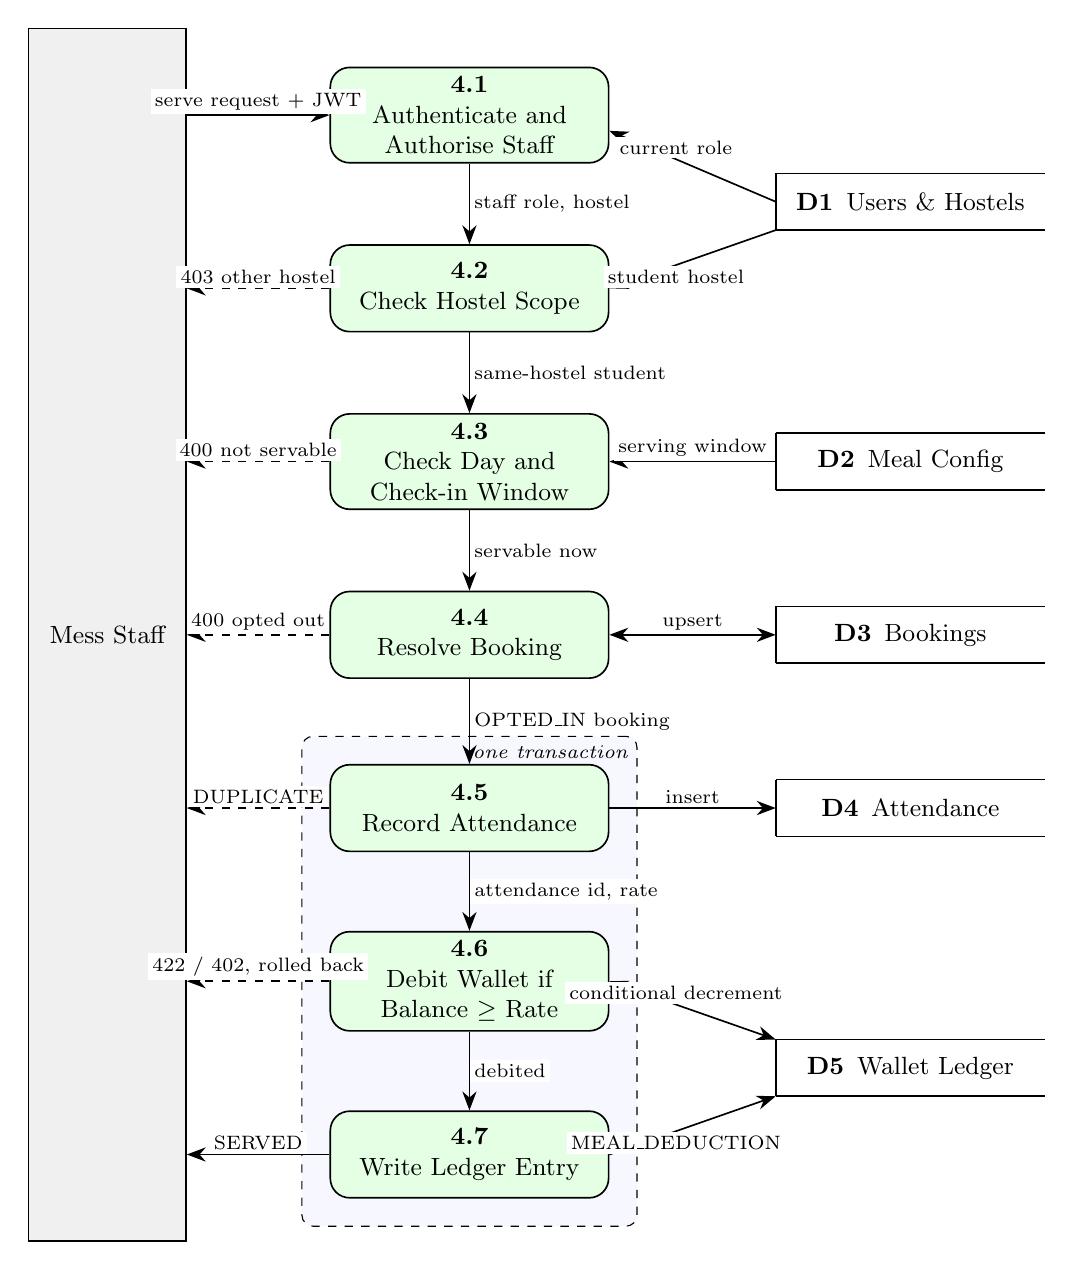
\begin{tikzpicture}
  \node[ent, minimum width=2.0cm, minimum height=15.4cm] (stf) at (-0.6,-6.6) {Mess Staff};
  \node[proc] (q1) at (4,0)     {\textbf{4.1}\\Authenticate and Authorise Staff};
  \node[proc] (q2) at (4,-2.2)  {\textbf{4.2}\\Check Hostel Scope};
  \node[proc] (q3) at (4,-4.4)  {\textbf{4.3}\\Check Day and Check-in Window};
  \node[proc] (q4) at (4,-6.6)  {\textbf{4.4}\\Resolve Booking};
  \node[proc] (q5) at (4,-8.8)  {\textbf{4.5}\\Record Attendance};
  \node[proc] (q6) at (4,-11.0) {\textbf{4.6}\\Debit Wallet if Balance $\geq$ Rate};
  \node[proc] (q7) at (4,-13.2) {\textbf{4.7}\\Write Ledger Entry};
  \node[store] (s1) at (9.6,-1.1)  {\textbf{D1}\enspace Users \& Hostels};
  \node[store] (s2) at (9.6,-4.4)  {\textbf{D2}\enspace Meal Config};
  \node[store] (s3) at (9.6,-6.6)  {\textbf{D3}\enspace Bookings};
  \node[store] (s4) at (9.6,-8.8)  {\textbf{D4}\enspace Attendance};
  \node[store] (s5) at (9.6,-12.1) {\textbf{D5}\enspace Wallet Ledger};
  \begin{scope}[on background layer]
    \node[draw, dashed, rounded corners, fill=blue!3, fit=(q5)(q6)(q7), inner sep=0.35cm,
          label={[font=\scriptsize\itshape, anchor=north east]north east:one transaction}] {};
  \end{scope}
  \draw[flow] ($(stf.east |- q1.west)$) -- node[lbl, above]{serve request + JWT} (q1.west);
  \draw[flow] (q1) -- node[lbl, right]{staff role, hostel} (q2);
  \draw[flow] (q2) -- node[lbl, right]{same-hostel student} (q3);
  \draw[flow] (q3) -- node[lbl, right]{servable now} (q4);
  \draw[flow] (q4) -- node[lbl, right]{OPTED\_IN booking} (q5);
  \draw[flow] (q5) -- node[lbl, right]{attendance id, rate} (q6);
  \draw[flow] (q6) -- node[lbl, right]{debited} (q7);
  \draw[flow] (s1.west) -- node[lbl, above, pos=0.6]{current role} ($(q1.east)+(0,-0.2)$);
  \draw[flow] (s1.south west) -- node[lbl, below, pos=0.6]{student hostel} (q2.east);
  \draw[flow] (s2.west) -- node[lbl, above]{serving window} (q3.east);
  \draw[flow, <->] (s3.west) -- node[lbl, above]{upsert} (q4.east);
  \draw[flow] (q5.east) -- node[lbl, above]{insert} (s4.west);
  \draw[flow, <->] (q6.east) -- node[lbl, above, pos=0.4]{conditional decrement} (s5.north west);
  \draw[flow] (q7.east) -- node[lbl, below, pos=0.4]{MEAL\_DEDUCTION} (s5.south west);
  % rejections back to staff
  \foreach \q/\t in {q2/{403 other hostel}, q3/{400 not servable}, q4/{400 opted out}} {
    \draw[flow, dashed] (\q.west) -- node[lbl, above]{\t} (\q.west -| stf.east);
  }
  \draw[flow, dashed] (q5.west) -- node[lbl, above]{DUPLICATE} (q5.west -| stf.east);
  \draw[flow, dashed] (q6.west) -- node[lbl, above]{422 / 402, rolled back} (q6.west -| stf.east);
  \draw[flow] (q7.west) -- node[lbl, above]{SERVED} (q7.west -| stf.east);
\end{tikzpicture}}
\caption{DFD Level 2: decomposition of process 4.0 Serve Meals}
\label{fig:dfd2}
\end{figure}

\subsection{Software Requirement Specification in IEEE Format}

This section follows the structure of IEEE Std 830 for software requirements
specifications. The full SRS is maintained in the repository as
\texttt{project-proposal/srs.tex}; the requirement numbers below are the same,
so the test cases in Section~\ref{sec:testing} trace directly to them.

\textbf{1. Introduction}

\textbf{1.1 Purpose.} This specification defines the requirements of Savoury,
version 1.0, for the developers, the course instructor, the hostel
administration and future maintainers. It states what the system must do and
the quality constraints it must meet, independent of the internal design
presented in later sections.

\textbf{1.2 Scope.} Savoury is a hostel mess management platform that lets
students opt out of meals before a configurable cutoff, gives the kitchen an
accurate headcount per meal, records who was actually served at the counter and
debits each student's prepaid wallet for the meals they take. It covers
authentication, hostel and role management, booking and opt-out, counter
attendance and billing, headcount, wallet and cashout, menus and notices. It
does not collect online payments, and guest meals, meal feedback and the audit
log are deferred.

\textbf{1.3 Definitions.} A \emph{hostel admin} is a Warden, Co-Warden or
Caretaker. \emph{Mess Staff} (role \texttt{COUNTER\_STAFF}) serve meals at the
counter. A \emph{student} includes Mess Committee members. A \emph{booking} is
the single record of one student's status (\texttt{OPTED\_IN},
\texttt{OPTED\_OUT} or \texttt{LOCKED}) for one meal on one date. \emph{Implicit
opt-in} means that a student with no booking row is assumed to eat. The
\emph{cutoff} is the instant after which a booking can no longer change. The
\emph{expected count} is the number of students minus those opted out. IST
denotes India Standard Time (UTC+5:30) and JWT a JSON Web Token.

\textbf{1.4 References.} IEEE Std 830-1998, Recommended Practice for Software
Requirements Specifications; the Savoury product requirements document and
project proposal; the Express, Prisma, React and Expo documentation; the Test
Case Template Doc:T\_01.

\textbf{1.5 Overview.} Part 2 describes the product in general terms and Part 3
lists the specific functional and non-functional requirements.

\textbf{2. Overall Description}

\textbf{2.1 Product perspective.} Savoury replaces the manual, paper-based mess
attendance and billing process. It is a new, self-contained client--server
product made of a REST backend with a PostgreSQL database, a student mobile app
and a staff web console. It depends on two external services: Supabase for the
managed PostgreSQL database and, optionally, Brevo for verification e-mail.

\textbf{2.2 Product functions.} At a high level the product authenticates users,
administers hostels and users, plans meals through bookings and opt-outs,
serves and bills meals, reports headcounts, manages wallets and publishes
notices. These functions correspond to processes 1.0 to 7.0 of the Level~1 DFD.

\textbf{2.3 User characteristics.} Students are hostel residents with ordinary
smartphone skills. Mess Staff work under time pressure at meal times and need
one search and one tap per student. Hostel admins use the console a few times
a day. The Super Admin is a technically capable system administrator.

\textbf{2.4 Constraints.} All meal times are configured and displayed in IST.
Registration is limited to the \texttt{@thapar.edu} domain. Staff accounts are
never self-registered. The system must run on free hosting tiers, so database
connections are scarce and polling intervals must stay modest.

\textbf{2.5 Assumptions and dependencies.} Each hostel has exactly one mess.
Students pay the mess through the institute's existing channel and a hostel
admin records the top-up. The counter device has a modern browser; the student
device runs Android or iOS.

\textbf{3. Specific Requirements}

\textbf{3.1 External interface requirements.} The user interfaces are the Expo
mobile app (Home, Opt-Out Calendar, Wallet, Notices, Profile) and the web
console (Check-In, Headcount, Menu, Users, Wallet, Hostels, Notices, Setup). The
software interface is a JSON REST API; every endpoint except setup,
registration, login, verification and \texttt{/health} requires a bearer JWT.
The backend talks to PostgreSQL through Prisma and to Brevo over HTTPS.

\textbf{3.2 Functional requirements.} Table~\ref{tab:fr} lists the functional
requirements of version 1.0.

\begin{longtable}{@{}L{1.4cm}L{13.4cm}@{}}
\caption{Functional requirements}\label{tab:fr}\\
\toprule
\textbf{ID} & \textbf{Requirement}\\
\midrule
\endfirsthead
\toprule
\textbf{ID} & \textbf{Requirement}\\
\midrule
\endhead
\bottomrule
\endfoot
\multicolumn{2}{@{}l}{\textit{Authentication and accounts}}\\
FR-1 & The system shall create the first Super Admin through a one-time setup endpoint and reject further setup attempts with HTTP 409.\\
FR-2 & A student shall self-register with a name, an \texttt{@thapar.edu} e-mail, a password of at least 6 characters, and an optional hostel, roll number, room number and 10-digit phone number. Self-registration shall only create Student accounts.\\
FR-3 & Login shall issue a signed JWT, valid for 7 days, carrying the user's id, role and hostel.\\
FR-4 & Every endpoint except setup, registration, login and the health check shall require a valid token, and the acting user's identity shall come only from the token.\\
FR-5 & Warden, Co-Warden, Caretaker and Mess Staff accounts shall be created by administrators only.\\
\multicolumn{2}{@{}l}{\textit{Hostels and role management}}\\
FR-6 & The Super Admin shall create, rename and delete hostels; creating a hostel shall also create its mess.\\
FR-7 & The Super Admin shall set a fee plan per hostel and semester, with a total fee and an optional semester end date.\\
FR-8 & The Super Admin shall create users of any role. Each hostel shall have at most one Warden and one Co-Warden (HTTP 409 for a second); Caretakers and Mess Staff are unlimited.\\
FR-9 & A Warden or Co-Warden shall create Mess Staff accounts for their own hostel only. A Caretaker shall not create any account.\\
FR-10 & A hostel admin shall not edit, change the role of, or delete a Warden, Co-Warden, Caretaker or Super Admin.\\
FR-11 & A hostel admin shall only switch a student between Student and Mess Committee. A Mess Staff account's role shall not be changed (HTTP 403).\\
FR-12 & A user shall not delete their own account (HTTP 400).\\
FR-13 & Every user other than the Super Admin shall see and act on data of their own hostel only.\\
\multicolumn{2}{@{}l}{\textit{Meal booking and opt-out}}\\
FR-14 & A student shall be treated as eating every meal unless they have opted out (implicit opt-in).\\
FR-15 & A student shall opt in to or out of a single meal on a given date, with at most one booking per student, meal and date.\\
FR-16 & Each meal's cutoff shall be computed from its configured IST cutoff time; if the cutoff time is later than the serving start, the cutoff falls on the previous day.\\
FR-17 & Changing a booking after its cutoff, or after it has been locked, shall be rejected with HTTP 400.\\
FR-18 & A student shall opt out of whole days across a date range in one request; meals past their cutoff shall be skipped and the number skipped reported.\\
FR-19 & A student shall cancel an opt-out for a date or date range, reopening only the meals still before their cutoff.\\
FR-20 & An hourly job shall mark open \texttt{OPTED\_IN} bookings as \texttt{LOCKED} once their cutoff has passed.\\
\multicolumn{2}{@{}l}{\textit{Counter attendance and billing}}\\
FR-21 & Mess Staff, Mess Committee members and hostel admins shall load the hostel roster for a meal and date with each student's booking status and served flag.\\
FR-22 & Marking a student served shall, in one transaction, record a \texttt{SERVED} attendance, deduct the per-meal rate from the wallet and write a \texttt{MEAL\_DEDUCTION} transaction.\\
FR-23 & A student who opted out of the meal shall not be marked served (HTTP 400).\\
FR-24 & Serving the same booking a second time shall record and charge nothing and report \texttt{DUPLICATE}.\\
FR-25 & Authorised staff shall record an override for a walk-in, with a non-empty reason, billed like a normal serve. Mess Staff shall not record overrides.\\
FR-26 & Staff shall serve or override only students of their own hostel (HTTP 403).\\
FR-27 & If the student has no wallet account, serving shall fail and record nothing.\\
\multicolumn{2}{@{}l}{\textit{Headcount}}\\
FR-28 & For a date, the system shall report per meal the total students, opted-out count, expected count, served count (\texttt{SERVED} plus \texttt{OVERRIDE}) and cutoff time, plus the total served.\\
FR-29 & The dashboard shall show each meal as Upcoming, Final, Active or Over, computed in IST, and refresh automatically.\\
FR-30 & Each meal's served percentage shall be served divided by expected, capped at 100\%, and 0\% when nobody is expected.\\
\multicolumn{2}{@{}l}{\textit{Wallet and cashout}}\\
FR-31 & A student shall view their wallet balance and a paginated transaction history.\\
FR-32 & A hostel admin shall top up the wallet of a student in their own hostel for a semester, creating the wallet if missing and recording a \texttt{TOPUP} transaction.\\
FR-33 & A student shall request a cashout only from the day after the semester ends (HTTP 403 before). The end date comes from the hostel's fee plan, else the global setting, else 31 May or 31 December.\\
FR-34 & A cashout request larger than the balance shall be rejected (HTTP 400).\\
FR-35 & A hostel admin shall approve or reject a pending cashout of their hostel; approval re-checks the balance, deducts it and records a \texttt{CASHOUT} transaction; a resolved request cannot be resolved again (HTTP 400).\\
FR-36 & The Super Admin shall set the global semester end date, readable by any signed-in user.\\
\multicolumn{2}{@{}l}{\textit{Menu and notices}}\\
FR-37 & Every user shall view the menu of their hostel's mess for a date range.\\
FR-38 & Mess Committee members and hostel admins shall create and update menu items, with at most one menu per mess, meal and date.\\
FR-39 & Mess Committee members and hostel admins shall post notices to their hostel, optionally targeted at one role.\\
FR-40 & A user shall see notices that are global or for their hostel, and untargeted or targeted at their role.\\
FR-41 & A Mess Committee member shall delete only their own notices; hostel admins and the Super Admin may delete any notice of their scope.\\
FR-42 & The mobile app shall detect new notices by polling the timestamp of the latest visible notice.\\
FR-43 & Expected versus served counts, and therefore attendance and wastage rates, shall be computable from stored data.\\
\end{longtable}

\textbf{3.3 Non-functional requirements.} \emph{Performance:} roster and
headcount queries use the composite indexes on bookings
(\texttt{mealTypeId, date, status}) and (\texttt{studentId, date}); the
headcount dashboard polls every 30 seconds and the check-in roster every 15
seconds so that open dashboards do not starve the connections used by
check-ins. \emph{Reliability:} attendance and wallet updates run in one
transaction, and unique constraints prevent duplicate bookings, duplicate
attendance and duplicate wallets. \emph{Security:} passwords are hashed with
bcrypt; JWTs are signed with HS256 and a secret that must be set, is checked
against known defaults and should be at least 32 characters; every request
reloads the user's current role and hostel from the database, and a password
change invalidates existing sessions through a password fingerprint in the
token; \texttt{helmet}, a CORS allow-list, a 1 MB body limit, a global limit of
2000 requests per 15 minutes per IP and a limit of 30 authentication requests
per 15 minutes protect the API; the web console sends a strict Content Security
Policy and HSTS. \emph{Usability:} every rejection carries a plain-language
message, and status badges and live counts guide staff during service.
\emph{Maintainability:} the backend is layered (routes, middleware, controllers,
services, Prisma), roles are defined once in \texttt{constants/roles.ts}, and
schema changes are Prisma migrations verified by CI. \emph{Portability:} the
backend runs on any platform with Node.js 22 and PostgreSQL, the console in any
modern browser, and the app on Android and iOS.

\subsection{User Stories and Story Cards}

User stories capture requirements from the users' perspective and were used to
plan the implementation iterations. Each card states the story, its priority and
its acceptance criteria.

\newcommand{\storycard}[4]{%
  \begin{tikzpicture}
    \node[card] (c) {\textbf{#1}\hfill\textit{Priority: #2}\\[0.35em]#3\\[0.35em]
      {\footnotesize\textbf{Acceptance:} #4}};
  \end{tikzpicture}}

\begin{center}
\storycard{US-01: Skip a meal}{High}{As a student, I want to opt out of a meal
from my phone so that I am not charged for food I will not eat.}{One tap before
the cutoff opts me out; after the cutoff the card shows ``Closed''.}\hfill
\storycard{US-02: Plan a trip}{High}{As a student going home, I want to opt out
of several days at once so that I do not have to toggle every meal.}{A date range
opts out all open meals and reports meals already closed.}\\[0.6em]
\storycard{US-03: Serve fast}{High}{As mess staff, I want to find a student by
roll number and serve with one tap so that the queue keeps moving.}{Search
narrows to one student; a served student leaves the waiting list.}\hfill
\storycard{US-04: Never double-charge}{High}{As a student, I want to be charged
at most once per meal so that my balance is always correct.}{A second serve of
the same meal reports DUPLICATE and deducts nothing.}\\[0.6em]
\storycard{US-05: Know how many will eat}{High}{As a warden, I want to see the
expected and served count for each meal so that the kitchen cooks the right
amount.}{Expected equals students minus opt-outs; counts update without a
reload.}\hfill
\storycard{US-06: Manage the balance}{Medium}{As a warden, I want to top up a
student's wallet so that their meals can be billed.}{The top-up appears on the
student's wallet with the new balance.}\\[0.6em]
\storycard{US-07: Get my money back}{Medium}{As a student, I want to cash out my
remaining balance at semester end so that I do not lose unused money.}{Cashout
is locked before the semester ends and needs warden approval.}\hfill
\storycard{US-08: Keep hostels apart}{High}{As a warden, I want to see only my
hostel's students and notices so that data stays private.}{Searches, rosters
and notices never include other hostels.}
\end{center}

% ============================================================
\clearpage
\section{Design Phase}
% ============================================================
\subsection{Class Diagram}

The design is presented through two class diagrams: one for the layered
structure of the backend and one for the persistent domain model.

\textbf{Backend layers.} Figure~\ref{fig:class1} shows the classes (TypeScript
modules) that handle a request. Every router depends on
\texttt{AuthMiddleware}, whose \texttt{authenticate} function verifies the JWT
with \texttt{Token} and reloads the user, and whose \texttt{authorizeRoles}
function compares the role against the groups defined once in \texttt{Roles}.
Controllers validate input with Zod schemas, apply hostel scoping and translate
results into HTTP responses; they hold no business rules of their own beyond
request checks such as \texttt{checkServableNow}. Services hold the rules:
\texttt{BookingService} and the opt-out controller rely on \texttt{Cutoff},
\texttt{AttendanceService} owns the serve-and-bill transaction, and
\texttt{CronService} locks bookings with the same \texttt{Cutoff} function, so
the cutoff rule exists in exactly one place. All data access goes through the
shared \texttt{PrismaClient}.

\begin{figure}[H]
\centering
\resizebox{\textwidth}{!}{%
\begin{tikzpicture}
  \node[cls=4.6cm] (rt) at (0,0) {\hfil\textit{\guillemotleft router\guillemotright}\hfil\\\hfil\textbf{ApiRouters}\hfil
    \nodepart{second}auth, menu, bookings, attendance, hostels, users, wallet, opt-outs, config, notices
    \nodepart{third}+ mount(app: Express)};
  \node[cls=4.6cm] (mw) at (6,0) {\hfil\textit{\guillemotleft middleware\guillemotright}\hfil\\\hfil\textbf{AuthMiddleware}\hfil
    \nodepart{second}
    \nodepart{third}+ authenticate(req, res, next)\\+ authorizeRoles(...roles)};
  \node[cls=4.6cm] (tk) at (12,0) {\hfil\textit{\guillemotleft utility\guillemotright}\hfil\\\hfil\textbf{Token}\hfil
    \nodepart{second}TOKEN\_TTL = 7d (HS256)
    \nodepart{third}+ signToken(user): string\\+ verifyToken(t): TokenPayload\\+ passwordFingerprint(hash)};
  \node[cls=4.6cm] (ro) at (12,-3.6) {\hfil\textit{\guillemotleft utility\guillemotright}\hfil\\\hfil\textbf{Roles}\hfil
    \nodepart{second}HOSTEL\_ADMIN\_ROLES\\MESS\_STAFF\_MANAGER\_ROLES\\STUDENT\_ROLES
    \nodepart{third}+ isHostelAdmin(role)\\+ canManageMessStaff(role)\\+ isStudentRole(role)};
  \node[cls=4.6cm] (ac) at (-1.5,-4.4) {\hfil\textit{\guillemotleft controller\guillemotright}\hfil\\\hfil\textbf{AttendanceController}\hfil
    \nodepart{second}- markServedSchema, overrideSchema
    \nodepart{third}+ getRoster(req, res)\\+ markServed(req, res)\\+ overrideAttendance(req, res)\\- checkServableNow(mealTypeId, date)};
  \node[cls=4.6cm] (bc) at (3.8,-4.4) {\hfil\textit{\guillemotleft controller\guillemotright}\hfil\\\hfil\textbf{BookingController}\hfil
    \nodepart{second}- toggleSchema
    \nodepart{third}+ getBookings(req, res)\\+ toggleBooking(req, res)\\+ getHeadcount(req, res)};
  \node[cls=4.6cm] (wc) at (-1.5,-8.4) {\hfil\textit{\guillemotleft controller\guillemotright}\hfil\\\hfil\textbf{WalletController}\hfil
    \nodepart{second}- topupSchema, cashoutSchema
    \nodepart{third}+ getMyWallet(), getMyTransactions()\\+ requestCashout(), topupWallet()\\+ getCashoutRequests()\\+ resolveCashoutRequest()};
  \node[cls=4.6cm] (oc) at (3.8,-8.4) {\hfil\textit{\guillemotleft controller\guillemotright}\hfil\\\hfil\textbf{OptOutController}\hfil
    \nodepart{second}
    \nodepart{third}+ getOptOuts(), setOptOuts()\\+ removeOptOut(), removeOptOutRange()};
  \node[cls=4.6cm] (as) at (-1.5,-12.6) {\hfil\textit{\guillemotleft service\guillemotright}\hfil\\\hfil\textbf{AttendanceService}\hfil
    \nodepart{second}
    \nodepart{third}+ getRoster(hostelId, mealTypeId, date)\\+ markServed(studentId, mealTypeId, date, staffId)\\+ createOverride(..., reason)};
  \node[cls=4.6cm] (bs) at (3.8,-12.6) {\hfil\textit{\guillemotleft service\guillemotright}\hfil\\\hfil\textbf{BookingService}\hfil
    \nodepart{second}
    \nodepart{third}+ getUserBookings(studentId, from, to)\\+ toggleBooking(studentId, mealTypeId, date, status)};
  \node[cls=4.6cm] (cs) at (9.2,-8.4) {\hfil\textit{\guillemotleft service\guillemotright}\hfil\\\hfil\textbf{CronService}\hfil
    \nodepart{second}schedule = ``0 * * * *''
    \nodepart{third}+ initCronJobs()};
  \node[cls=4.6cm] (cu) at (9.2,-12.6) {\hfil\textit{\guillemotleft utility\guillemotright}\hfil\\\hfil\textbf{Cutoff}\hfil
    \nodepart{second}IST\_OFFSET\_MINUTES = 330
    \nodepart{third}+ computeCutoffMoment(mealType, date): Date};
  \node[cls=4.6cm] (pc) at (3.8,-16.2) {\hfil\textit{\guillemotleft library\guillemotright}\hfil\\\hfil\textbf{PrismaClient}\hfil
    \nodepart{second}user, booking, attendance, walletAccount, walletTransaction, ...
    \nodepart{third}+ \$transaction(fn)\\+ findMany / upsert / updateMany()};
  \draw[dashed,->] (rt) -- node[lbl, above]{uses} (mw);
  \draw[dashed,->] (mw) -- node[lbl, above]{verifies with} (tk);
  \draw[dashed,->] (mw.south east) -- node[lbl, sloped, above]{checks} (ro.west);
  \draw[dashed,->] (rt.south) -- ++(0,-0.6) -| (ac.north);
  \draw[dashed,->] (rt.south) -- ++(0,-0.6) -| (bc.north);
  \draw[dashed,->] (ac) -- (as);
  \draw[dashed,->] (bc.south) -- ++(0,-0.5) -| ($(bs.north)+(1.2,0)$);
  \draw[dashed,->] (wc.south) -- ++(0,-0.4) -| ($(as.north)+(1.4,0)$);
  \draw[dashed,->] (oc.east) -| ($(cu.north)+(-1.4,0)$);
  \draw[dashed,->] (bs) -- node[lbl, above]{uses} (cu);
  \draw[dashed,->] (cs) -- node[lbl, right]{uses} (cu);
  \draw[dashed,->] (as.south) |- ($(pc.west)+(0,0.2)$);
  \draw[dashed,->] (bs) -- (pc);
  \draw[dashed,->] (cs.east) -- ++(0.5,0) |- ($(pc.east)+(0,0.2)$);
\end{tikzpicture}}
\caption{Class diagram 1: backend request-handling layers}
\label{fig:class1}
\end{figure}

\textbf{Domain model.} Figure~\ref{fig:class2} shows the entities stored in
PostgreSQL. A \texttt{Hostel} owns one \texttt{Mess}, its fee plans and its
users. A \texttt{User} holds at most one \texttt{Booking} per meal type and date;
the absence of a booking means the student is opted in. A booking has at most
one \texttt{Attendance}, which is why a second serve is detected by the database.
A student owns one \texttt{WalletAccount} per semester; each account owns its
\texttt{WalletTransaction} ledger, and deductions refer to the attendance that
caused them. \texttt{MealOptOut} marks a whole-day absence, \texttt{Notice}
belongs to a hostel and optionally targets a role, and \texttt{CashoutRequest}
records who resolved it. All child relationships cascade on delete.

\begin{figure}[H]
\centering
\resizebox{\textwidth}{!}{%
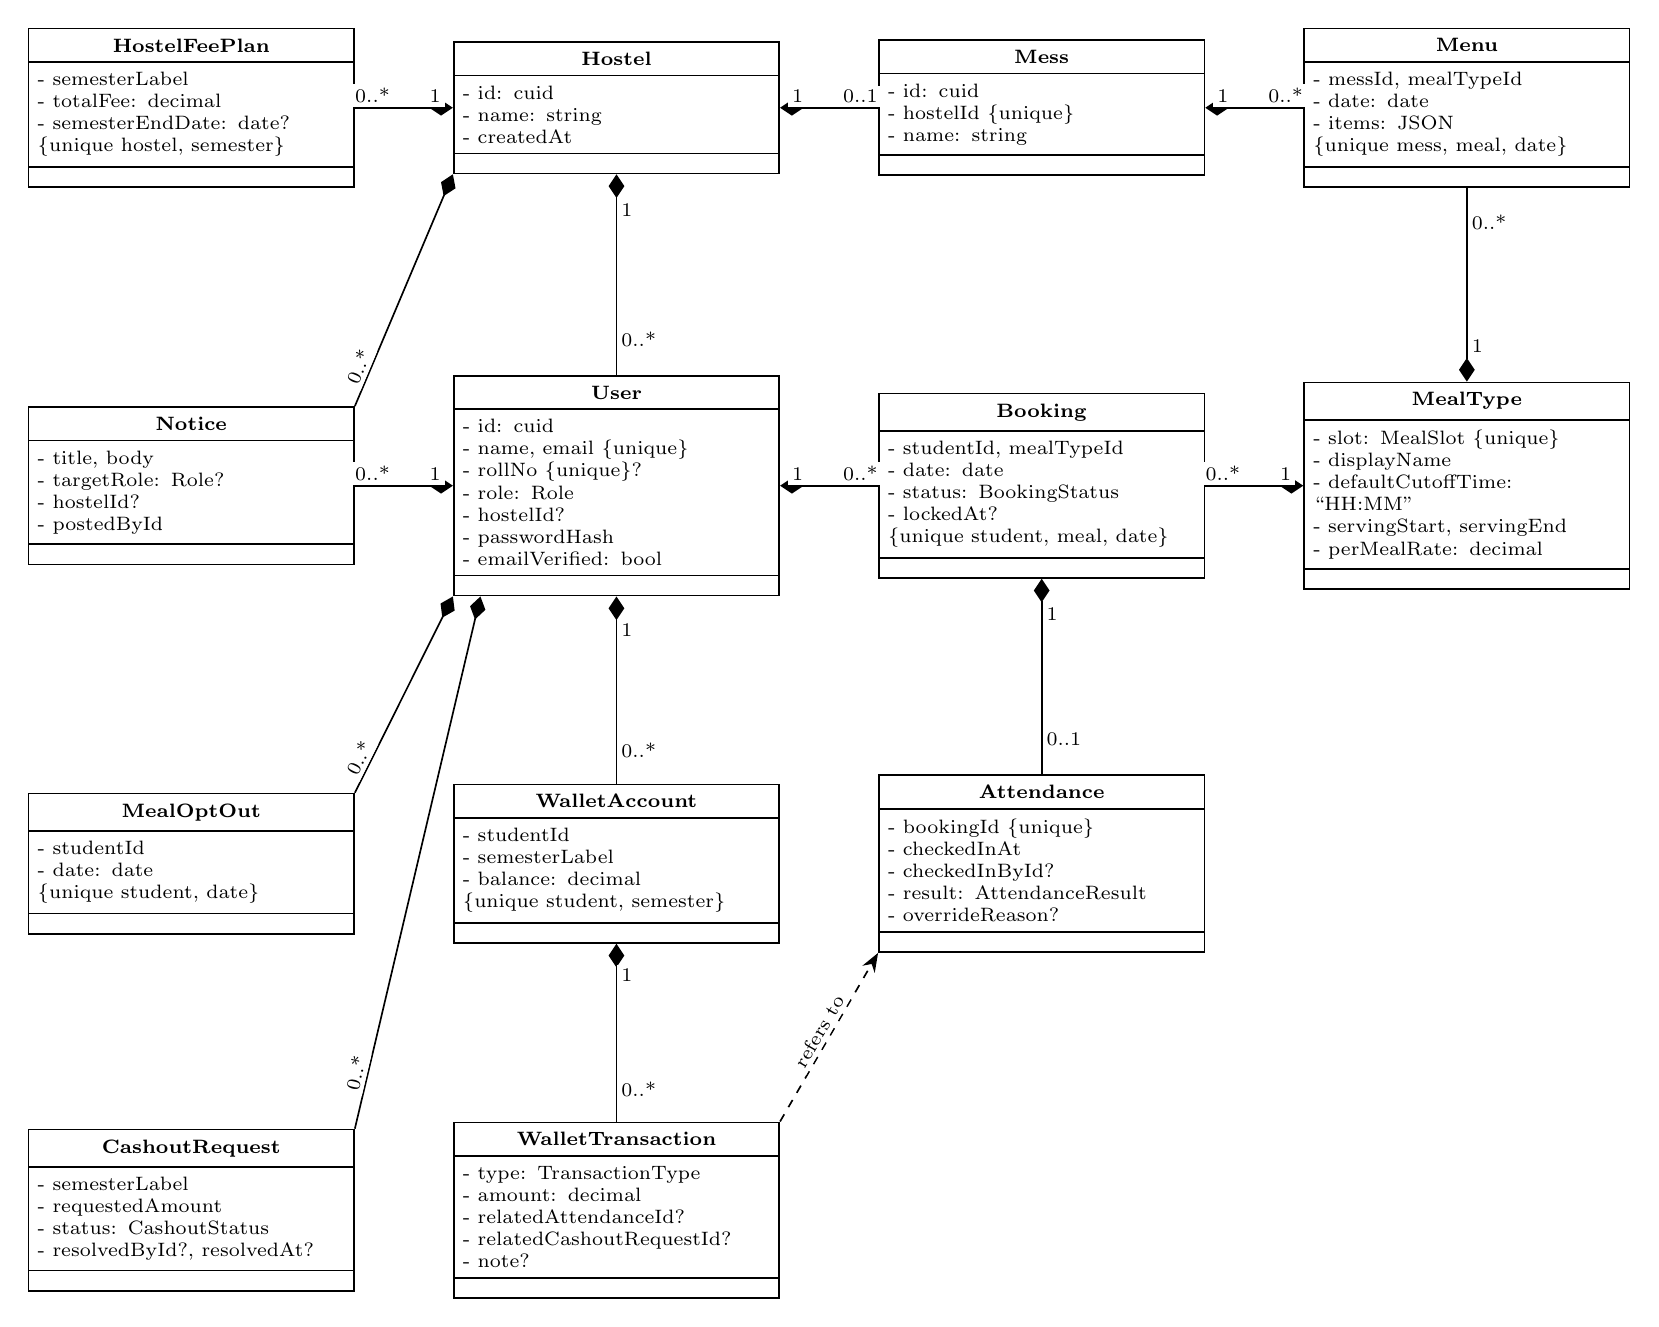
\begin{tikzpicture}
  \node[cls=3.9cm] (fp) at (0,0) {\hfil\textbf{HostelFeePlan}\hfil\nodepart{second}- semesterLabel\\- totalFee: decimal\\- semesterEndDate: date?\\\{unique hostel, semester\}\nodepart{third}};
  \node[cls=3.9cm] (ho) at (5.4,0) {\hfil\textbf{Hostel}\hfil\nodepart{second}- id: cuid\\- name: string\\- createdAt\nodepart{third}};
  \node[cls=3.9cm] (me) at (10.8,0) {\hfil\textbf{Mess}\hfil\nodepart{second}- id: cuid\\- hostelId \{unique\}\\- name: string\nodepart{third}};
  \node[cls=3.9cm] (mn) at (16.2,0) {\hfil\textbf{Menu}\hfil\nodepart{second}- messId, mealTypeId\\- date: date\\- items: JSON\\\{unique mess, meal, date\}\nodepart{third}};
  \node[cls=3.9cm] (nt) at (0,-4.8) {\hfil\textbf{Notice}\hfil\nodepart{second}- title, body\\- targetRole: Role?\\- hostelId?\\- postedById\nodepart{third}};
  \node[cls=3.9cm] (us) at (5.4,-4.8) {\hfil\textbf{User}\hfil\nodepart{second}- id: cuid\\- name, email \{unique\}\\- rollNo \{unique\}?\\- role: Role\\- hostelId?\\- passwordHash\\- emailVerified: bool\nodepart{third}};
  \node[cls=3.9cm] (bk) at (10.8,-4.8) {\hfil\textbf{Booking}\hfil\nodepart{second}- studentId, mealTypeId\\- date: date\\- status: BookingStatus\\- lockedAt?\\\{unique student, meal, date\}\nodepart{third}};
  \node[cls=3.9cm] (mt) at (16.2,-4.8) {\hfil\textbf{MealType}\hfil\nodepart{second}- slot: MealSlot \{unique\}\\- displayName\\- defaultCutoffTime: ``HH:MM''\\- servingStart, servingEnd\\- perMealRate: decimal\nodepart{third}};
  \node[cls=3.9cm] (oo) at (0,-9.6) {\hfil\textbf{MealOptOut}\hfil\nodepart{second}- studentId\\- date: date\\\{unique student, date\}\nodepart{third}};
  \node[cls=3.9cm] (wa) at (5.4,-9.6) {\hfil\textbf{WalletAccount}\hfil\nodepart{second}- studentId\\- semesterLabel\\- balance: decimal\\\{unique student, semester\}\nodepart{third}};
  \node[cls=3.9cm] (at) at (10.8,-9.6) {\hfil\textbf{Attendance}\hfil\nodepart{second}- bookingId \{unique\}\\- checkedInAt\\- checkedInById?\\- result: AttendanceResult\\- overrideReason?\nodepart{third}};
  \node[cls=3.9cm] (cr) at (0,-14.0) {\hfil\textbf{CashoutRequest}\hfil\nodepart{second}- semesterLabel\\- requestedAmount\\- status: CashoutStatus\\- resolvedById?, resolvedAt?\nodepart{third}};
  \node[cls=3.9cm] (wt) at (5.4,-14.0) {\hfil\textbf{WalletTransaction}\hfil\nodepart{second}- type: TransactionType\\- amount: decimal\\- relatedAttendanceId?\\- relatedCashoutRequestId?\\- note?\nodepart{third}};
  \tikzset{comp/.style={{Diamond[fill=black,length=3mm,width=2mm]}-}}
  \newcommand{\rel}[5][]{\draw[comp,#1] (#2) -- node[lbl, pos=0.18, above]{#4} node[lbl, pos=0.82, above]{#5} (#3);}
  \rel{ho}{fp}{1}{0..*}
  \rel{ho}{me}{1}{0..1}
  \rel{me}{mn}{1}{0..*}
  \draw[comp] (mt) -- node[lbl, pos=0.18, right]{1} node[lbl, pos=0.82, right]{0..*} (mn);
  \draw[comp] (ho) -- node[lbl, pos=0.18, right]{1} node[lbl, pos=0.82, right]{0..*} (us);
  \rel{us}{nt}{1}{0..*}
  \draw[comp] (ho.south west) -- node[lbl, pos=0.85, above, sloped]{0..*} (nt.north east);
  \rel{us}{bk}{1}{0..*}
  \rel{mt}{bk}{1}{0..*}
  \draw[comp] (bk) -- node[lbl, pos=0.18, right]{1} node[lbl, pos=0.82, right]{0..1} (at);
  \draw[comp] (us) -- node[lbl, pos=0.18, right]{1} node[lbl, pos=0.82, right]{0..*} (wa);
  \draw[comp] (us.south west) -- node[lbl, pos=0.85, above, sloped]{0..*} (oo.north east);
  \draw[comp] (wa) -- node[lbl, pos=0.18, right]{1} node[lbl, pos=0.82, right]{0..*} (wt);
  \draw[comp] ($(us.south west)+(0.35,0)$) -- node[lbl, pos=0.9, above, sloped]{0..*} (cr.north east);
  \draw[dashed,->] (wt.north east) -- node[lbl, above, sloped]{refers to} (at.south west);
\end{tikzpicture}}
\caption{Class diagram 2: domain model (Prisma schema; reserved GuestMeal, Feedback and
AuditLog entities omitted)}
\label{fig:class2}
\end{figure}

\subsection{Sequence Diagram}

\textbf{Serving a student.} Figure~\ref{fig:seq1} shows the messages exchanged
when Mess Staff serve a student. The check-in page posts to
\texttt{/attendance/mark-served}. The middleware reloads the staff member from
the database, the controller checks the student's hostel and the check-in
window, and the service upserts the booking. Inside the \texttt{alt} fragment
the first serve runs the transaction and returns \texttt{SERVED}; a repeated
serve hits the unique constraint on \texttt{Attendance.bookingId} (Prisma error
\texttt{P2002}), which the controller reports as HTTP 200 with the result
\texttt{DUPLICATE} so that a replayed offline serve is harmless.

\newcommand{\seqheads}[1]{%
  \foreach \x/\n in {#1} {
    \node[lifeline] at (\x,0) {\n};
    \draw[dashed, gray] (\x,-0.33) -- (\x,-\seqlen);
  }}
\newcommand{\msg}[4]{\draw[->] (#1,#3) -- node[lbl, above, font=\scriptsize]{#4} (#2,#3);}
\newcommand{\ret}[4]{\draw[->, dashed] (#1,#3) -- node[lbl, above, font=\scriptsize]{#4} (#2,#3);}
\newcommand{\self}[3]{\draw[->] (#1,#2) -- ++(0.5,0) -- ++(0,-0.35) node[lbl, right, font=\scriptsize, midway]{#3} -- ++(-0.5,0);}

\begin{figure}[H]
\centering
\resizebox{\textwidth}{!}{%
\begin{tikzpicture}
  \def\seqlen{14.6}
  \seqheads{0/Mess Staff,3/:CheckInPage,6.2/:AuthMiddleware,9.6/:AttendanceController,13/:AttendanceService,16.2/:Database}
  \msg{0}{3}{-1.0}{tap ``Serve''}
  \msg{3}{6.2}{-1.7}{POST /attendance/mark-served}
  \msg{6.2}{16.2}{-2.4}{load user (role, hostel, password fingerprint)}
  \ret{16.2}{6.2}{-3.0}{user row}
  \msg{6.2}{9.6}{-3.7}{next() with req.user}
  \msg{9.6}{16.2}{-4.4}{find student hostel}
  \ret{16.2}{9.6}{-5.0}{hostelId}
  \self{9.6}{-5.6}{checkServableNow()}
  \msg{9.6}{13}{-6.6}{markServed(studentId, mealTypeId, date, staffId)}
  \msg{13}{16.2}{-7.3}{upsert booking}
  \ret{16.2}{13}{-7.9}{booking (OPTED\_IN)}
  \draw (-0.6,-8.4) rectangle (16.8,-14.1);
  \node[draw, fill=white, font=\scriptsize\bfseries, anchor=north west] at (-0.6,-8.4) {alt};
  \node[font=\scriptsize, anchor=north west] at (0.2,-8.45) {[first serve of this booking]};
  \msg{13}{16.2}{-9.1}{\$transaction: attendance, debit, MEAL\_DEDUCTION}
  \ret{16.2}{13}{-9.7}{attendance}
  \ret{13}{9.6}{-10.3}{attendance}
  \ret{9.6}{3}{-10.9}{200 \{result: SERVED\}}
  \ret{3}{0}{-11.5}{student moves to recent check-ins}
  \draw[dashed] (-0.6,-12.0) -- (16.8,-12.0);
  \node[font=\scriptsize, anchor=north west] at (-0.5,-12.05) {[booking already has an attendance: P2002]};
  \ret{13}{9.6}{-12.8}{error 409}
  \ret{9.6}{3}{-13.5}{200 \{result: DUPLICATE\}}
\end{tikzpicture}}
\caption{Sequence diagram 1: serving a student at the counter}
\label{fig:seq1}
\end{figure}

\textbf{Opting out of a meal.} Figure~\ref{fig:seq2} shows how a toggle from the
mobile app is checked against the cutoff. The controller takes the student id
from the token, never from the body. The service loads the meal type, asks
\texttt{computeCutoffMoment} for the cutoff instant and compares it with the
current time. The \texttt{alt} fragment shows the two outcomes: before the cutoff
the single booking is upserted and the card shows ``Opted out''; after the
cutoff, or once the booking is locked, the request fails with HTTP 400 and the
card shows ``Closed''.

\begin{figure}[H]
\centering
\resizebox{\textwidth}{!}{%
\begin{tikzpicture}
  \def\seqlen{12.6}
  \seqheads{0/Student,3/:HomeScreen,6.4/:BookingController,9.8/:BookingService,13.2/:Cutoff,16.2/:Database}
  \msg{0}{3}{-1.0}{tap Lunch toggle}
  \msg{3}{6.4}{-1.7}{PUT /bookings/toggle}
  \self{6.4}{-2.3}{Zod parse; studentId from JWT}
  \msg{6.4}{9.8}{-3.3}{toggleBooking(studentId, mealTypeId, date, status)}
  \msg{9.8}{16.2}{-4.0}{find meal type}
  \ret{16.2}{9.8}{-4.6}{servingStart, defaultCutoffTime}
  \msg{9.8}{13.2}{-5.3}{computeCutoffMoment(mealType, date)}
  \ret{13.2}{9.8}{-5.9}{cutoff instant (UTC)}
  \draw (-0.6,-6.4) rectangle (16.8,-12.2);
  \node[draw, fill=white, font=\scriptsize\bfseries, anchor=north west] at (-0.6,-6.4) {alt};
  \node[font=\scriptsize, anchor=north west] at (0.2,-6.45) {[now $\leq$ cutoff and booking not locked]};
  \msg{9.8}{16.2}{-7.1}{upsert booking (student, meal, date)}
  \ret{16.2}{9.8}{-7.7}{booking}
  \ret{9.8}{6.4}{-8.3}{booking}
  \ret{6.4}{3}{-8.9}{200 OK}
  \ret{3}{0}{-9.5}{card shows ``Opted out''}
  \draw[dashed] (-0.6,-10.0) -- (16.8,-10.0);
  \node[font=\scriptsize, anchor=north west] at (-0.5,-10.05) {[cutoff passed or booking locked]};
  \ret{9.8}{6.4}{-10.8}{error 400}
  \ret{6.4}{3}{-11.4}{400 ``Cutoff time has passed for this meal''}
  \ret{3}{0}{-11.95}{card shows ``Closed''}
\end{tikzpicture}}
\caption{Sequence diagram 2: opting out of a meal before its cutoff}
\label{fig:seq2}
\end{figure}

\subsection{Collaboration Diagram}

Collaboration (communication) diagrams emphasise which objects are linked and the
numbered order of their messages.

\textbf{Wallet top-up.} In Figure~\ref{fig:collab1} the wallet page sends message
1 to the authentication middleware, which authenticates the warden (1.1) and
checks that the role is a hostel admin (1.2) before handing over to the wallet
controller (1.3). The controller loads the target student to check that it is a
student of the same hostel (1.3.1) and then runs one transaction that finds or
creates the semester wallet, increments the balance and writes the
\texttt{TOPUP} entry (1.3.2). The new balance returns to the page as message 1.4.

\begin{figure}[H]
\centering
\resizebox{0.95\textwidth}{!}{%
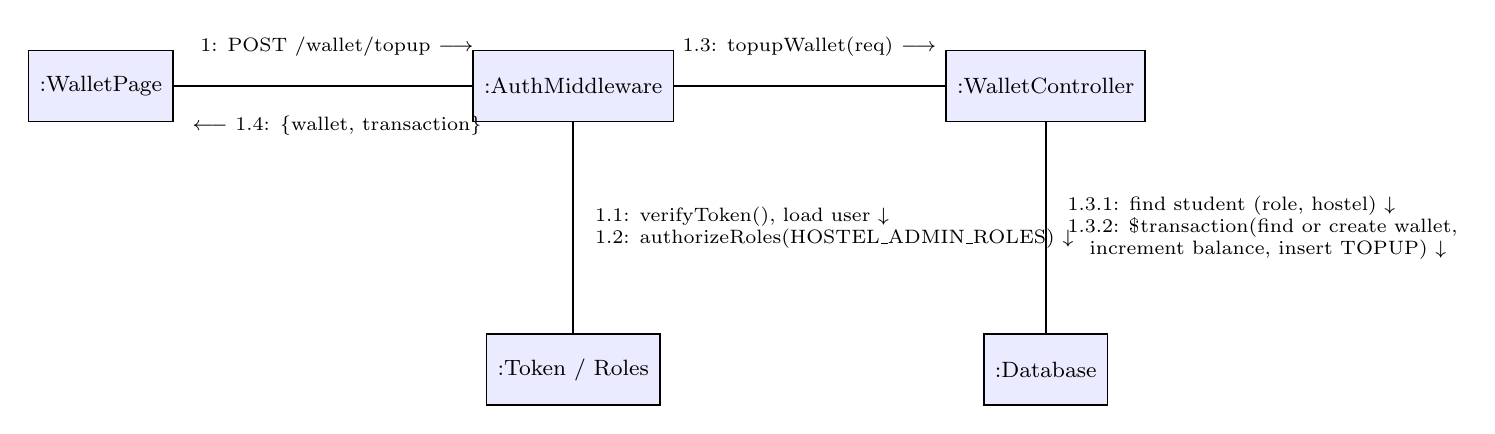
\begin{tikzpicture}
  \node[lifeline, minimum height=0.9cm] (wp) at (0,0) {:WalletPage};
  \node[lifeline, minimum height=0.9cm] (am) at (6,0) {:AuthMiddleware};
  \node[lifeline, minimum height=0.9cm] (wc) at (12,0) {:WalletController};
  \node[lifeline, minimum height=0.9cm] (db) at (12,-3.6) {:Database};
  \node[lifeline, minimum height=0.9cm] (tk) at (6,-3.6) {:Token / Roles};
  \draw (wp) -- (am); \draw (am) -- (wc); \draw (wc) -- (db); \draw (am) -- (tk);
  \node[font=\scriptsize, above] at (3,0.25) {1: POST /wallet/topup $\longrightarrow$};
  \node[font=\scriptsize, below] at (3,-0.25) {$\longleftarrow$ 1.4: \{wallet, transaction\}};
  \node[font=\scriptsize, align=left, right] at (6.15,-1.8) {1.1: verifyToken(), load user $\downarrow$\\1.2: authorizeRoles(HOSTEL\_ADMIN\_ROLES) $\downarrow$};
  \node[font=\scriptsize, above] at (9,0.25) {1.3: topupWallet(req) $\longrightarrow$};
  \node[font=\scriptsize, align=left, right] at (12.15,-1.8) {1.3.1: find student (role, hostel) $\downarrow$\\1.3.2: \$transaction(find or create wallet,\\\quad increment balance, insert TOPUP) $\downarrow$};
\end{tikzpicture}}
\caption{Collaboration diagram 1: topping up a student's wallet}
\label{fig:collab1}
\end{figure}

\textbf{Registration with e-mail verification.} In Figure~\ref{fig:collab2} the
registration screen passes the form to the authentication context (1), which
posts it to the authentication controller (1.1). The controller asks the
authentication service to create the student (1.1.1); the service hashes the
password and inserts the user (1.1.1.1) and then asks the verification service
to send the link (1.1.1.2). The verification service stores only the SHA-256
hash of the token (1.1.1.2.1) and calls the Brevo API (1.1.1.2.2). The token and
user return to the context (1.2), which stores them for later requests.

\begin{figure}[H]
\centering
\resizebox{\textwidth}{!}{%
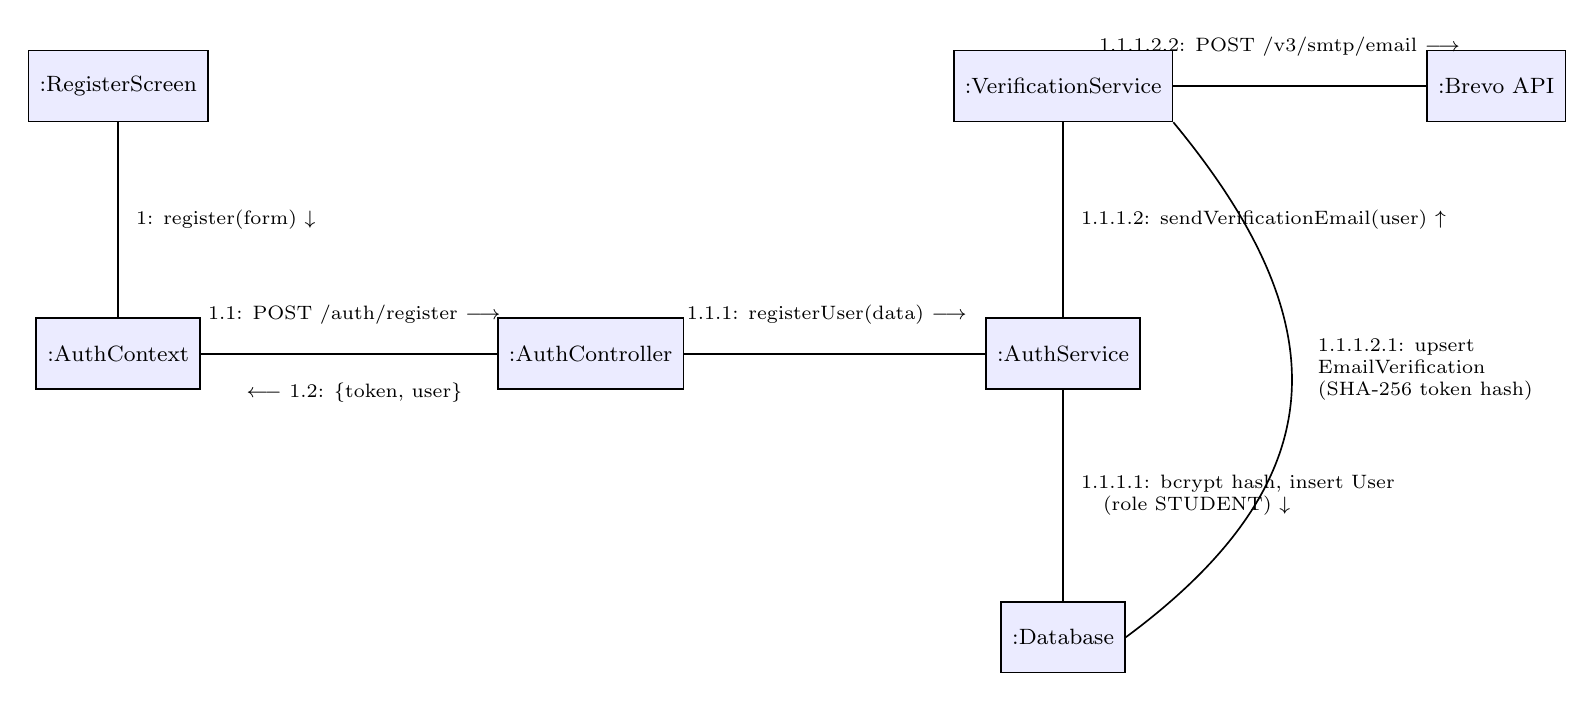
\begin{tikzpicture}
  \node[lifeline, minimum height=0.9cm] (rs) at (0,0) {:RegisterScreen};
  \node[lifeline, minimum height=0.9cm] (ax) at (0,-3.4) {:AuthContext};
  \node[lifeline, minimum height=0.9cm] (ac) at (6,-3.4) {:AuthController};
  \node[lifeline, minimum height=0.9cm] (as) at (12,-3.4) {:AuthService};
  \node[lifeline, minimum height=0.9cm] (vs) at (12,0) {:VerificationService};
  \node[lifeline, minimum height=0.9cm] (db) at (12,-7.0) {:Database};
  \node[lifeline, minimum height=0.9cm] (bv) at (17.5,0) {:Brevo API};
  \draw (rs) -- (ax); \draw (ax) -- (ac); \draw (ac) -- (as); \draw (as) -- (vs);
  \draw (as) -- (db); \draw (vs) -- (bv);
  \draw (vs.south east) .. controls (15.5,-3) and (15.5,-5) .. (db.east);
  \node[font=\scriptsize, right] at (0.1,-1.7) {1: register(form) $\downarrow$};
  \node[font=\scriptsize, above] at (3,-3.15) {1.1: POST /auth/register $\longrightarrow$};
  \node[font=\scriptsize, below] at (3,-3.65) {$\longleftarrow$ 1.2: \{token, user\}};
  \node[font=\scriptsize, above] at (9,-3.15) {1.1.1: registerUser(data) $\longrightarrow$};
  \node[font=\scriptsize, align=left, right] at (12.1,-5.2) {1.1.1.1: bcrypt hash, insert User\\\quad(role STUDENT) $\downarrow$};
  \node[font=\scriptsize, align=left, right] at (12.1,-1.7) {1.1.1.2: sendVerificationEmail(user) $\uparrow$};
  \node[font=\scriptsize, above] at (14.75,0.25) {1.1.1.2.2: POST /v3/smtp/email $\longrightarrow$};
  \node[font=\scriptsize, align=left] at (16.6,-3.6) {1.1.1.2.1: upsert\\EmailVerification\\(SHA-256 token hash)};
\end{tikzpicture}}
\caption{Collaboration diagram 2: registering a student with e-mail verification}
\label{fig:collab2}
\end{figure}

\subsection{State Chart Diagrams}

\textbf{Booking lifecycle.} Figure~\ref{fig:state1} models the status of one
student's booking for one meal. Every student starts in the implicit opted-in
state, in which no row exists. Opting out creates the row as
\texttt{OPTED\_OUT}; opting back in moves it to \texttt{OPTED\_IN}. Both
transitions are guarded by the cutoff. When the hourly job runs after the cutoff,
an \texttt{OPTED\_IN} booking becomes \texttt{LOCKED}; an \texttt{OPTED\_OUT}
booking keeps its status and can no longer change. Serving a student who has no
row first creates an \texttt{OPTED\_IN} booking with \texttt{lockedAt} set, and
every serve ends in the Served state, after which further serves are reported
as duplicates.

\begin{figure}[H]
\centering
\resizebox{\textwidth}{!}{%
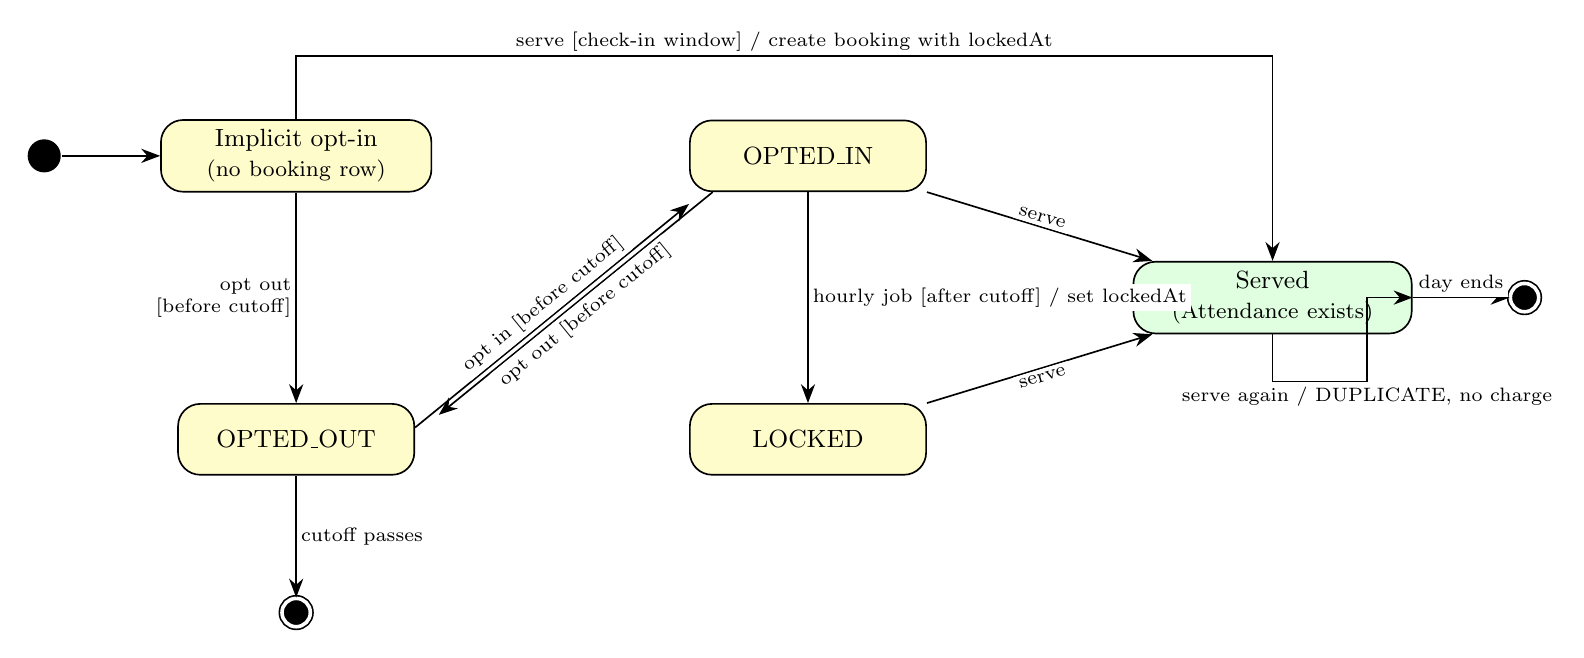
\begin{tikzpicture}
  \node[startnode] (i) at (-3.2,0) {};
  \node[st, text width=3.2cm] (im) at (0,0) {Implicit opt-in\\\footnotesize(no booking row)};
  \node[st] (in) at (6.5,0) {OPTED\_IN};
  \node[st] (out) at (0,-3.6) {OPTED\_OUT};
  \node[st] (lk) at (6.5,-3.6) {LOCKED};
  \node[stg, text width=3.3cm] (sv) at (12.4,-1.8) {Served\\\footnotesize(Attendance exists)};
  \node[endnode] (f1) at (0,-5.8) {};
  \node[endnode] (f2) at (15.6,-1.8) {};
  \draw[->] (i) -- (im);
  \draw[->] (im) -- node[lbl, left, align=right]{opt out\\{[before cutoff]}} (out);
  \draw[->] ([yshift=0.15cm]out.east) -- node[lbl, above, sloped]{opt in [before cutoff]} ([yshift=-0.15cm]in.south west);
  \draw[->] ([xshift=0.3cm]in.south west) -- node[lbl, below, sloped]{opt out [before cutoff]} ([yshift=-0.15cm, xshift=0.3cm]out.north east);
  \draw[->] (in) -- node[lbl, right]{hourly job [after cutoff] / set lockedAt} (lk);
  \draw[->] (im.north) -- ++(0,0.8) -| node[lbl, pos=0.25, above]{serve [check-in window] / create booking with lockedAt} (sv.north);
  \draw[->] (in) -- node[lbl, above, sloped]{serve} (sv);
  \draw[->] (lk) -- node[lbl, below, sloped]{serve} (sv);
  \draw[->] (out) -- node[lbl, right]{cutoff passes} (f1);
  \draw[->] (sv) -- node[lbl, above]{day ends} (f2);
  \draw[->] (sv.south) -- ++(0,-0.6) -- ++(1.2,0) node[lbl, below]{serve again / DUPLICATE, no charge} |- (sv.east);
\end{tikzpicture}}
\caption{State chart 1: booking lifecycle for one student, meal and date}
\label{fig:state1}
\end{figure}

\textbf{Cashout request.} Figure~\ref{fig:state2} shows the cashout request. A
request is created as \texttt{PENDING} only after the semester-end and balance
guards pass. A hostel admin moves it to \texttt{APPROVED}, which deducts the
balance, or to \texttt{REJECTED}, which leaves it untouched. Both are final; a
second resolution is refused. \texttt{PAID} exists in the schema for a later
step in which the actual bank transfer is recorded, and is not used in
version~1.0.

\begin{figure}[H]
\centering
\resizebox{0.9\textwidth}{!}{%
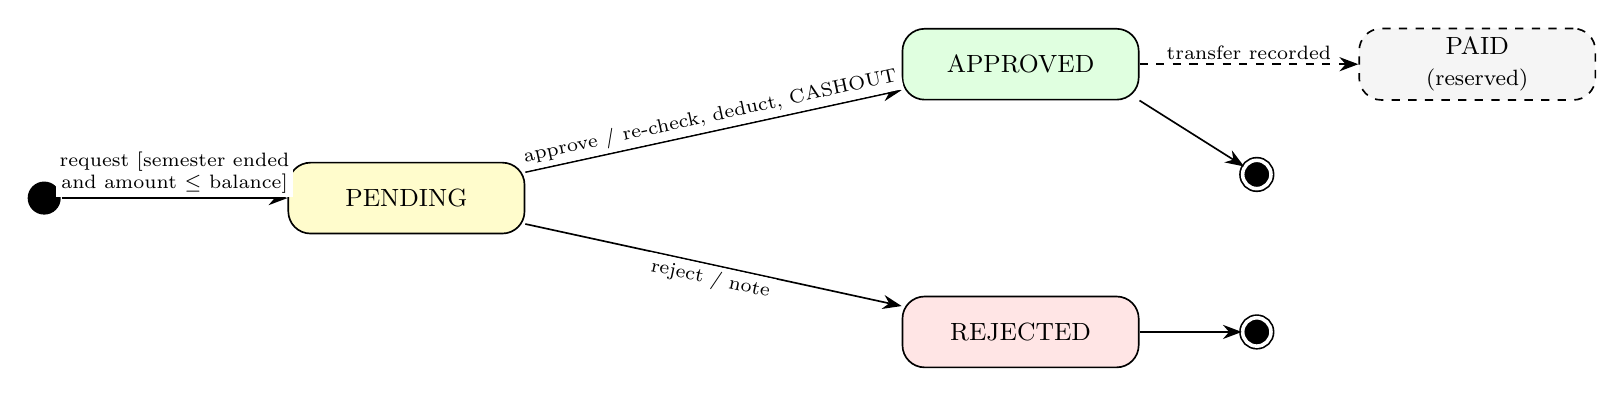
\begin{tikzpicture}
  \node[startnode] (i) at (-4.6,0) {};
  \node[st] (pd) at (0,0) {PENDING};
  \node[stg] (ap) at (7.8,1.7) {APPROVED};
  \node[str] (rj) at (7.8,-1.7) {REJECTED};
  \node[st, dashed, fill=gray!8] (pa) at (13.6,1.7) {PAID\\\footnotesize(reserved)};
  \node[endnode] (f1) at (10.8,-1.7) {};
  \node[endnode] (f2) at (10.8,0.3) {};
  \draw[->] (i) -- node[lbl, above, align=center]{request [semester ended\\and amount $\leq$ balance]} (pd);
  \draw[->] (pd) -- node[lbl, above, sloped]{approve / re-check, deduct, CASHOUT} (ap);
  \draw[->] (pd) -- node[lbl, below, sloped]{reject / note} (rj);
  \draw[->, dashed] (ap) -- node[lbl, above]{transfer recorded} (pa);
  \draw[->] (ap.south east) -- (f2);
  \draw[->] (rj) -- (f1);
\end{tikzpicture}}
\caption{State chart 2: cashout request}
\label{fig:state2}
\end{figure}

\textbf{Headcount meal badge.} Figure~\ref{fig:state3} models the badge shown on
each meal card of the dashboard for today. It is computed from the current IST
time: a meal is Upcoming until its cutoff, Final between the cutoff and the start
of serving, Active during the serving window and Over afterwards. Over takes
priority, so a meal never returns to an earlier state on the same day. For
tomorrow's view only Upcoming and Final can occur.

\begin{figure}[H]
\centering
\resizebox{\textwidth}{!}{%
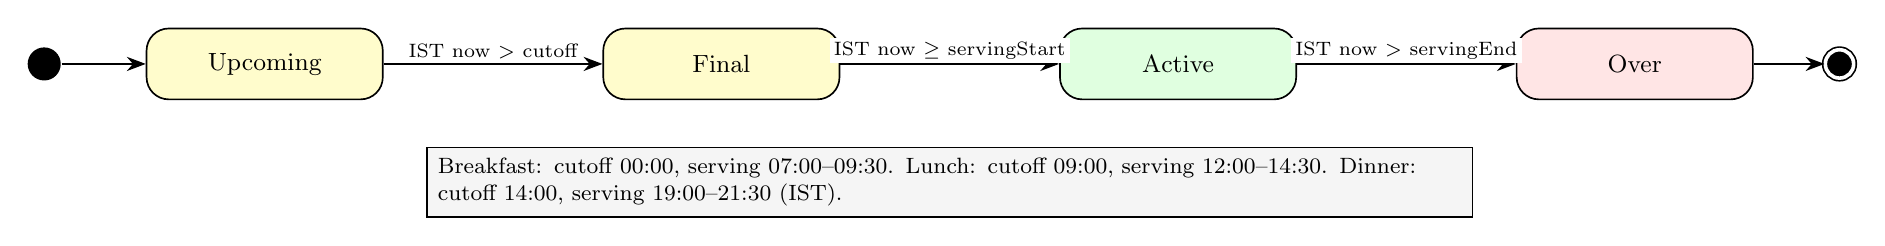
\begin{tikzpicture}
  \node[startnode] (i) at (-2.8,0) {};
  \node[st] (up) at (0,0) {Upcoming};
  \node[st] (fi) at (5.8,0) {Final};
  \node[stg] (ac) at (11.6,0) {Active};
  \node[str] (ov) at (17.4,0) {Over};
  \node[endnode] (f) at (20.0,0) {};
  \draw[->] (i) -- (up);
  \draw[->] (up) -- node[lbl, above]{IST now $>$ cutoff} (fi);
  \draw[->] (fi) -- node[lbl, above]{IST now $\geq$ servingStart} (ac);
  \draw[->] (ac) -- node[lbl, above]{IST now $>$ servingEnd} (ov);
  \draw[->] (ov) -- (f);
  \node[note, text width=13cm] at (8.7,-1.5) {Breakfast: cutoff 00:00, serving 07:00--09:30.
    Lunch: cutoff 09:00, serving 12:00--14:30. Dinner: cutoff 14:00, serving 19:00--21:30 (IST).};
\end{tikzpicture}}
\caption{State chart 3: headcount status badge of a meal}
\label{fig:state3}
\end{figure}

% ============================================================
\clearpage
\section{Implementation}
% ============================================================

The system is written in TypeScript end to end. The backend uses Node.js 22,
Express 4, Prisma 5 over PostgreSQL, Zod 3 for validation, bcrypt and
\texttt{jsonwebtoken} for authentication, \texttt{helmet} and
\texttt{express-rate-limit} for hardening and \texttt{node-cron} for the
booking-lock job. The web console uses React 19, Vite 8, React Router 7,
TanStack Query 5 and axios. The mobile app uses Expo SDK 57, React Native 0.86,
Expo Router, TanStack Query 5 and \texttt{expo-secure-store} for the session
token. All source code is under \texttt{code/}: \texttt{backend-api/},
\texttt{web/} and \texttt{mobile/}. Database changes are Prisma migrations
under \texttt{backend-api/prisma/migrations/}, and the seed script creates the
three meal types with their IST serving windows, cutoffs and the Rs.~75.00
rate.

\subsection{Component Diagrams}

Figure~\ref{fig:component} shows the software components and their
dependencies. Both clients follow the same pattern: screens or pages use
TanStack Query hooks, which call an axios API client that attaches the bearer
token held by an authentication context. The web check-in page adds an offline
queue stored in \texttt{localStorage} that replays serves when the network
returns. The only connection between the clients and the backend is the REST
interface over HTTPS. Inside the backend, routers depend on the authentication
middleware and on controllers; controllers depend on services; services use the
cutoff utility, the mailer and the Prisma client. The cron scheduler reuses the
cutoff utility and Prisma. Prisma talks to PostgreSQL on Supabase and the mailer
to the Brevo API.

\begin{figure}[H]
\centering
\resizebox{\textwidth}{!}{%
\begin{tikzpicture}[node distance=0.5cm, comp/.append style={text width=3.2cm}]
  % mobile
  \node[comp] (ms) at (0,0.2)    {\guillemotleft component\guillemotright\\Screens (Home, Opt-Out, Wallet, Notices, Profile)};
  \node[comp] (mq) at (0,-2.2) {\guillemotleft component\guillemotright\\Query hooks (useBookings, useToggleBooking, ...)};
  \node[comp] (ma) at (0,-4.6) {\guillemotleft component\guillemotright\\API client and AuthContext (SecureStore)};
  % web
  \node[comp] (wp) at (7,0)    {\guillemotleft component\guillemotright\\Pages (Check-In, Headcount, Users, Wallet, ...)};
  \node[comp] (wo) at (10.6,0) {\guillemotleft component\guillemotright\\Offline check-in queue (localStorage)};
  \node[comp] (wq) at (7,-2.2) {\guillemotleft component\guillemotright\\TanStack Query hooks};
  \node[comp] (wa) at (7,-4.6) {\guillemotleft component\guillemotright\\API client and AuthContext};
  % backend
  \node[comp] (rt) at (3.5,-8.2)  {\guillemotleft component\guillemotright\\API Routers (10 + /health)};
  \node[comp] (am) at (0,-8.2)    {\guillemotleft component\guillemotright\\Auth Middleware (JWT, roles)};
  \node[comp] (ct) at (7,-8.2)    {\guillemotleft component\guillemotright\\Controllers (Zod, hostel scope)};
  \node[comp] (sv) at (7,-10.6)    {\guillemotleft component\guillemotright\\Domain Services};
  \node[comp] (cr) at (10.6,-10.6) {\guillemotleft component\guillemotright\\Cron Scheduler (hourly lock)};
  \node[comp] (cu) at (3.5,-10.6)  {\guillemotleft component\guillemotright\\Cutoff utility (IST)};
  \node[comp] (ml) at (10.6,-13.0){\guillemotleft component\guillemotright\\Mailer};
  \node[comp] (pr) at (7,-13.0)   {\guillemotleft component\guillemotright\\Prisma Client};
  \node[comp] (tk) at (0,-10.6)    {\guillemotleft component\guillemotright\\Token and Roles};
  % external
  \node[comp, fill=gray!10] (db) at (7,-15.6) {\guillemotleft database\guillemotright\\PostgreSQL (Supabase)};
  \node[comp, fill=gray!10, dashed] (bv) at (15.0,-13.0) {\guillemotleft external\guillemotright\\Brevo e-mail API};
  % frames
  \begin{scope}[on background layer]
    \node[draw, rounded corners, fill=gray!4, fit=(ms)(mq)(ma), inner sep=0.35cm, label={[font=\bfseries\small]above:Mobile App (Expo)}] {};
    \node[draw, rounded corners, fill=gray!4, fit=(wp)(wo)(wq)(wa), inner sep=0.35cm, label={[font=\bfseries\small]above:Web Console (React + Vite)}] {};
    \node[draw, rounded corners, fill=gray!4, fit=(rt)(am)(ct)(sv)(cr)(cu)(ml)(pr)(tk), inner sep=0.35cm, label={[font=\bfseries\small]above:Backend API (Express)}] {};
  \end{scope}
  \tikzset{dep/.style={dashed,->}}
  \draw[dep] (ms) -- (mq); \draw[dep] (mq) -- (ma);
  \draw[dep] (wp) -- (wq); \draw[dep] (wq) -- (wa); \draw[dep] (wp) -- (wo);
  \draw[dep] (wo.south) |- (wa.east);
  \draw[dep] (ma.south) -- ++(0,-1.2) -| node[lbl, pos=0.25, above]{REST / JSON over HTTPS} ($(rt.north)+(-0.4,0)$);
  \draw[dep] (wa.south) -- ++(0,-1.2) -| ($(rt.north)+(0.4,0)$);
  \draw[dep] (rt) -- (am); \draw[dep] (rt) -- (ct); \draw[dep] (ct) -- (sv);
  \draw[dep] (am) -- (tk);
  \draw[dep] (sv) -- (cu); \draw[dep] (sv) -- (pr); \draw[dep] (sv) -- (ml);
  \draw[dep] (cr) -- (pr); \draw[dep] (cr.north) -- ++(0,0.45) -| ($(cu.north)+(0.5,0)$);
  \draw[dep] (am.south west) -- ++(-0.4,0) |- ($(pr.west)+(0,-0.2)$);
  \draw[dep] (pr) -- node[lbl, right]{SQL over TLS} (db);
  \draw[dep] (ml) -- node[lbl, above]{HTTPS} (bv);
\end{tikzpicture}}
\caption{Component diagram}
\label{fig:component}
\end{figure}

\subsection{Deployment Diagrams}

Figure~\ref{fig:deployment} shows how the components are deployed. Students run
the Expo app on their own Android or iOS phones; the app keeps its token in the
platform's secure storage and calls the API directly. Staff open the web console
in a browser on the counter or office computer. The console is a static Vite
build hosted on Vercel, which rewrites every path to \texttt{index.html} and
adds a Content Security Policy that only allows API calls to
\texttt{*.onrender.com}, plus HSTS, \texttt{X-Frame-Options: DENY} and related
headers. The API runs as a Render web service in the Singapore region, the
closest region to India, on Node.js with \texttt{npm start} on port 3000; the
same process runs the hourly cron job. The database is PostgreSQL on Supabase:
the API uses the pooled connection (\texttt{DATABASE\_URL}) at runtime and the
direct connection (\texttt{DIRECT\_URL}) for migrations, which the build step
applies on Render. Secrets (\texttt{JWT\_SECRET}, database URLs,
\texttt{SETUP\_TOKEN}, \texttt{BREVO\_API\_KEY}) are environment variables on
Render and are never committed. GitHub Actions builds and tests every pull
request before it is merged.

\begin{figure}[H]
\centering
\resizebox{\textwidth}{!}{%
\begin{tikzpicture}
  \tikzset{dev/.style={rectangle, draw, fill=gray!6, align=center, font=\small, inner sep=6pt,
                       double copy shadow={shadow xshift=3pt, shadow yshift=3pt, fill=gray!15, draw}},
           art/.style={rectangle, draw, fill=white, font=\footnotesize, inner sep=3pt}}
  \node[dev, text width=4.6cm] (ph) at (0,0) {\guillemotleft device\guillemotright\ \textbf{Student Phone}\\(Android / iOS)\\[0.4em]
     \fbox{\parbox{4.1cm}{\centering\footnotesize\guillemotleft execution environment\guillemotright\ Expo runtime\\[0.2em]Savoury app bundle\\token in SecureStore}}};
  \node[dev, text width=5.0cm] (pc) at (0,-5.0) {\guillemotleft device\guillemotright\ \textbf{Counter / Office PC}\\[0.4em]
     \fbox{\parbox{4.1cm}{\centering\footnotesize\guillemotleft execution environment\guillemotright\ Web browser\\[0.2em]React SPA (JS, CSS)\\offline check-in queue}}};
  \node[dev, text width=4.6cm] (vc) at (7.2,-5.0) {\guillemotleft cloud\guillemotright\ \textbf{Vercel}\\[0.4em]
     \fbox{\parbox{4.1cm}{\centering\footnotesize static \texttt{dist/} build\\SPA rewrite to index.html\\CSP, HSTS, X-Frame-Options}}};
  \node[dev, text width=5.0cm] (rd) at (7.2,0) {\guillemotleft cloud\guillemotright\ \textbf{Render web service}\\(Singapore, Node.js 22)\\[0.4em]
     \fbox{\parbox{4.5cm}{\centering\footnotesize\guillemotleft execution environment\guillemotright\ Node.js, :3000\\[0.2em]Express app (dist/server.js)\\node-cron booking locker\\env: JWT\_SECRET, DATABASE\_URL, ...}}};
  \node[dev, text width=4.6cm] (sb) at (14.4,0) {\guillemotleft cloud\guillemotright\ \textbf{Supabase}\\[0.4em]
     \fbox{\parbox{4.1cm}{\centering\footnotesize\guillemotleft database\guillemotright\ PostgreSQL\\pgBouncer pooler (runtime)\\direct connection (migrations)}}};
  \node[dev, text width=3.4cm, dashed] (bv) at (14.4,-4.2) {\guillemotleft cloud\guillemotright\\\textbf{Brevo e-mail API}};
  \node[dev, text width=4.2cm] (gh) at (7.2,4.0) {\guillemotleft cloud\guillemotright\ \textbf{GitHub}\\[0.3em]
     \footnotesize repository + Actions CI\\(backend build, Jest, migration check;\\web build; mobile type check)};
  \draw (ph.east) -- node[lbl, above]{HTTPS: REST / JSON}node[lbl, below]{Bearer JWT} (rd.west);
  \draw (pc.east) -- node[lbl, above]{HTTPS: app assets} (vc.west);
  \draw (pc.north east) -- node[lbl, sloped, above, pos=0.6]{HTTPS: REST / JSON (CORS allow-list)} (rd.south west);
  \draw (rd.east) -- node[lbl, above]{PostgreSQL over TLS} (sb.west);
  \draw (rd.south east) -- node[lbl, sloped, below]{HTTPS} (bv.north west);
  \draw[dashed] (gh.south) -- node[lbl, right]{deploy on push to main} (rd.north);
  \draw[dashed] (gh.west) -| node[lbl, pos=0.3, above]{deploy web} ($(pc.north west)+(-0.6,0)$) -- ++(0,-0.1);
\end{tikzpicture}}
\caption{Deployment diagram}
\label{fig:deployment}
\end{figure}

\subsection{Core Algorithms and Mathematical Formulations}

Savoury does not rely on research algorithms; its correctness depends on a small
set of exact rules about time, counting and money. Each rule below is stated
formally and maps to one function or transaction in the code.

\subsubsection{IST Cutoff Computation}

Every meal type $m$ stores its serving start $(h_s, n_s)$ and its cutoff time
$(h_c, n_c)$ as IST wall-clock hours and minutes, and a meal date $d$ is stored
as UTC midnight of the calendar day $(Y, M, D)$. A cutoff that is later in the
day than the serving start belongs to the previous day:
\begin{equation}
\delta(m) =
\begin{cases}
1, & \text{if } h_c > h_s \ \lor\ (h_c = h_s \land n_c > n_s)\\
0, & \text{otherwise}
\end{cases}
\end{equation}
Since IST is UTC+5:30 with no daylight saving, the cutoff instant in UTC is the
IST wall-clock moment minus 330 minutes:
\begin{equation}
T_{\text{cut}}(m, d) = \operatorname{UTC}\bigl(Y, M, D - \delta(m), h_c, n_c\bigr) - 330\ \text{min}
\end{equation}
With the pilot configuration this gives breakfast 00:00 IST $=$ 18:30 UTC of the
previous day, lunch 09:00 IST $=$ 03:30 UTC and dinner 14:00 IST $=$ 08:30 UTC.
A booking change at time $t$ is accepted only if
\begin{equation}
t \leq T_{\text{cut}}(m, d) \ \land\ \text{lockedAt} = \varnothing
\end{equation}
and otherwise returns HTTP 400. The same $T_{\text{cut}}$ is used by the toggle,
the date-range opt-out, the re-opt-in and the cron job, so the four can never
disagree.

\subsubsection{Implicit Opt-in Headcount}

Let $N$ be the number of students (roles \texttt{STUDENT} and
\texttt{MESS\_COMMITTEE}) of a hostel, $O_m$ the number of bookings with status
\texttt{OPTED\_OUT} for meal $m$ on the selected date, and $S_m$ the number of
attendance records with result \texttt{SERVED} or \texttt{OVERRIDE}. Because the
default case has no row, the expected count needs only one count query:
\begin{equation}
E_m = N - O_m, \qquad
P_m =
\begin{cases}
\min\bigl(100, \operatorname{round}(100\, S_m / E_m)\bigr), & E_m > 0\\
0, & E_m = 0
\end{cases}
\end{equation}
The day total is $S = \sum_m S_m$, and the number of bookable meals shown as
``Total Booked'' is $\sum_m E_m$. With 4 students and one lunch opt-out this
gives $E_{\text{lunch}} = 3$, $\sum_m E_m = 11$ and, after one serve,
$P_{\text{lunch}} = 33\%$, exactly the values expected in test case 5.1.

\subsubsection{Atomic Serve-and-Bill Transaction}

For a booking $b$ of student $s$ with wallet $w$ and meal rate $r$, serving
executes the following steps as one database transaction $\mathcal{T}$:
\begin{align}
&\text{INSERT Attendance}(b) &&\text{fails with P2002 if } b \text{ already has one}\\
&\text{UPDATE } w \text{ SET balance} = \text{balance} - r \text{ WHERE balance} \geq r
  &&\text{must affect exactly 1 row}\\
&\text{INSERT WalletTransaction}(w, \texttt{MEAL\_DEDUCTION}, r)
\end{align}
If no wallet exists the transaction aborts with HTTP 422, and if the conditional
update affects no row it aborts with HTTP 402; the attendance row is rolled back
in both cases. Putting the balance check inside the \texttt{UPDATE} means that
two counters serving the same student at the same time cannot both pass it. The
transaction keeps two invariants for every wallet:
\begin{equation}
\text{balance}(w) \geq 0, \qquad
\text{balance}(w) = \sum \texttt{TOPUP} - \sum \texttt{MEAL\_DEDUCTION} - \sum \texttt{CASHOUT}
\end{equation}
and for every booking at most one attendance and at most one deduction of $r$.

\subsubsection{Check-in Window}

Serving is allowed only for today's meals and around the serving window. With
$t$ the current IST time in minutes since midnight, $[a_m, z_m]$ the serving
window and $g = 60$ minutes of grace:
\begin{equation}
\text{servable}(m, d, t) \iff d = \text{today}_{\text{IST}} \ \land\ a_m - g \leq t \leq z_m + g
\end{equation}
Without this rule, anyone with check-in access could ``serve'' a student for
past or future days and drain the wallet.

\subsubsection{Date-Range Opt-out with Cutoff Skipping}

For a requested range $[d_1, d_2]$ with $d_2 - d_1 \leq 180$ days and $d_2$ at
most 366 days ahead, the opt-out controller iterates over every day $d$ and
meal $m$ and partitions the meals into
\begin{equation}
U = \{(d,m) : t \leq T_{\text{cut}}(m,d)\}, \qquad K = \{(d,m) : t > T_{\text{cut}}(m,d)\}
\end{equation}
Meals in $U$ are set to \texttt{OPTED\_OUT}; meals in $K$ are left unchanged.
The response reports $|U|$ opened meals across the number of days and $|K|$
skipped meals; if $U = \varnothing$ the request is refused. Opting out of day D
between 09:00 and 13:59 IST therefore gives $|U| = 1$ (dinner) and $|K| = 2$,
which is the message checked in test case 3.2. The bounds on the range keep the
loop small even for hostile input.

\subsubsection{Semester-End Resolution for Cashout}

The end date $E$ that gates a cashout is resolved in order of precedence from
the hostel's fee plan for the wallet's semester, the global
\texttt{semester\_end\_date} setting, and a calendar default:
\begin{equation}
E =
\begin{cases}
E_{\text{plan}}, & \text{if set}\\
E_{\text{global}}, & \text{else if set}\\
31\ \text{May}, & \text{else if the current month} \leq \text{May}\\
31\ \text{December}, & \text{otherwise}
\end{cases}
\end{equation}
A request for amount $x$ is accepted only if $t \geq E + 1\ \text{day}$
(otherwise HTTP 403) and $x \leq \text{balance}(w)$ (otherwise HTTP 400).
Approval repeats the balance check inside the transaction that deducts $x$.

\subsubsection{Hourly Booking Lock and Session Validity}

The cron expression \texttt{0 * * * *} runs the lock job at minute 0 of every
hour. For $d \in \{\text{today}, \text{tomorrow}\}$ and every meal $m$ with
$t > T_{\text{cut}}(m,d)$ it sets every open \texttt{OPTED\_IN} booking to
\texttt{LOCKED}. The lock may lag the cutoff by up to 60 minutes, but the
toggle checks $T_{\text{cut}}$ directly, so the lag never lets a late change
through. A request token is accepted only if
\begin{equation}
\begin{aligned}
\text{valid}(\tau) \iff\ & \text{HS256 signature ok} \land \text{not expired (7 days)} \land u \text{ exists}\\
& \land\ \tau.\text{pv} = \operatorname{SHA256}(\text{passwordHash}_u)_{[0,16)}
\end{aligned}
\end{equation}
so deleting a user or changing a password ends every existing session at once,
and the role and hostel used for authorisation are always the current values in
the database. The API applies fixed-window rate limits of 2000 requests per 15
minutes per IP overall and 30 requests per 15 minutes on \texttt{/auth}.

\subsection{Screenshots}

The screenshots below are to be taken from the deployed application (web console
on Vercel, API on Render) or from a local run with the seeded test data described
in Section~\ref{sec:testing}. Each placeholder states what the screenshot must
show. Save each image under the file name printed in its box, inside a folder
named \texttt{screenshots} next to this \texttt{.tex} file, and recompile; the
box is replaced by the image automatically.

\subsubsection{Web Console}

\begin{figure}[H]
\centering
\shot{screenshots/web-setup.png}{6.2cm}{Web console \textbf{Setup} page
(\texttt{/setup}) with the ``Create Super Admin'' form: name, e-mail
(\texttt{admin@thapar.edu}) and password fields (plus the setup token field if your build shows one), and the
``Sign in instead'' link. Take it on a fresh database before the first Super
Admin exists.}
\caption{One-time Super Admin setup page}
\label{fig:ss-setup}
\end{figure}

\begin{figure}[H]
\centering
\shot{screenshots/web-login.png}{6.2cm}{Web console \textbf{login page} with the
e-mail and password fields and the ``Sign In'' button. Optionally show the
red message ``Students cannot access the staff portal. Please use the mobile
app.'' after signing in with a student account (test case 1.2, step 4).}
\caption{Staff portal login page}
\label{fig:ss-login}
\end{figure}

\begin{figure}[H]
\centering
\shot{screenshots/web-checkin.png}{8cm}{\textbf{Check-In} page signed in as Mess
Staff (\texttt{staff.a@thapar.edu}) during lunch: the sidebar shows only
Check-In, the meal selector shows Lunch with the ``Service Active'' status, the
search box ``Search records...'' contains a roll number, the waiting list shows
students with ``Tap to Serve'' buttons, and the recent check-ins list shows at
least one served student with a timestamp and the served count.}
\caption{Counter check-in page during service}
\label{fig:ss-checkin}
\end{figure}

\begin{figure}[H]
\centering
\shot{screenshots/web-headcount.png}{8cm}{\textbf{Headcount} dashboard signed in
as the Warden during lunch: summary cards Total Students, Total Booked (All
Meals) and Served Today; three meal cards with Expected, Actual, served-percentage
donut and cutoff time; Breakfast with the ``Over'' badge, Lunch with ``Active''
and Dinner with ``Upcoming''; the Today / Tomorrow switch at the top.}
\caption{Live headcount dashboard}
\label{fig:ss-headcount}
\end{figure}

\begin{figure}[H]
\centering
\shot{screenshots/web-users.png}{7.5cm}{\textbf{Users} page signed in as the
Warden of Hostel A: the user table (User, Role \& Access, Location, Actions)
listing only Hostel A users; Warden, Caretaker and Mess Staff shown as fixed
badges; a student row with the Student / Mess Sec.\ role drop-down; the ``Add
Mess Staff'' button at the top right.}
\caption{User management page}
\label{fig:ss-users}
\end{figure}

\begin{figure}[H]
\centering
\shot{screenshots/web-wallet.png}{7.5cm}{\textbf{Wallet} page signed in as the
Warden: the top-up form with student search (Dev Malhotra selected), amount,
note and semester ``Autumn Semester 2026'' with the ``Process Top-Up'' button;
below it the pending cashout requests list with ``Approve'' and ``Reject''
buttons for Rahul Kumar's Rs.~925.00 request.}
\caption{Wallet top-up and cashout approval page}
\label{fig:ss-wallet}
\end{figure}

\begin{figure}[H]
\centering
\shot{screenshots/web-menu.png}{7cm}{\textbf{Menu} page: the weekly menu grid of
Hostel A with Breakfast, Lunch and Dinner rows for each date, dishes entered as
items, and the edit control used by a Mess Committee member or hostel admin.}
\caption{Menu planning page}
\label{fig:ss-menu}
\end{figure}

\begin{figure}[H]
\centering
\shot{screenshots/web-hostels.png}{7cm}{\textbf{Hostels} page signed in as the
Super Admin: the table with Hostel Name, Associated Mess, Current Fee Plan,
Semester End and Actions (Edit, Delete), the ``Add Hostel \& Setup'' button,
and the Hostel Fee Plans form (hostel, semester label, total fee, semester end
date) with ``Set Semester Fee''.}
\caption{Hostel and fee-plan management (Super Admin)}
\label{fig:ss-hostels}
\end{figure}

\begin{figure}[H]
\centering
\shot{screenshots/web-notices.png}{6.5cm}{\textbf{Notices} page: the ``Post a
Notice'' form (title, message, audience ``Everyone (Public)'') and the notice
list with ``Water supply off on Sunday'' posted by Neha Gupta with a Warden
badge, and a Mess Committee notice showing its delete icon.}
\caption{Hostel notices page}
\label{fig:ss-notices}
\end{figure}

\subsubsection{Mobile App}

\begin{figure}[H]
\centering
\begin{minipage}[t]{0.48\textwidth}\centering
\shot{screenshots/mobile-login.png}{8.5cm}{Mobile \textbf{Sign In} screen: SAVOURY
title, ``Smart Dining \& Mess Management'', ``Welcome back'', e-mail and
password fields, ``Sign In'' button and ``Register here'' link.}
\caption{Mobile sign-in screen}\label{fig:ss-m-login}
\end{minipage}\hfill
\begin{minipage}[t]{0.48\textwidth}\centering
\shot{screenshots/mobile-register.png}{8.5cm}{Mobile \textbf{registration}
screen ``Join Savoury today'' with name, e-mail, password, roll number, room,
phone and the ``Select Hostel'' list; optionally the ``Registration Failed''
alert for a non-college e-mail.}
\caption{Mobile registration screen}\label{fig:ss-m-register}
\end{minipage}
\end{figure}

\begin{figure}[H]
\centering
\begin{minipage}[t]{0.48\textwidth}\centering
\shot{screenshots/mobile-home.png}{8.5cm}{Mobile \textbf{Home} screen for day D:
Breakfast card showing ``Closed · You will not be served'' or ``You're opted
in'' as appropriate, Lunch card with ``Opted out / Tap to opt back in'', Dinner
card with ``You're opted in / Tap to opt out'', each with the menu items.}
\caption{Home screen with meal cards}\label{fig:ss-m-home}
\end{minipage}\hfill
\begin{minipage}[t]{0.48\textwidth}\centering
\shot{screenshots/mobile-optout.png}{8.5cm}{Mobile \textbf{Opt-Out Calendar}:
``Meal Absence Planner'' with days D+2 to D+4 highlighted, the ``Opt Out (3d)''
button, and ``Your Scheduled Absences'' listing the days with ``Re-Opt In''
buttons.}
\caption{Opt-out calendar}\label{fig:ss-m-optout}
\end{minipage}
\end{figure}

\begin{figure}[H]
\centering
\begin{minipage}[t]{0.48\textwidth}\centering
\shot{screenshots/mobile-wallet.png}{8.5cm}{Mobile \textbf{Wallet} screen: ``Your
Balance'' Rs.~925.00, the end-of-semester options card (``Cashout Locked Until
Semester End'' or ``Request Cashout of Rs.~925.00'') and the transaction history
with ``Top Up'' and ``Meal Deduction'' entries.}
\caption{Wallet and cashout screen}\label{fig:ss-m-wallet}
\end{minipage}\hfill
\begin{minipage}[t]{0.48\textwidth}\centering
\shot{screenshots/mobile-notices.png}{8.5cm}{Mobile \textbf{Notices} screen for
Rahul Kumar (Hostel A) showing ``Water supply off on Sunday'' with poster name
and time. A second screenshot for Aman Verma (Hostel B) without the notice can
be added next to it.}
\caption{Notices screen}\label{fig:ss-m-notices}
\end{minipage}
\end{figure}

\subsubsection{Code}

\begin{figure}[H]
\centering
\shot{screenshots/code-cutoff.png}{7.5cm}{Editor screenshot of
\texttt{code/backend-api/src/utils/cutoff.ts}: the
\texttt{computeCutoffMoment} function with the \texttt{IST\_OFFSET\_MINUTES}
constant, the \texttt{isPreviousDay} check and the final
\texttt{istWallClockAsUtc - IST\_OFFSET\_MINUTES * 60 * 1000} conversion.}
\caption{Code: IST cutoff computation}
\label{fig:ss-code-cutoff}
\end{figure}

\begin{figure}[H]
\centering
\shot{screenshots/code-markserved.png}{8.5cm}{Editor screenshot of
\texttt{markServed} in
\texttt{code/backend-api/src/services/attendance.service.ts}: the booking
upsert, the \texttt{OPTED\_OUT} check, and the \texttt{prisma.\$transaction}
block with \texttt{attendance.create}, the conditional
\texttt{walletAccount.updateMany(\{ where: \{ balance: \{ gte: rate \} \} \})},
the \texttt{MEAL\_DEDUCTION} insert and the \texttt{P2002} handler.}
\caption{Code: atomic serve-and-bill transaction}
\label{fig:ss-code-serve}
\end{figure}

\begin{figure}[H]
\centering
\shot{screenshots/code-auth-middleware.png}{7.5cm}{Editor screenshot of
\texttt{code/backend-api/src/middleware/auth.middleware.ts}:
\texttt{authenticate} (bearer check, \texttt{verifyToken}, reloading the user,
password-fingerprint comparison, hostel check) and \texttt{authorizeRoles}.}
\caption{Code: authentication and role middleware}
\label{fig:ss-code-auth}
\end{figure}

\begin{figure}[H]
\centering
\shot{screenshots/code-roles-cron.png}{7cm}{Two editor panes side by side:
\texttt{src/constants/roles.ts} with \texttt{HOSTEL\_ADMIN\_ROLES} and
\texttt{MESS\_STAFF\_MANAGER\_ROLES}, and \texttt{src/services/cron.service.ts}
with the \texttt{'0 * * * *'} schedule and the \texttt{OPTED\_IN} to
\texttt{LOCKED} update.}
\caption{Code: role groups and the hourly booking-lock job}
\label{fig:ss-code-roles}
\end{figure}

\subsubsection{Output}

\begin{figure}[H]
\centering
\shot{screenshots/out-jest.png}{7.5cm}{Terminal output of \texttt{npm test} in
\texttt{code/backend-api} with \texttt{--verbose}: the four suites
\texttt{cutoff.test.ts}, \texttt{security.test.ts}, \texttt{auth.test.ts} and
\texttt{balance-verification.test.ts} marked PASS, the individual test names,
and the summary ``Tests: 30 passed, 30 total''.}
\caption{Output: backend Jest test run}
\label{fig:ss-out-jest}
\end{figure}

\begin{figure}[H]
\centering
\shot{screenshots/out-ci.png}{6.5cm}{GitHub Actions run of the \textbf{CI}
workflow on the final commit of \texttt{main}: the three jobs \texttt{backend},
\texttt{web} and \texttt{mobile} with green check marks, and the expanded
backend step ``Migrations apply cleanly and match schema.prisma''.}
\caption{Output: continuous integration run}
\label{fig:ss-out-ci}
\end{figure}

\begin{figure}[H]
\centering
\shot{screenshots/out-postman-duplicate.png}{6.5cm}{Postman: \texttt{POST
/attendance/mark-served} for Rahul Kumar's lunch after he was already served,
with the response \texttt{200 OK} and body
\texttt{\{"success": true, "attendance": \{"result": "DUPLICATE"\}\}} (test case
4.2, step 1).}
\caption{Output: duplicate serve answered with DUPLICATE}
\label{fig:ss-out-dup}
\end{figure}

\begin{figure}[H]
\centering
\shot{screenshots/out-postman-rejections.png}{6.5cm}{Postman collage of the
rejected check-ins from test case 4.2: \texttt{400} ``Student opted out of this
meal'', \texttt{403} ``You can only serve students from your own hostel'',
\texttt{422} ``Student has no wallet yet\ldots'', \texttt{400} ``Dinner check-in
is only open from 19:00 to 21:30 ($\pm$60 min).'' and \texttt{401} ``Unauthorized:
Missing or invalid token''.}
\caption{Output: server-side check-in rules}
\label{fig:ss-out-rej}
\end{figure}

\begin{figure}[H]
\centering
\shot{screenshots/out-render.png}{6cm}{Render dashboard for the
\texttt{savoury-api} service: the latest deploy marked Live, the build log lines
of \texttt{prisma migrate deploy} and the start log, and a browser tab showing
\texttt{GET /health} returning \texttt{\{"status":"ok","timestamp":...\}}.}
\caption{Output: deployed API and health check}
\label{fig:ss-out-render}
\end{figure}

% ============================================================
\clearpage
\section{Testing}\label{sec:testing}
% ============================================================
\subsection{Test Plan}

\textbf{Objectives.} Testing aims to show that a student can change a booking
only before the meal's IST cutoff, that a served student is charged exactly once
and only when the balance covers the meal, that opted-out, other-hostel,
wallet-less and out-of-hours check-ins are refused without side effects, that
every role sees and changes only what it is allowed to, that the headcount
matches the stored bookings and attendance, and that cashouts are locked until
the semester ends and are paid out only once.

\textbf{Scope and approach.} Testing combines four levels.
\emph{Unit tests} check \texttt{computeCutoffMoment} against fixed UTC instants
for previous-day and same-day cutoffs, including the midnight breakfast cutoff.
\emph{API tests} call the Express application through \texttt{supertest} with
Prisma calls replaced by Jest spies, so they need no database; they cover
registration, login with e-mail verification, the insufficient-balance guard,
and security guards such as deleted users, changed passwords, roles taken from
the database, staff without a hostel, oversized date ranges, override
permissions, check-ins for other days, cross-hostel notice deletion and the
disabled setup endpoint. \emph{Integration checks in CI} start PostgreSQL 16,
apply every migration, verify that the migrated schema equals
\texttt{schema.prisma}, and repeat the migration on a database created with
\texttt{db push} as production was; the same workflow builds the web console and
type-checks the mobile app. \emph{Manual system tests} follow the test case
template Doc:T\_01 and run the real clients against the real API.

\textbf{Environment and tools.} Automated backend tests use Jest 29 with
\texttt{ts-jest} and \texttt{supertest} and run with \texttt{npm test} in
\texttt{code/backend-api}; CI runs them on Ubuntu with Node.js 22 on every pull
request and every push to \texttt{main}. Manual tests use the web console in a
desktop browser, the Savoury mobile app on an Android phone set to IST, and
Postman for steps that call the API directly. API steps send the header
\texttt{Authorization: Bearer <token>}, where the token comes from
\texttt{POST /auth/login}, and send dates as \texttt{<date>T12:00:00Z}. \textbf{D}
is the date a test is run and all times are IST. The password of every test
account is \texttt{Test@1234}. Tables~\ref{tab:testdata} and~\ref{tab:mealcfg}
list the test data.

\begin{table}[H]
\centering
\caption{Test accounts}
\label{tab:testdata}
\small
\begin{tabular}{@{}L{2.3cm}L{3.8cm}L{2.4cm}L{1.5cm}L{4.1cm}@{}}
\toprule
\textbf{Name} & \textbf{E-mail} & \textbf{Role} & \textbf{Hostel} & \textbf{Notes}\\
\midrule
Super Admin & admin@thapar.edu & Super Admin & -- & Created on the Setup page\\
Neha Gupta & warden.a@thapar.edu & Warden & Hostel A & Created in TC 2.1\\
Arjun Mehta & arjun@thapar.edu & Co-Warden & Hostel A & Created in TC 2.1\\
Ravi Singh & caretaker.a@thapar.edu & Caretaker & Hostel A & Created in TC 2.1\\
Suresh Yadav & staff.a@thapar.edu & Mess Staff & Hostel A & Created in TC 2.2\\
Rahul Kumar & rahul@thapar.edu & Student & Hostel A & Roll 102103001, wallet Rs.~1000.00\\
Priya Sharma & priya@thapar.edu & Student & Hostel A & Roll 102103002, wallet Rs.~1000.00\\
Karan Patel & karan@thapar.edu & Student, then Mess Committee & Hostel A & Roll 102103003, wallet Rs.~1000.00; promoted in TC 2.2\\
Dev Malhotra & dev@thapar.edu & Student & Hostel A & Roll 102103004, no wallet until TC 6.1\\
Aman Verma & aman@thapar.edu & Student & Hostel B & Roll 102203001, wallet Rs.~1000.00\\
\bottomrule
\end{tabular}
\par\smallskip\raggedright\footnotesize Wallets are for the semester \texttt{Autumn Semester 2026}.
\end{table}

\begin{table}[H]
\centering
\caption{Meal configuration used by the tests}
\label{tab:mealcfg}
\begin{tabular}{@{}llll@{}}
\toprule
\textbf{Meal} & \textbf{Serving window} & \textbf{Cutoff} & \textbf{Rate}\\
\midrule
Breakfast & 07:00 -- 09:30 & 00:00 on the same day & Rs.~75.00\\
Lunch & 12:00 -- 14:30 & 09:00 on the same day & Rs.~75.00\\
Dinner & 19:00 -- 21:30 & 14:00 on the same day & Rs.~75.00\\
\bottomrule
\end{tabular}
\par\smallskip\footnotesize Counter check-in is accepted from 60 minutes before a meal's serving
window opens until 60 minutes after it closes, for today's meals only.
\end{table}

\textbf{Entry and exit criteria.} Testing of a feature starts when it builds
without errors and its pull request passes CI. A release is accepted when every
automated test passes, the web build and the mobile type check succeed, the
migrations match the schema, and every manual test case in
Table~\ref{tab:tcindex} has been executed with all steps marked Pass, or with
every failure recorded as a defect.

\textbf{Responsibilities.} Each member tests the subsystem written by another
member, so that no module is verified only by its author: Vineet Tripathi tests
the backend API, Shivansh Sahu tests the web console, and Siddharth Singla tests
the mobile app. Manual test cases that span two clients are executed by the
tester of the client named first in the test case.

\subsection{Test Cases}

Table~\ref{tab:tcindex} indexes the manual system test cases and the functional
requirements (Table~\ref{tab:fr}) each one verifies. Table~\ref{tab:autotests}
lists the automated tests. The full step-by-step test cases in the Doc:T\_01
template follow; the Pass/Fail and Comment columns, the executor and the
execution date are filled in by the tester during execution.

\begin{table}[H]
\centering
\caption{Index of manual test cases}
\label{tab:tcindex}
\small
\begin{tabular}{@{}L{0.7cm}L{4.4cm}L{2.5cm}L{1.9cm}L{3.0cm}L{1.1cm}@{}}
\toprule
\textbf{\#} & \textbf{Test case name} & \textbf{Subsystem} & \textbf{Client} & \textbf{Requirements} & \textbf{Result}\\
\midrule
1.1 & Student Registration & Authentication & Mobile & FR-2 & To run\\
1.2 & Staff Portal Login & Authentication & Web & FR-3, FR-4 & To run\\
2.1 & Appoint Hostel Administrators & User Management & Web & FR-8, FR-10 & To run\\
2.2 & Add Mess Staff and Role Locks & User Management & Web & FR-9, FR-10, FR-11 & To run\\
3.1 & Opt Out of a Single Meal & Meal Booking & Mobile, API & FR-14, FR-15, FR-17 & To run\\
3.2 & Opt Out Across a Date Range & Meal Booking & Mobile & FR-18, FR-19 & To run\\
4.1 & Serve a Student at the Counter & Counter Check-In & Web, Mobile & FR-21, FR-22 & To run\\
4.2 & Check-In Rules Enforced by the Server & Counter Check-In & API & FR-4, FR-23, FR-24, FR-26, FR-27 & To run\\
4.3 & Walk-in Override & Counter Check-In & API & FR-25 & To run\\
5.1 & Live Headcount Dashboard & Headcount & Web, Mobile & FR-28, FR-29, FR-30 & To run\\
6.1 & Wallet Top-Up & Wallet & Web, Mobile & FR-31, FR-32 & To run\\
6.2 & Semester-End Cashout & Wallet & Mobile, Web, API & FR-33, FR-34, FR-35 & To run\\
7.1 & Hostel-Scoped Notices & Notices & Web, Mobile & FR-39, FR-40, FR-41 & To run\\
\bottomrule
\end{tabular}
\end{table}

\begin{longtable}{@{}L{1.0cm}L{2.9cm}L{8.2cm}L{1.0cm}L{1.0cm}@{}}
\caption{Automated tests (executed 25 November 2026)}\label{tab:autotests}\\
\toprule
\textbf{ID} & \textbf{Suite} & \textbf{Test} & \textbf{Type} & \textbf{Result}\\
\midrule
\endfirsthead
\toprule
\textbf{ID} & \textbf{Suite} & \textbf{Test} & \textbf{Type} & \textbf{Result}\\
\midrule
\endhead
\bottomrule
\endfoot
AT-01 & cutoff & Previous-day cutoff when the cutoff time is after serving start (21:00 IST the night before) & Unit & Pass\\
AT-02 & cutoff & Same-day cutoff for lunch at 09:00 IST & Unit & Pass\\
AT-03 & cutoff & Same-day cutoff for snacks at 13:00 IST & Unit & Pass\\
AT-04 & cutoff & Same-day cutoff for dinner at 17:00 IST & Unit & Pass\\
AT-05 & cutoff & Midnight (00:00 IST) breakfast locks at 18:30 UTC the night before & Unit & Pass\\
AT-06 & security & Rejects a valid token for a user that has been deleted & API & Pass\\
AT-07 & security & Rejects a token issued before the password was changed & API & Pass\\
AT-08 & security & Uses the role from the database, not from the token & API & Pass\\
AT-09 & security & Blocks staff accounts that have no hostel & API & Pass\\
AT-10 & security & Rejects a huge date range instead of looping over it & API & Pass\\
AT-11 & security & Does not let Mess Committee use override & API & Pass\\
AT-12 & security & Refuses check-ins for a date other than today & API & Pass\\
AT-13 & security & Does not let a hostel admin delete another hostel's notice & API & Pass\\
AT-14 & security & Setup endpoint is disabled when \texttt{SETUP\_TOKEN} is not configured & API & Pass\\
AT-15 & auth & Registers a new user & API & Pass\\
AT-16 & auth & Rejects an invalid e-mail & API & Pass\\
AT-17 & auth & Rejects a short password & API & Pass\\
AT-18 & auth & Returns 409 if the e-mail is already in use & API & Pass\\
AT-19 & balance-verification & Blocks the check-in when the balance is below the meal rate & API & Pass\\
AT-20 & balance-verification & Blocks the check-in at zero balance & API & Pass\\
AT-21 & balance-verification & Allows the check-in when the balance covers the meal & API & Pass\\
AT-22 & balance-verification & Registers an unverified account and e-mails a link to the configured API URL & API & Pass\\
AT-23 & balance-verification & Does not require verification while e-mail is not configured & API & Pass\\
AT-24 & balance-verification & Refuses login for an unverified account and re-sends the link & API & Pass\\
AT-25 & balance-verification & Says ``invalid email or password'' (not ``unverified'') for a wrong password & API & Pass\\
AT-26 & balance-verification & Tells the student when the e-mail could not be sent & API & Pass\\
AT-27 & balance-verification & Rejects an unknown verification token & API & Pass\\
AT-28 & balance-verification & Verifies the account for a valid token & API & Pass\\
AT-29 & balance-verification & Lets a caretaker verify a student in their hostel & API & Pass\\
AT-30 & balance-verification & Refuses to verify a student from another hostel & API & Pass\\
\end{longtable}

% ---------- Doc:T_01 test case template ----------
\newcommand{\tchead}[5]{%
  \par\noindent
  \begin{tabularx}{\textwidth}{|L{6.4cm}|Y|}
  \hline
  \textbf{Test Case \#:} \textcolor{blue!70!black}{#1} & \textbf{Test Case Name:} \textcolor{blue!70!black}{#2}\\
  \textbf{System:} \textcolor{blue!70!black}{Savoury} & \textbf{Subsystem:} \textcolor{blue!70!black}{#3}\\
  \textbf{Designed by:} \textcolor{blue!70!black}{Savoury Team} & \textbf{Design Date:} \textcolor{blue!70!black}{30/10/2026}\\
  \textbf{Executed by:} & \textbf{Execution Date:}\\
  \multicolumn{2}{|L{\dimexpr\textwidth-2\tabcolsep-2\arrayrulewidth\relax}|}{\textbf{Short Description:} \textcolor{blue!70!black}{#4}}\\
  \hline
  \end{tabularx}
  \par\smallskip\noindent
  \fbox{\parbox{\dimexpr\textwidth-2\fboxsep-2\fboxrule\relax}{\textbf{Pre-conditions}\\ #5}}
  \par\smallskip}
\newenvironment{tcsteps}{%
  \small
  \begin{longtable}{|p{0.6cm}|L{4.5cm}|L{5.6cm}|p{1.0cm}|p{1.9cm}|}
  \hline
  \rowcolor{gray!15}\textbf{Step} & \textbf{Action} & \textbf{Expected System Response} & \textbf{Pass/ Fail} & \textbf{Comment}\\
  \hline
  \endhead}{%
  \end{longtable}\vspace{-0.8em}}
\newcommand{\tcpost}[1]{%
  \par\noindent
  \fbox{\parbox{\dimexpr\textwidth-2\fboxsep-2\fboxrule\relax}{\textbf{Post-conditions}\\ #1}}
  \par\bigskip}
\newcommand{\chk}[2]{#1 & \textbf{Check post-condition #2} & & & \\ \hline}
\newcommand{\stp}[3]{#1 & #2 & #3 & & \\ \hline}

\subsubsection*{Test Case 1.1: Student Registration}
\tchead{1.1}{Student Registration}{Authentication}{Test that a student can register on the mobile app with a college e-mail (FR-2)}
{The mobile app is open on the Sign In screen.\\ Hostel B exists.\\ No account exists for isha@thapar.edu.}
\begin{tcsteps}
\stp{1}{Open the registration screen from the Sign In screen}{The system displays the registration form with name, e-mail, password, roll number, room number, phone and a `Select Hostel' list}
\stp{2}{Enter name `Isha Arora', e-mail `isha@gmail.com', password `Test@1234', roll `102103010', room `B-214', phone `9876543210', select `Hostel B' and tap `Create Account'}{The system shows a `Registration Failed' message saying a college (@thapar.edu) e-mail is required. No account is created}
\stp{3}{Change the e-mail to `isha@thapar.edu' and the phone to `98765', then tap `Create Account'}{The system shows a `Registration Failed' message saying the phone number must be exactly 10 digits}
\stp{4}{Change the phone to `9876543210' and tap `Create Account'}{The account is created, the student is signed in, and the home screen with the menu is displayed}
\chk{5}{1}
\stp{6}{Sign out, open the registration screen again and repeat step 4 with the same details}{The system shows a `Registration Failed' message saying the e-mail is already in use}
\chk{7}{2}
\end{tcsteps}
\tcpost{1. A user `Isha Arora' with e-mail isha@thapar.edu, role Student, Hostel B and roll 102103010 is saved in the database.\\
2. Only one account exists with the e-mail isha@thapar.edu.}

\subsubsection*{Test Case 1.2: Staff Portal Login}
\tchead{1.2}{Staff Portal Login}{Authentication}{Test login to the web console, including wrong input and student accounts (FR-3, FR-4)}
{The web console is open on the login page.\\ The Warden account warden.a@thapar.edu (Hostel A) and the Student account rahul@thapar.edu exist, both with password `Test@1234'.}
\begin{tcsteps}
\stp{1}{Leave both fields empty and click `Sign In'}{The system displays `Both fields are required.'}
\stp{2}{Enter `warden.a@gmail.com' and `Test@1234', click `Sign In'}{The system displays `Email must end with @thapar.edu.'}
\stp{3}{Enter `warden.a@thapar.edu' and `wrongpass', click `Sign In'}{The system displays `Invalid email or password.'}
\stp{4}{Enter `rahul@thapar.edu' and `Test@1234', click `Sign In'}{The system displays `Students cannot access the staff portal. Please use the mobile app.' and stays on the login page}
\stp{5}{Enter `warden.a@thapar.edu' and `Test@1234', click `Sign In'}{The system opens the Check-In page. The sidebar shows Check-In, Headcount, Menu, Users, Wallet and Notices, but not Hostels}
\chk{6}{1}
\stp{7}{Click the sign-out icon next to the user's name, then open the \texttt{/users} address directly}{The system shows the login page in both cases}
\chk{8}{2}
\end{tcsteps}
\tcpost{1. The browser holds a session token for Neha Gupta with role Warden and Hostel A.\\
2. After sign-out, the browser holds no session token.}

\subsubsection*{Test Case 2.1: Appoint Hostel Administrators}
\tchead{2.1}{Appoint Hostel Administrators}{User Management}{Test that the Super Admin can appoint one Warden, one Co-Warden and Caretakers per hostel (FR-8, FR-10)}
{The user is logged in to the web console as the Super Admin and the Users page is open.\\ Hostel A exists and has no Warden, Co-Warden or Caretaker.}
\begin{tcsteps}
\stp{1}{Click `Add User'}{The system displays the Add User form with name, e-mail, password, role, hostel and phone fields}
\stp{2}{Enter `Neha Gupta', `warden.a@thapar.edu', `Test@1234', choose role `Warden', leave hostel unselected and click `Create User'}{The system displays `Please select a hostel for this user' and does not create the account}
\stp{3}{Select hostel `Hostel A' and click `Create User'}{The form closes and Neha Gupta appears in the list with a `Warden' badge and Hostel A}
\chk{4}{1}
\stp{5}{Click `Add User', enter `Arjun Mehta', `arjun@thapar.edu', `Test@1234', role `Warden', hostel `Hostel A', click `Create User'}{The form stays open and displays `This hostel already has a Warden. Remove the existing one first.'}
\stp{6}{Change the role to `Co-Warden' and click `Create User'}{The form closes and Arjun Mehta appears with a `Co-Warden' badge}
\stp{7}{Click `Add User', enter `Ravi Singh', `caretaker.a@thapar.edu', `Test@1234', role `Caretaker', hostel `Hostel A', click `Create User'}{The form closes and Ravi Singh appears with a `Caretaker' badge}
\chk{8}{2}
\end{tcsteps}
\tcpost{1. Neha Gupta is saved with role Warden in Hostel A.\\
2. Hostel A has exactly one Warden (Neha Gupta), one Co-Warden (Arjun Mehta) and one Caretaker (Ravi Singh).}

\subsubsection*{Test Case 2.2: Add Mess Staff and Role Locks}
\tchead{2.2}{Add Mess Staff and Role Locks}{User Management}{Test that a Warden can add Mess Staff and switch students to Mess Committee, and that a Caretaker cannot add staff (FR-9, FR-10, FR-11)}
{Hostel A has the Warden Neha Gupta, the Caretaker Ravi Singh and the students Priya Sharma and Karan Patel (role Student).\\ No account exists for staff.a@thapar.edu.\\ The user is logged in to the web console as warden.a@thapar.edu.}
\begin{tcsteps}
\stp{1}{Open the Users page}{The system lists only Hostel A users and shows an `Add Mess Staff' button}
\stp{2}{Click `Add Mess Staff', enter `Suresh Yadav', `staff.a@thapar.edu', `Test@1234' and click `Create User'}{The role field shows `Mess Staff' and cannot be changed. The form closes and Suresh Yadav appears with a `Mess Staff' badge}
\chk{3}{1}
\stp{4}{Look at the Role \& Access column for Suresh Yadav, Ravi Singh and Neha Gupta}{Each role is shown as a fixed badge with no drop-down, so it cannot be changed}
\stp{5}{Change Karan Patel's role drop-down from `Student' to `Mess Sec.'}{Karan Patel's badge changes to `Mess Sec.'}
\stp{6}{Change Priya Sharma's role drop-down from `Student' to `Mess Staff'}{The system displays `You can only switch student accounts between Student and Mess Committee.' and Priya stays a Student}
\chk{7}{2}
\stp{8}{Sign out and log in as caretaker.a@thapar.edu, then open the Users page}{The system lists Hostel A users and shows no `Add Mess Staff' button}
\end{tcsteps}
\tcpost{1. Suresh Yadav is saved with role Mess Staff in Hostel A.\\
2. Karan Patel's role is Mess Committee and Priya Sharma's role is still Student.}

\subsubsection*{Test Case 3.1: Opt Out of a Single Meal}
\tchead{3.1}{Opt Out of a Single Meal}{Meal Booking}{Test opting out of and back into one meal before its cutoff, and that the meal is closed after the cutoff (FR-14, FR-15, FR-17)}
{Rahul Kumar is signed in to the mobile app.\\ The current time on day D is between 07:00 and 08:59, before the 09:00 Lunch cutoff.\\ A menu is published for Lunch on day D, and Rahul has not changed his Lunch booking for day D.}
\begin{tcsteps}
\stp{1}{Open the home screen and look at the Lunch card for day D}{The card shows `You're opted in' and `Tap to opt out'}
\stp{2}{Tap the Lunch toggle}{The card shows `Opted out' and `Tap to opt back in'}
\chk{3}{1}
\stp{4}{Tap the Lunch toggle again}{The card shows `You're opted in'}
\stp{5}{Tap the Lunch toggle once more}{The card shows `Opted out'}
\chk{6}{2}
\stp{7}{After 09:00, reopen the app and look at the Lunch card}{The card shows `Opted out' and `Closed $\cdot$ You will not be served', and there is no toggle}
\stp{8}{In Postman, as Rahul, send \texttt{PUT /bookings/toggle} for Lunch on day D with status \texttt{OPTED\_IN}}{The system returns HTTP 400 with `Cutoff time has passed for this meal'}
\chk{9}{3}
\end{tcsteps}
\tcpost{1. Rahul's Lunch booking for day D is saved with status \texttt{OPTED\_OUT}.\\
2. Exactly one booking exists for Rahul, Lunch and day D, with status \texttt{OPTED\_OUT}.\\
3. That booking is still \texttt{OPTED\_OUT} after the cutoff.}

\subsubsection*{Test Case 3.2: Opt Out Across a Date Range}
\tchead{3.2}{Opt Out Across a Date Range}{Meal Booking}{Test scheduling an absence for several days, cancelling one day, and skipping meals past their cutoff (FR-18, FR-19)}
{Rahul Kumar is signed in to the mobile app.\\ The current time on day D is between 09:00 and 13:59, so Breakfast and Lunch on day D are past their cutoff and Dinner is not.\\ Rahul has no scheduled absences from day D to day D+4.}
\begin{tcsteps}
\stp{1}{Open the Opt-Out Calendar}{The system displays the meal absence planner and `No Upcoming Absences'}
\stp{2}{Select day D+2, then day D+4}{Days D+2 to D+4 are highlighted and the button reads `Opt Out (3d)'}
\stp{3}{Tap `Opt Out (3d)', then tap `Confirm'}{The system displays `Opt-Out Confirmed' with `Successfully opted out of 9 open meal(s) across 3 day(s).' The three days are listed under scheduled absences}
\chk{4}{1}
\stp{5}{Tap `Re-Opt In' on day D+3 and tap `Confirm'}{The system displays `Re-opted In' and day D+3 is removed from the list}
\chk{6}{2}
\stp{7}{Select only day D, tap `Opt Out (1d)', then tap `Confirm'}{The system displays `Opt-Out Confirmed' with `Successfully opted out of 1 open meal(s) across 1 day(s).' and a note that 2 meal(s) whose cutoff had passed were kept as-is}
\chk{8}{3}
\end{tcsteps}
\tcpost{1. Absences are saved for days D+2, D+3 and D+4, and all 9 of their meals are \texttt{OPTED\_OUT}.\\
2. The absence for day D+3 is removed and its 3 meals are \texttt{OPTED\_IN} again. Days D+2 and D+4 are unchanged.\\
3. Dinner on day D is \texttt{OPTED\_OUT}. Breakfast and Lunch on day D are unchanged.}

\subsubsection*{Test Case 4.1: Serve a Student at the Counter}
\tchead{4.1}{Serve a Student at the Counter}{Counter Check-In}{Test that serving a student records the meal and deducts the meal rate from the wallet (FR-21, FR-22)}
{The user is logged in to the web console as Mess Staff staff.a@thapar.edu.\\ The current time on day D is between 12:00 and 14:30 (Lunch is being served).\\ Rahul Kumar is opted in to Lunch on day D and has a wallet balance of Rs.~1000.00.\\ Priya Sharma has opted out of Lunch on day D.}
\begin{tcsteps}
\stp{1}{Open the Check-In page with Lunch selected}{The system shows `Service Active'. Rahul Kumar is listed with a `Tap to Serve' button. Priya Sharma is not listed}
\stp{2}{Type `102103001' in `Search records...'}{Only Rahul Kumar is listed}
\stp{3}{Click `Tap to Serve' for Rahul Kumar}{Rahul leaves the waiting list and appears in the recent check-ins with a timestamp. The served count increases by 1}
\stp{4}{Wait 5 seconds and reload the page}{Rahul Kumar is still not in the waiting list}
\chk{5}{1}
\stp{6}{Sign in to the mobile app as Rahul Kumar and open Wallet}{The balance shows Rs.~925.00 and the transaction history shows a `Meal Deduction' of Rs.~75.00}
\chk{7}{2}
\end{tcsteps}
\tcpost{1. An attendance record is saved for Rahul's Lunch on day D with result \texttt{SERVED}, checked in by Suresh Yadav.\\
2. Rahul's wallet balance is Rs.~925.00 and a \texttt{MEAL\_DEDUCTION} transaction of Rs.~75.00 is saved for that attendance.}

\subsubsection*{Test Case 4.2: Check-In Rules Enforced by the Server}
\tchead{4.2}{Check-In Rules Enforced by the Server}{Counter Check-In}{Test that the API rejects duplicate, opted-out, other-hostel, no-wallet and out-of-hours check-ins (FR-4, FR-23, FR-24, FR-26, FR-27)}
{Postman holds a token for Mess Staff staff.a@thapar.edu (Hostel A) and the ids of the Lunch and Dinner meal types.\\ The current time on day D is between 12:00 and 14:30.\\ Rahul Kumar has already been served Lunch on day D (Test Case 4.1) and his balance is Rs.~925.00.\\ Priya Sharma has opted out of Lunch on day D. Aman Verma is in Hostel B. Dev Malhotra (Hostel A) has no wallet.}
\begin{tcsteps}
\stp{1}{Send \texttt{POST /attendance/mark-served} for Rahul Kumar, Lunch, day D}{HTTP 200 with attendance result \texttt{DUPLICATE}}
\chk{2}{1}
\stp{3}{Send the same request for Priya Sharma}{HTTP 400 with `Student opted out of this meal'}
\stp{4}{Send the same request for Aman Verma}{HTTP 403 with `You can only serve students from your own hostel'}
\stp{5}{Send the same request for Dev Malhotra}{HTTP 422 with `Student has no wallet yet. Top up their wallet from the Wallet page first.'}
\stp{6}{Send the request for Karan Patel, Lunch, day D+1}{HTTP 400 with `Students can only be checked in for today's meals.'}
\stp{7}{Send the request for Karan Patel with the Dinner meal type, day D}{HTTP 400 with `Dinner check-in is only open from 19:00 to 21:30 ($\pm$60 min).'}
\stp{8}{Send the request for Karan Patel without the Authorization header}{HTTP 401 with `Unauthorized: Missing or invalid token'}
\chk{9}{2}
\end{tcsteps}
\tcpost{1. Rahul still has exactly one Lunch attendance record for day D and his balance is still Rs.~925.00.\\
2. No attendance records were created in steps 3--8, and the wallets of Priya Sharma, Aman Verma and Karan Patel are unchanged.}

\subsubsection*{Test Case 4.3: Walk-in Override}
\tchead{4.3}{Walk-in Override}{Counter Check-In}{Test that a hostel admin can serve a walk-in student with a reason, and that Mess Staff cannot (FR-25)}
{Postman holds tokens for Mess Staff staff.a@thapar.edu and Warden warden.a@thapar.edu, both in Hostel A.\\ The current time on day D is between 12:00 and 14:30.\\ Priya Sharma has opted out of Lunch on day D, has not been served, and has a balance of Rs.~1000.00.}
\begin{tcsteps}
\stp{1}{As Mess Staff, send \texttt{POST /attendance/override} for Priya Sharma, Lunch, day D with reason `Returned early from home'}{HTTP 403 with `Forbidden: Insufficient privileges'}
\stp{2}{As the Warden, send the same request with an empty reason}{HTTP 400 with a validation error for the reason field. Nothing is saved}
\stp{3}{As the Warden, send the request with reason `Returned early from home'}{HTTP 200 with attendance result \texttt{OVERRIDE} and the reason}
\chk{4}{1}
\stp{5}{As the Warden, send the request from step 3 again}{HTTP 409 with `Student has already been served for this meal'}
\chk{6}{2}
\end{tcsteps}
\tcpost{1. An attendance record is saved for Priya's Lunch on day D with result \texttt{OVERRIDE}, reason `Returned early from home', checked in by Neha Gupta. Priya's balance is Rs.~925.00 and a \texttt{MEAL\_DEDUCTION} of Rs.~75.00 is saved.\\
2. Priya still has exactly one Lunch attendance record and one deduction for day D.}

\subsubsection*{Test Case 5.1: Live Headcount Dashboard}
\tchead{5.1}{Live Headcount Dashboard}{Headcount}{Test that expected and served counts and meal badges update live (FR-28, FR-29, FR-30)}
{Hostel A has exactly 4 students: Rahul Kumar, Priya Sharma, Karan Patel and Dev Malhotra.\\ On day D, only Priya Sharma has opted out of Lunch, and nobody has been served yet.\\ The current time is between 12:00 and 13:30 on day D.\\ Browser 1 is logged in as warden.a@thapar.edu, browser 2 as staff.a@thapar.edu. Karan Patel is signed in to the mobile app.}
\begin{tcsteps}
\stp{1}{In browser 1, open the Headcount page}{The summary shows Total Students 4, Total Booked (All Meals) 11 and Served Today 0. Lunch shows Expected 3, Actual 0, 0\% and the `Active' badge. Breakfast shows `Over' and Dinner shows `Upcoming'}
\stp{2}{In browser 2, open Check-In for Lunch and click `Tap to Serve' for Rahul Kumar}{Rahul leaves the waiting list}
\stp{3}{In browser 1, wait up to 5 seconds without reloading}{Lunch shows Actual 1 and 33\%. Served Today shows 1}
\chk{4}{1}
\stp{5}{On the mobile app, Karan Patel opts out of Dinner on day D}{Within 5 seconds, Dinner's Expected drops from 4 to 3 and Total Booked drops to 10}
\stp{6}{After 14:30, reload the Headcount page}{Lunch shows the `Over' badge with Actual 1 and 33\%. Dinner shows the `Final' badge}
\chk{7}{2}
\end{tcsteps}
\tcpost{1. The headcount for day D reports Lunch expected 3, served 1, and a total served of 1.\\
2. After Lunch ends, its expected and served counts are unchanged (3 and 1).}

\subsubsection*{Test Case 6.1: Wallet Top-Up}
\tchead{6.1}{Wallet Top-Up}{Wallet}{Test that a Warden can top up a student's wallet and the student sees the new balance (FR-31, FR-32)}
{The user is logged in to the web console as warden.a@thapar.edu.\\ Dev Malhotra (Hostel A) has no wallet. Aman Verma is in Hostel B.}
\begin{tcsteps}
\stp{1}{Open the Wallet page}{The system displays the top-up form with a student search, an amount field and the semester `Autumn Semester 2026'}
\stp{2}{Search `Aman'}{No student is found, because Aman is not in Hostel A}
\stp{3}{Search `Dev', select Dev Malhotra and enter amount `0'}{The `Process Top-Up' button stays disabled}
\stp{4}{Enter amount `1500', note `Semester advance' and click `Process Top-Up'}{The system confirms the top-up and clears the form}
\chk{5}{1}
\stp{6}{Top up Dev Malhotra again with amount `500'}{The system confirms the top-up}
\chk{7}{2}
\stp{8}{Sign in to the mobile app as Dev Malhotra and open Wallet}{The balance shows Rs.~2000.00 and the history shows two `Top Up' entries}
\end{tcsteps}
\tcpost{1. A wallet for Dev Malhotra, `Autumn Semester 2026', is saved with balance Rs.~1500.00 and one \texttt{TOPUP} transaction of Rs.~1500.00 with note `Semester advance'.\\
2. Dev still has one wallet, now with balance Rs.~2000.00 and two \texttt{TOPUP} transactions.}

\subsubsection*{Test Case 6.2: Semester-End Cashout}
\tchead{6.2}{Semester-End Cashout}{Wallet}{Test that cashout is locked until the semester ends, then requested by the student and approved by the Warden (FR-33, FR-34, FR-35)}
{Rahul Kumar's wallet for `Autumn Semester 2026' has a balance of Rs.~925.00 and he has no cashout requests.\\ Hostel A's fee plan `Autumn Semester 2026' has the semester end date 15/12/2026, a future date.\\ Rahul is signed in to the mobile app, warden.a@thapar.edu to the web console, and Postman holds tokens for both.}
\begin{tcsteps}
\stp{1}{On the mobile app, open Wallet and tap the cashout button}{The card shows `Cashout Locked Until Semester End'. Tapping shows a `Locked' message with the semester end date}
\stp{2}{In Postman, as Rahul, send \texttt{POST /wallet/cashout-request} with amount 925}{HTTP 403 with `Cashout is only available after your hostel's semester ends on 15 December 2026.'}
\stp{3}{As the Super Admin, change the fee plan's semester end date to the day before day D. Reload Wallet on the mobile app}{The card shows `Cashout Available' and the button `Request Cashout of Rs.~925.00'}
\stp{4}{In Postman, as Rahul, send the cashout request with amount 5000}{HTTP 400 with `Insufficient balance'}
\stp{5}{On the mobile app, tap `Request Cashout of Rs.~925.00', then `Request'}{The system displays `Request Submitted'}
\chk{6}{1}
\stp{7}{In the web console, open the Wallet page's cashout requests and click `Approve' on Rahul's request}{The request leaves the pending list}
\chk{8}{2}
\stp{9}{In Postman, as the Warden, send \texttt{POST /wallet/cashout-requests/<id>/resolve} with status \texttt{APPROVED} for the same request}{HTTP 400 with `Request is already resolved'}
\end{tcsteps}
\tcpost{1. A cashout request for Rahul of Rs.~925.00 is saved with status \texttt{PENDING}, and his balance is still Rs.~925.00.\\
2. The request is \texttt{APPROVED} and resolved by Neha Gupta. Rahul's balance is Rs.~0.00 and a \texttt{CASHOUT} transaction of Rs.~925.00 is saved.}

\subsubsection*{Test Case 7.1: Hostel-Scoped Notices}
\tchead{7.1}{Hostel-Scoped Notices}{Notices}{Test that notices reach only their own hostel and that Mess Committee members delete only their own notices (FR-39, FR-40, FR-41)}
{Neha Gupta (Warden) and Karan Patel (Mess Committee) are in Hostel A. Rahul Kumar is a student in Hostel A and Aman Verma in Hostel B.\\ No notices exist.}
\begin{tcsteps}
\stp{1}{In the web console as warden.a@thapar.edu, open Notices, enter title `Water supply off on Sunday' and a message, choose `Everyone (Public)' and click `Post Notice'}{The notice appears at the top of the list with Neha Gupta's name and a Warden badge}
\chk{2}{1}
\stp{3}{On the mobile app as Rahul Kumar, open Notices}{The notice `Water supply off on Sunday' is shown}
\stp{4}{On the mobile app as Aman Verma, open Notices}{The notice is not shown}
\stp{5}{In the web console as karan@thapar.edu, post the notice `Menu change tomorrow'}{Karan's notice shows a delete icon. Neha's notice shows no delete icon}
\stp{6}{Click the delete icon on Karan's notice}{Karan's notice is removed from the list}
\chk{7}{2}
\end{tcsteps}
\tcpost{1. The notice `Water supply off on Sunday' is saved for Hostel A with no target role, posted by Neha Gupta.\\
2. Karan's notice is deleted and Neha's notice still exists.}

\subsection{Test Reports by Peers}

The automated suite was executed on 25 November 2026 on the final code of the
\texttt{main} branch: 4 Jest suites with 30 tests ran and all 30 passed, and the
production build of the web console (\texttt{npm run build}) completed without
errors. The same checks, together with the migration check and the mobile type
check, run in GitHub Actions on every pull request. The 13 manual test cases are
to be executed by the peer reviewers with the test data of
Table~\ref{tab:testdata}. Table~\ref{tab:peer} summarises the results per module
together with the peer responsible for reviewing it; the remarks column is left
for each reviewer to record observations and sign after re-running the tests on
their own machine.

\begin{table}[H]
\centering
\caption{Test execution summary and peer review}
\label{tab:peer}
\small
\begin{tabular}{@{}L{6.0cm}ccL{2.8cm}L{2.8cm}@{}}
\toprule
\textbf{Module} & \textbf{Tests} & \textbf{Passed} & \textbf{Peer reviewer} & \textbf{Remarks / signature}\\
\midrule
IST cutoff computation (unit, AT-01--05) & 5 & 5 & Vineet Tripathi & \\
Security guards (API, AT-06--14) & 9 & 9 & Vineet Tripathi & \\
Registration (API, AT-15--18) & 4 & 4 & Vineet Tripathi & \\
Balance guard and e-mail verification (API, AT-19--30) & 12 & 12 & Vineet Tripathi & \\
Web console: login, users, check-in, headcount, wallet, notices (manual, TC 1.2, 2.1, 2.2, 4.1, 5.1, 6.1, 7.1) & 7 & -- & Shivansh Sahu & \\
Mobile app: registration, booking, opt-out, cashout (manual, TC 1.1, 3.1, 3.2, 6.2) & 4 & -- & Siddharth Singla & \\
Server-side check-in rules and override (manual API, TC 4.2, 4.3) & 2 & -- & Vineet Tripathi & \\
\midrule
\textbf{Automated total} & \textbf{30} & \textbf{30} & & \\
\textbf{Manual total} & \textbf{13} & \textbf{--} & & \\
\bottomrule
\end{tabular}
\end{table}

During development and code review the team found and corrected several
defects, each of which is now covered by an automated test or a manual test
case: meal cutoffs that fired 5.5 hours late because IST times were treated as
UTC (AT-01--05); a headcount dashboard that queried the UTC day and showed every
meal as Final between 00:00 and 05:30 IST (TC 5.1); a check-in endpoint that
accepted any date and could drain a wallet (AT-12, TC 4.2); tokens that stayed
valid after a user was deleted or a password changed, and roles that were read
from the token instead of the database (AT-06--08); staff accounts without a
hostel that slipped past same-hostel checks (AT-09); check-ins that could push a
balance below zero under concurrent serves (AT-19--21); an offline check-in
queue that stopped after the first rejected serve; and a rate limiter that put
every user behind Render's proxy into one bucket.

While preparing this report the team also compared the test cases with the
current code and recorded three open observations for the peer reviewers:
\begin{enumerate}
  \item TC 5.1 (steps 3 and 5) and FR-29 in the SRS expect the dashboard to
  refresh within 5 seconds, but the dashboard now polls every 30 seconds to save
  database connections for check-ins. Either the test case and FR-29 should be
  changed to 30 seconds, or the interval reduced.
  \item TC 4.3 step 5 expects the message ``Student has already been served for
  this meal'', while a repeated override returns HTTP 409 with ``Student has
  already scanned for this meal''. The status code matches; the message differs.
  \item FR-25 in the SRS lets Mess Committee members record overrides, but the
  \texttt{/attendance/override} route allows hostel admins only, and AT-11
  asserts that behaviour. The SRS should be aligned with the implemented rule.
\end{enumerate}

\end{document}
